% Options for packages loaded elsewhere
\PassOptionsToPackage{unicode}{hyperref}
\PassOptionsToPackage{hyphens}{url}
\PassOptionsToPackage{dvipsnames,svgnames,x11names}{xcolor}
%
\documentclass[
]{article}

\usepackage{amsmath,amssymb}
\usepackage{setspace}
\usepackage{iftex}
\ifPDFTeX
  \usepackage[T1]{fontenc}
  \usepackage[utf8]{inputenc}
  \usepackage{textcomp} % provide euro and other symbols
\else % if luatex or xetex
  \usepackage{unicode-math}
  \defaultfontfeatures{Scale=MatchLowercase}
  \defaultfontfeatures[\rmfamily]{Ligatures=TeX,Scale=1}
\fi
\usepackage{lmodern}
\ifPDFTeX\else  
    % xetex/luatex font selection
\fi
% Use upquote if available, for straight quotes in verbatim environments
\IfFileExists{upquote.sty}{\usepackage{upquote}}{}
\IfFileExists{microtype.sty}{% use microtype if available
  \usepackage[]{microtype}
  \UseMicrotypeSet[protrusion]{basicmath} % disable protrusion for tt fonts
}{}
\makeatletter
\@ifundefined{KOMAClassName}{% if non-KOMA class
  \IfFileExists{parskip.sty}{%
    \usepackage{parskip}
  }{% else
    \setlength{\parindent}{0pt}
    \setlength{\parskip}{6pt plus 2pt minus 1pt}}
}{% if KOMA class
  \KOMAoptions{parskip=half}}
\makeatother
\usepackage{xcolor}
\usepackage[lmargin=1in,rmargin=1in,tmargin=1in,bmargin=1in]{geometry}
\setlength{\emergencystretch}{3em} % prevent overfull lines
\setcounter{secnumdepth}{-\maxdimen} % remove section numbering
% Make \paragraph and \subparagraph free-standing
\makeatletter
\ifx\paragraph\undefined\else
  \let\oldparagraph\paragraph
  \renewcommand{\paragraph}{
    \@ifstar
      \xxxParagraphStar
      \xxxParagraphNoStar
  }
  \newcommand{\xxxParagraphStar}[1]{\oldparagraph*{#1}\mbox{}}
  \newcommand{\xxxParagraphNoStar}[1]{\oldparagraph{#1}\mbox{}}
\fi
\ifx\subparagraph\undefined\else
  \let\oldsubparagraph\subparagraph
  \renewcommand{\subparagraph}{
    \@ifstar
      \xxxSubParagraphStar
      \xxxSubParagraphNoStar
  }
  \newcommand{\xxxSubParagraphStar}[1]{\oldsubparagraph*{#1}\mbox{}}
  \newcommand{\xxxSubParagraphNoStar}[1]{\oldsubparagraph{#1}\mbox{}}
\fi
\makeatother

\usepackage{color}
\usepackage{fancyvrb}
\newcommand{\VerbBar}{|}
\newcommand{\VERB}{\Verb[commandchars=\\\{\}]}
\DefineVerbatimEnvironment{Highlighting}{Verbatim}{commandchars=\\\{\}}
% Add ',fontsize=\small' for more characters per line
\usepackage{framed}
\definecolor{shadecolor}{RGB}{241,243,245}
\newenvironment{Shaded}{\begin{snugshade}}{\end{snugshade}}
\newcommand{\AlertTok}[1]{\textcolor[rgb]{0.68,0.00,0.00}{#1}}
\newcommand{\AnnotationTok}[1]{\textcolor[rgb]{0.37,0.37,0.37}{#1}}
\newcommand{\AttributeTok}[1]{\textcolor[rgb]{0.40,0.45,0.13}{#1}}
\newcommand{\BaseNTok}[1]{\textcolor[rgb]{0.68,0.00,0.00}{#1}}
\newcommand{\BuiltInTok}[1]{\textcolor[rgb]{0.00,0.23,0.31}{#1}}
\newcommand{\CharTok}[1]{\textcolor[rgb]{0.13,0.47,0.30}{#1}}
\newcommand{\CommentTok}[1]{\textcolor[rgb]{0.37,0.37,0.37}{#1}}
\newcommand{\CommentVarTok}[1]{\textcolor[rgb]{0.37,0.37,0.37}{\textit{#1}}}
\newcommand{\ConstantTok}[1]{\textcolor[rgb]{0.56,0.35,0.01}{#1}}
\newcommand{\ControlFlowTok}[1]{\textcolor[rgb]{0.00,0.23,0.31}{\textbf{#1}}}
\newcommand{\DataTypeTok}[1]{\textcolor[rgb]{0.68,0.00,0.00}{#1}}
\newcommand{\DecValTok}[1]{\textcolor[rgb]{0.68,0.00,0.00}{#1}}
\newcommand{\DocumentationTok}[1]{\textcolor[rgb]{0.37,0.37,0.37}{\textit{#1}}}
\newcommand{\ErrorTok}[1]{\textcolor[rgb]{0.68,0.00,0.00}{#1}}
\newcommand{\ExtensionTok}[1]{\textcolor[rgb]{0.00,0.23,0.31}{#1}}
\newcommand{\FloatTok}[1]{\textcolor[rgb]{0.68,0.00,0.00}{#1}}
\newcommand{\FunctionTok}[1]{\textcolor[rgb]{0.28,0.35,0.67}{#1}}
\newcommand{\ImportTok}[1]{\textcolor[rgb]{0.00,0.46,0.62}{#1}}
\newcommand{\InformationTok}[1]{\textcolor[rgb]{0.37,0.37,0.37}{#1}}
\newcommand{\KeywordTok}[1]{\textcolor[rgb]{0.00,0.23,0.31}{\textbf{#1}}}
\newcommand{\NormalTok}[1]{\textcolor[rgb]{0.00,0.23,0.31}{#1}}
\newcommand{\OperatorTok}[1]{\textcolor[rgb]{0.37,0.37,0.37}{#1}}
\newcommand{\OtherTok}[1]{\textcolor[rgb]{0.00,0.23,0.31}{#1}}
\newcommand{\PreprocessorTok}[1]{\textcolor[rgb]{0.68,0.00,0.00}{#1}}
\newcommand{\RegionMarkerTok}[1]{\textcolor[rgb]{0.00,0.23,0.31}{#1}}
\newcommand{\SpecialCharTok}[1]{\textcolor[rgb]{0.37,0.37,0.37}{#1}}
\newcommand{\SpecialStringTok}[1]{\textcolor[rgb]{0.13,0.47,0.30}{#1}}
\newcommand{\StringTok}[1]{\textcolor[rgb]{0.13,0.47,0.30}{#1}}
\newcommand{\VariableTok}[1]{\textcolor[rgb]{0.07,0.07,0.07}{#1}}
\newcommand{\VerbatimStringTok}[1]{\textcolor[rgb]{0.13,0.47,0.30}{#1}}
\newcommand{\WarningTok}[1]{\textcolor[rgb]{0.37,0.37,0.37}{\textit{#1}}}

\providecommand{\tightlist}{%
  \setlength{\itemsep}{0pt}\setlength{\parskip}{0pt}}\usepackage{longtable,booktabs,array}
\usepackage{calc} % for calculating minipage widths
% Correct order of tables after \paragraph or \subparagraph
\usepackage{etoolbox}
\makeatletter
\patchcmd\longtable{\par}{\if@noskipsec\mbox{}\fi\par}{}{}
\makeatother
% Allow footnotes in longtable head/foot
\IfFileExists{footnotehyper.sty}{\usepackage{footnotehyper}}{\usepackage{footnote}}
\makesavenoteenv{longtable}
\usepackage{graphicx}
\makeatletter
\def\maxwidth{\ifdim\Gin@nat@width>\linewidth\linewidth\else\Gin@nat@width\fi}
\def\maxheight{\ifdim\Gin@nat@height>\textheight\textheight\else\Gin@nat@height\fi}
\makeatother
% Scale images if necessary, so that they will not overflow the page
% margins by default, and it is still possible to overwrite the defaults
% using explicit options in \includegraphics[width, height, ...]{}
\setkeys{Gin}{width=\maxwidth,height=\maxheight,keepaspectratio}
% Set default figure placement to htbp
\makeatletter
\def\fps@figure{htbp}
\makeatother

\usepackage{fontspec}
\setmainfont{Arial}
\usepackage{titlesec}
\titlespacing\section{1.5pt}{*0}{*0}
\titlespacing\subsection{1.5pt}{*0}{*0}
\titlespacing\subsubsection{1.5pt}{*0}{*0}
\titleformat{\section}{\normalfont\Large\bfseries\color{blue}}{\thesection}{1em}{}
\titleformat{\subsection}{\normalfont\large\bfseries\color{blue}}{\thesubsection}{1em}{}
\titleformat{\subsubsection}{\normalfont\normalsize\bfseries\color{blue}}{\thesubsubsection}{1em}{}
\titleformat{\paragraph}{\normalfont\normalsize\bfseries\color{blue}}{\theparagraph}{1em}{}
\titleformat{\subparagraph}{\normalfont\normalsize\bfseries\color{blue}}{\thesubparagraph}{1em}{}
\titlespacing\section{0pt}{*0}{*0}
\titlespacing\subsection{0pt}{*0}{*0}
\titlespacing\subsubsection{0pt}{*0}{*0}
\titlespacing\paragraph{0pt}{*0}{*0}
\titlespacing\subparagraph{0pt}{*0}{*0}
\makeatletter
\@ifpackageloaded{caption}{}{\usepackage{caption}}
\AtBeginDocument{%
\ifdefined\contentsname
  \renewcommand*\contentsname{Table of contents}
\else
  \newcommand\contentsname{Table of contents}
\fi
\ifdefined\listfigurename
  \renewcommand*\listfigurename{List of Figures}
\else
  \newcommand\listfigurename{List of Figures}
\fi
\ifdefined\listtablename
  \renewcommand*\listtablename{List of Tables}
\else
  \newcommand\listtablename{List of Tables}
\fi
\ifdefined\figurename
  \renewcommand*\figurename{Figure}
\else
  \newcommand\figurename{Figure}
\fi
\ifdefined\tablename
  \renewcommand*\tablename{Table}
\else
  \newcommand\tablename{Table}
\fi
}
\@ifpackageloaded{float}{}{\usepackage{float}}
\floatstyle{ruled}
\@ifundefined{c@chapter}{\newfloat{codelisting}{h}{lop}}{\newfloat{codelisting}{h}{lop}[chapter]}
\floatname{codelisting}{Listing}
\newcommand*\listoflistings{\listof{codelisting}{List of Listings}}
\makeatother
\makeatletter
\makeatother
\makeatletter
\@ifpackageloaded{caption}{}{\usepackage{caption}}
\@ifpackageloaded{subcaption}{}{\usepackage{subcaption}}
\makeatother

\ifLuaTeX
  \usepackage{selnolig}  % disable illegal ligatures
\fi
\usepackage{bookmark}

\IfFileExists{xurl.sty}{\usepackage{xurl}}{} % add URL line breaks if available
\urlstyle{same} % disable monospaced font for URLs
\hypersetup{
  pdftitle={Eimhin Rafferty • Architect Portfolio},
  colorlinks=true,
  linkcolor={blue},
  filecolor={Maroon},
  citecolor={Blue},
  urlcolor={Blue},
  pdfcreator={LaTeX via pandoc}}


\title{Eimhin Rafferty • Architect Portfolio}
\author{}
\date{}

\begin{document}
\maketitle


\setstretch{1.2}
\subsection{WeWork • Product Manager, Design
Technology}\label{wework-product-manager-design-technology}

** \emph{07/2018 - 12/2022}** \textgreater{} WeWork provides flexible
workspace solutions for businesses of all sizes, from freelancers to
Fortune 500 companies. Offering private offices, coworking memberships,
and on-demand meeting rooms, WeWork creates environments that foster
productivity and innovation. With locations worldwide, WeWork integrates
technology, community, and design to support your professional needs,
whether you require a dedicated desk or a turnkey office.

\begin{figure}[H]

{\centering 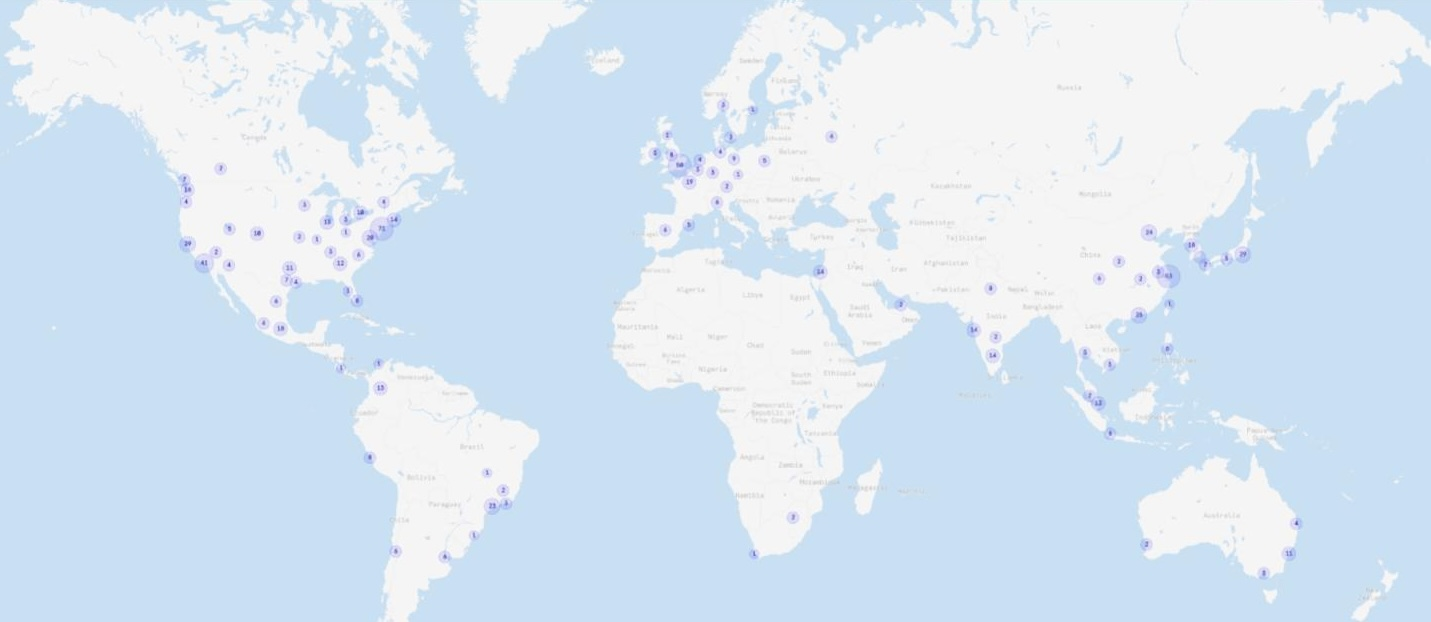
\includegraphics{assets/WeWork/WeWorkMap.jpg}

}

\caption{Global Footprint}

\end{figure}%

\subsubsection{Entreprise Projects}\label{entreprise-projects}

\paragraph{Parnassus Tower Amsterdam}\label{parnassus-tower-amsterdam}

\begin{figure}[H]

{\centering 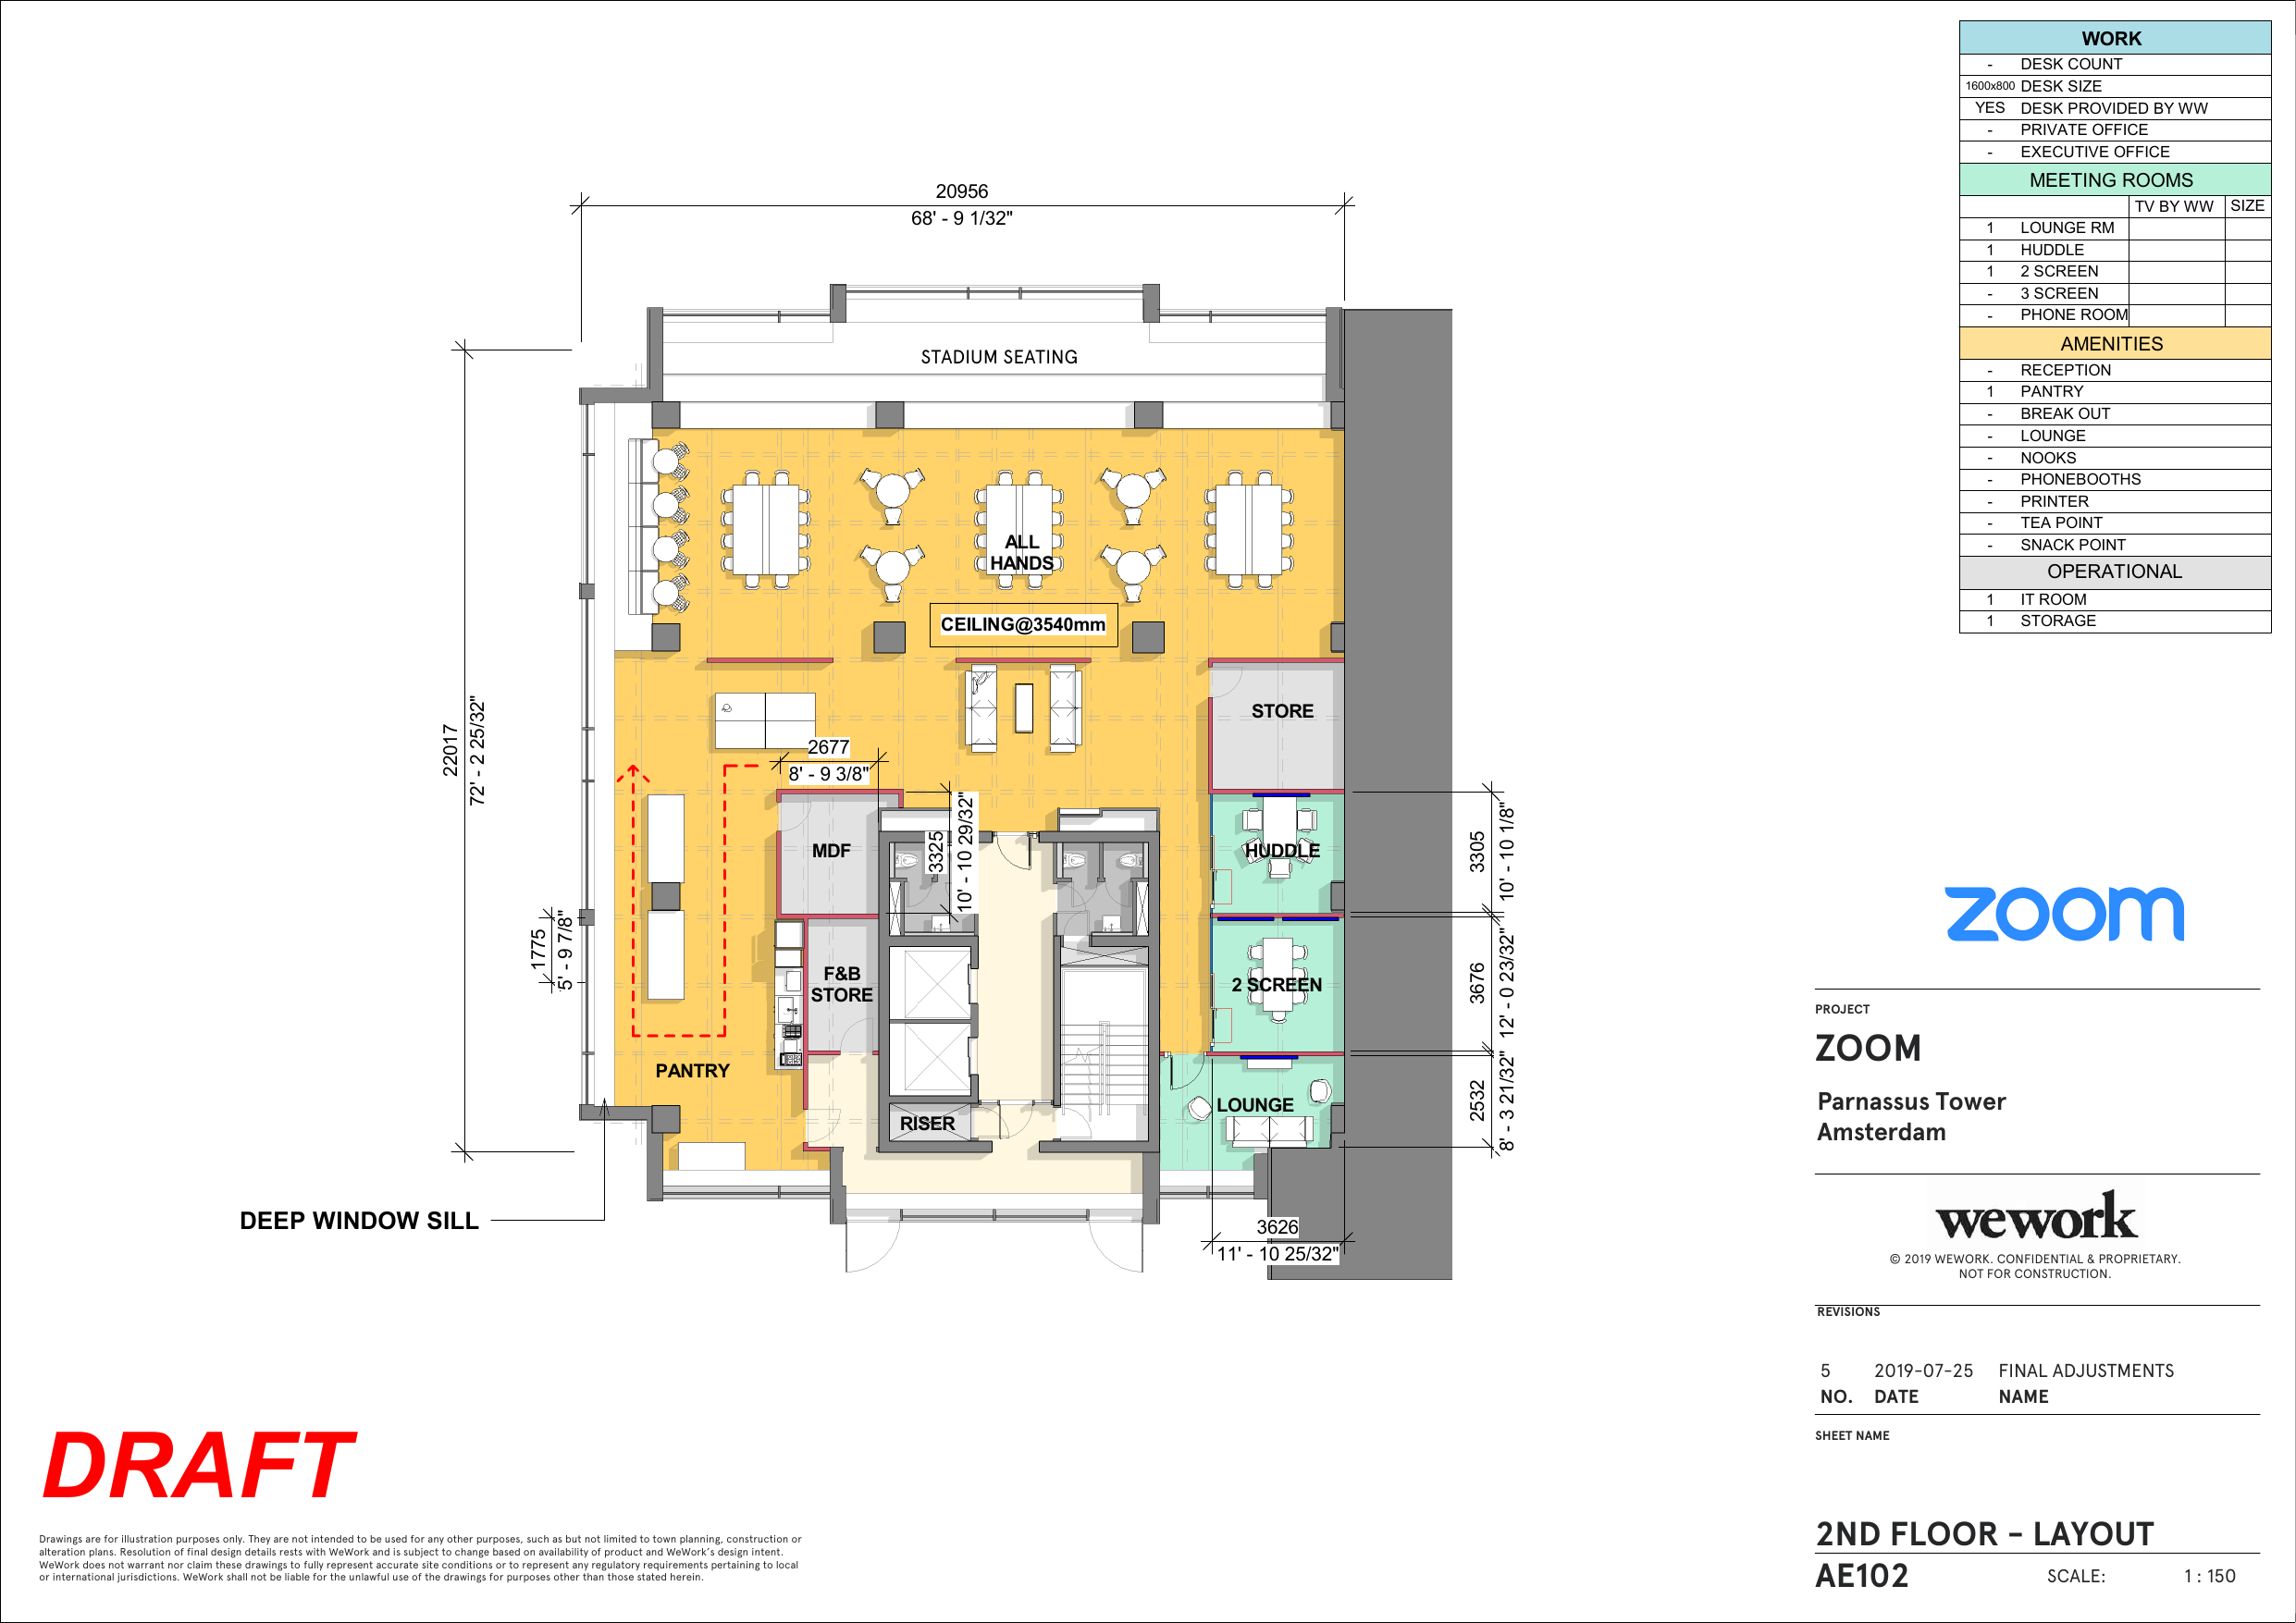
\includegraphics{assets/WeWork/ww-parnassus-2.png}

}

\caption{WeWork\_1}

\end{figure}%%
\begin{figure}[H]

{\centering 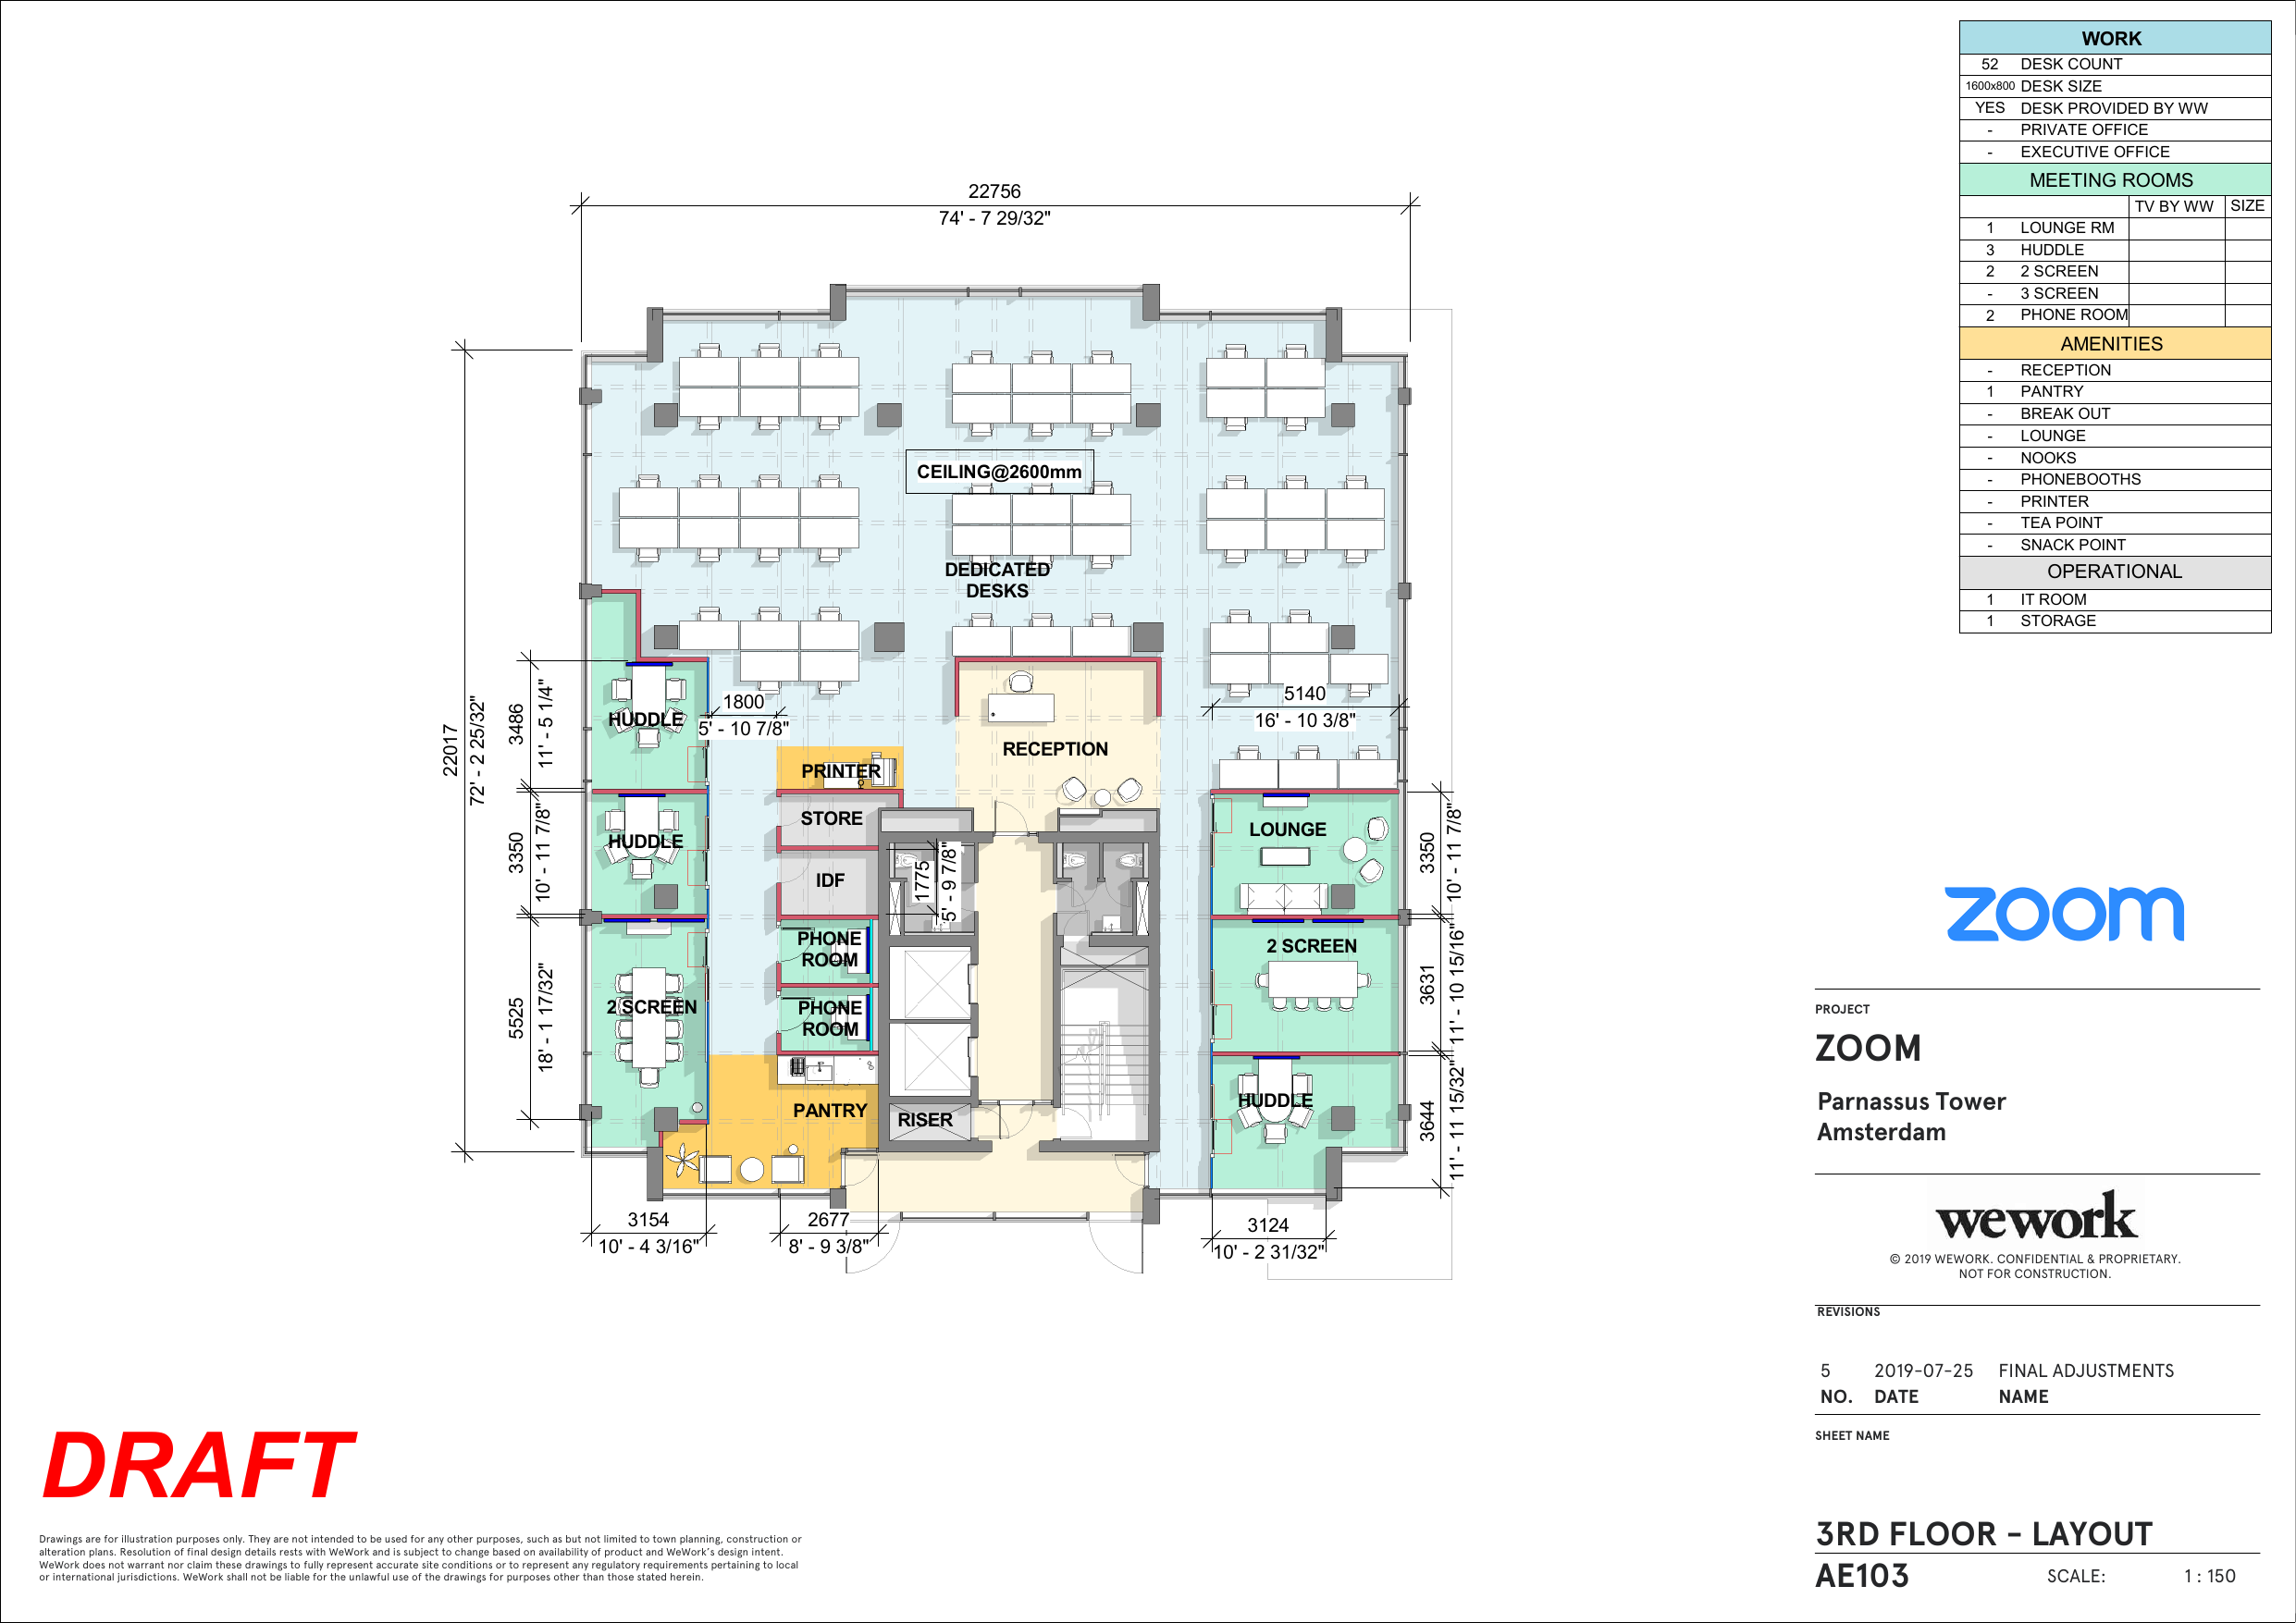
\includegraphics{assets/WeWork/ww-parnassus-3.png}

}

\caption{WeWork\_2}

\end{figure}%%
\begin{figure}[H]

{\centering 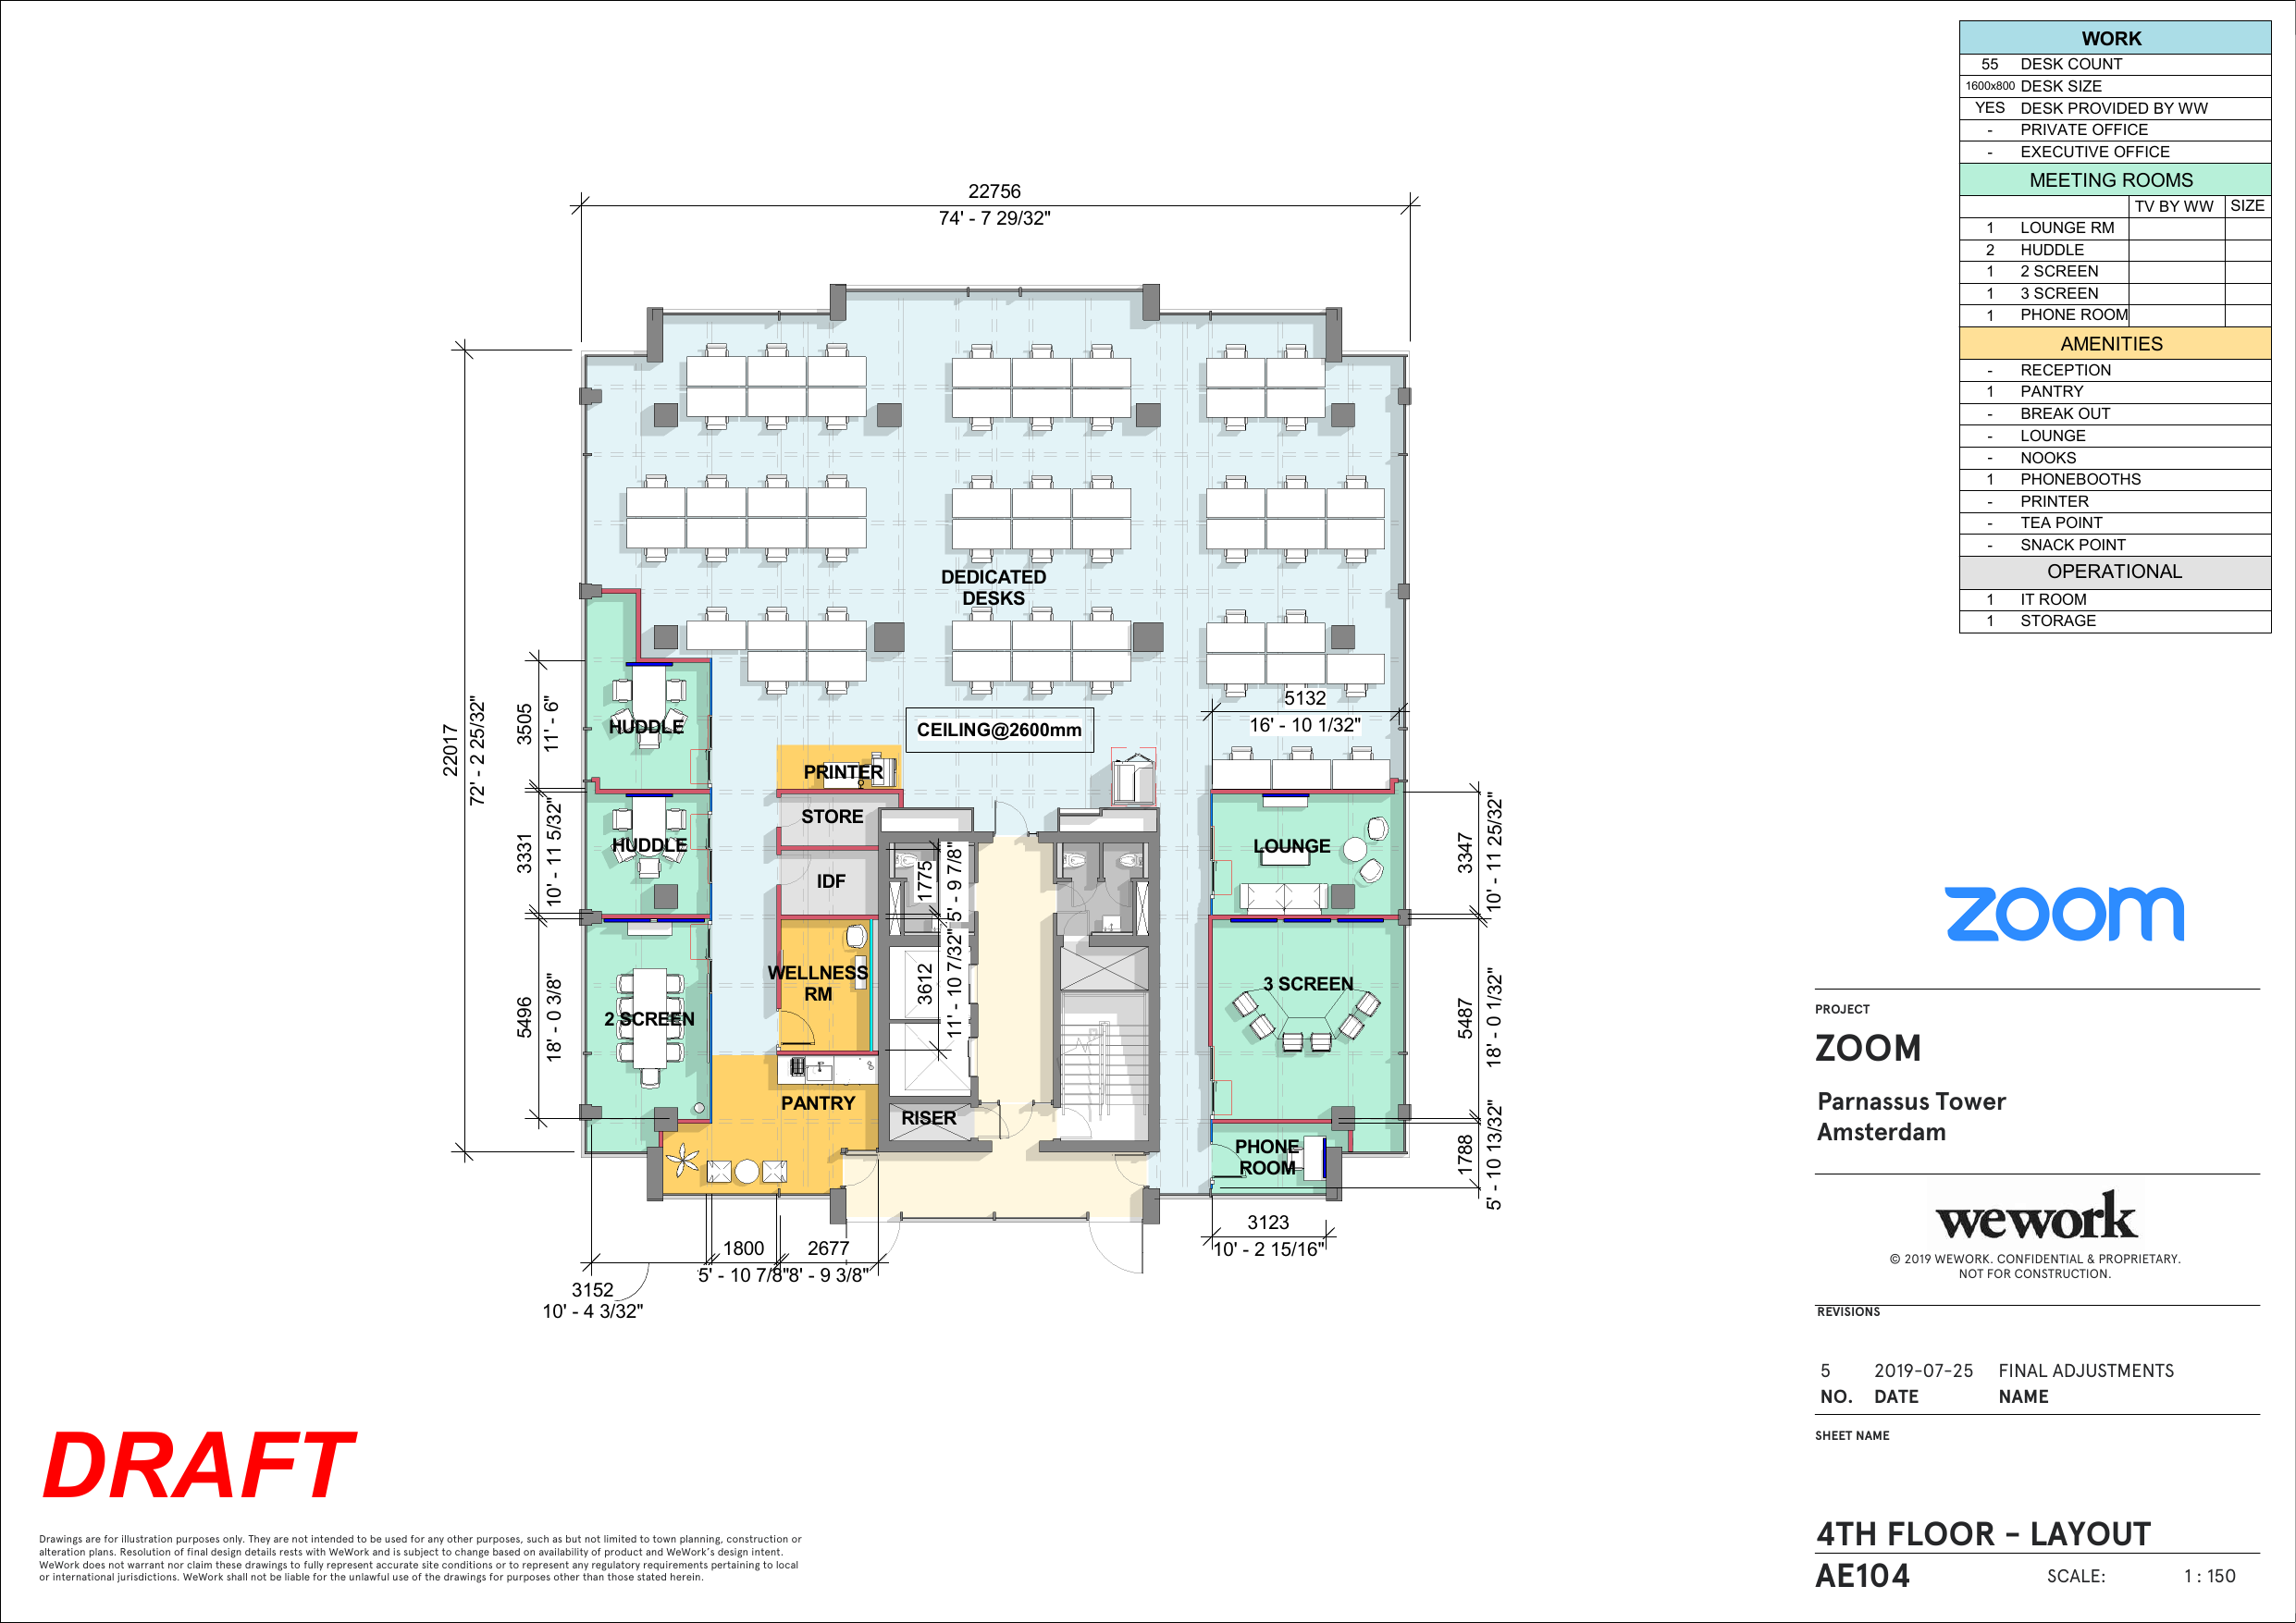
\includegraphics{assets/WeWork/ww-parnassus-4.png}

}

\caption{WeWork\_3}

\end{figure}%

\paragraph{Amazon Hannover Building,
Manchester}\label{amazon-hannover-building-manchester}

\begin{figure}[H]

{\centering 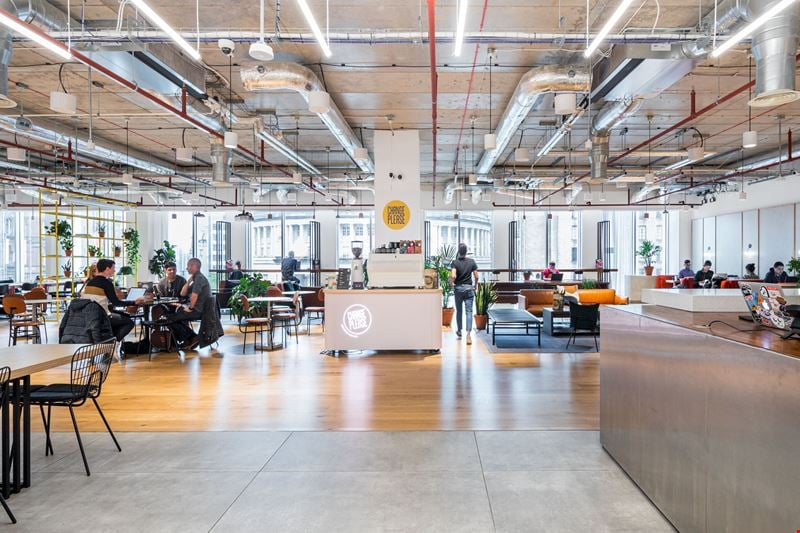
\includegraphics{assets/WeWork/WW_hannover.jpg}

}

\caption{WeWork\_hannover}

\end{figure}%

\subsubsection{BIM at WeWork}\label{bim-at-wework}

\begin{quote}
WeWork uses Autodesk building information modeling (BIM) software
throughout the building lifecycle to help keep pace with the growing
demand for collaborative office space around the world.
\end{quote}

\paragraph{Reality Capture - BIM for existing
conditions}\label{reality-capture---bim-for-existing-conditions}

Capturing accurate as-built data as the first step of design

\begin{quote}
WeWork uses reality capture and BIM solutions to support the design and
construction of its WeWork offices, including ReCap, Revit, and Dynamo
software. The firm uses 3D laser scanners to capture the existing
conditions of a newly acquired space. The resulting point clouds are
combined and edited in ReCap to visualize and navigate the existing
conditions data. This data is used in Revit to guide WeWork's modeling
efforts as it develops a series of design options. The firm uses Dynamo
and Revit API to embed cost and sales data from its business systems in
the models in order to analyze revenue versus cost and other key
business metrics.
\end{quote}

\begin{figure}[H]

{\centering 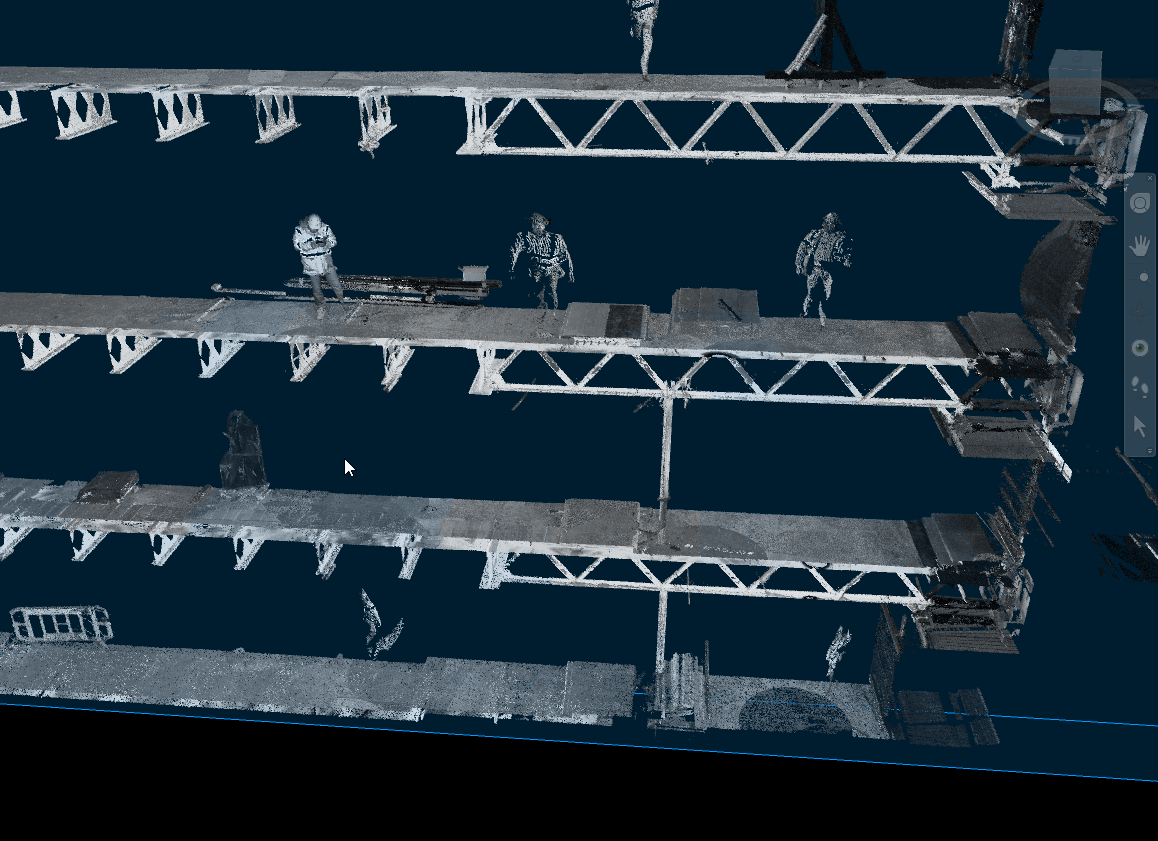
\includegraphics{assets/WeWork/WeWork-PointCloud-Coordination4.png}

}

\caption{WeWork\_}

\end{figure}%%
\begin{figure}[H]

{\centering 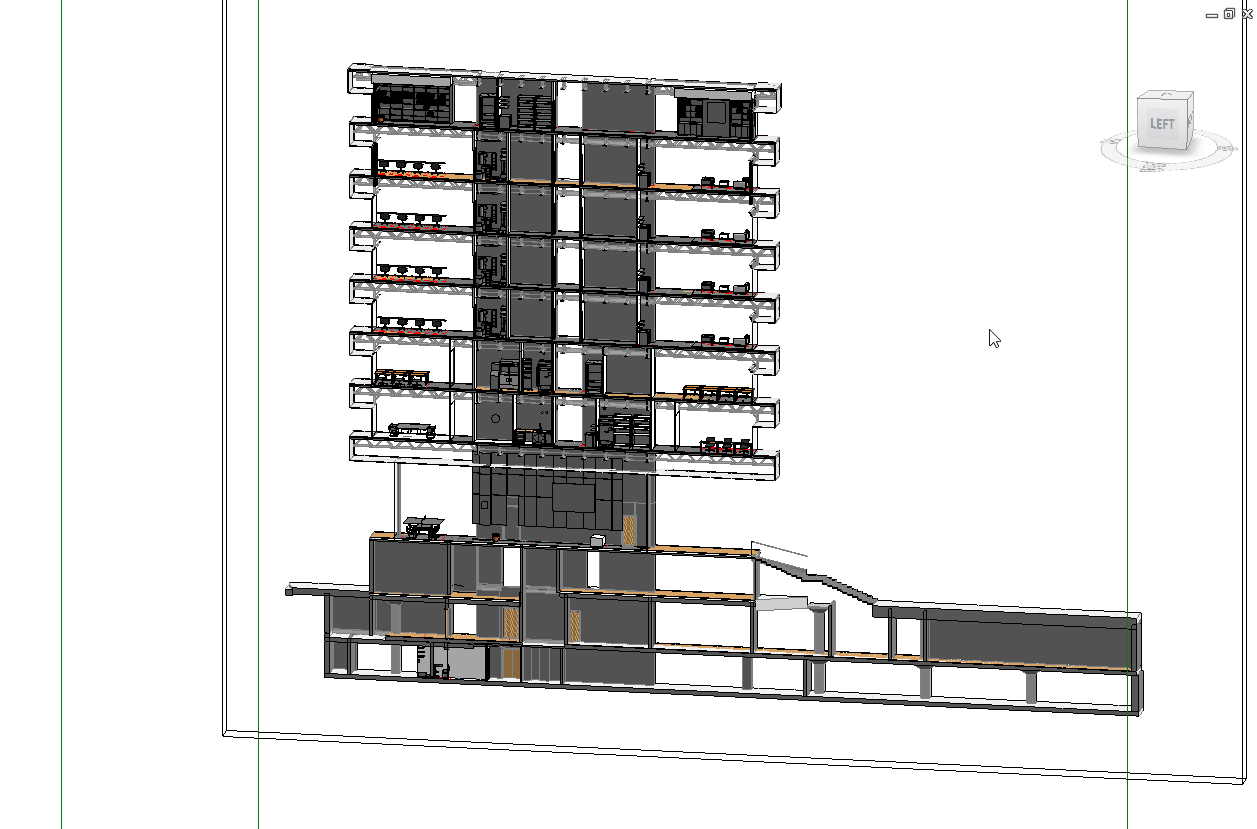
\includegraphics{assets/WeWork/WeWork-Point-Cloud-Coordination-36-Dame.png}

}

\caption{WeWork\_}

\end{figure}%%
\begin{figure}[H]

{\centering 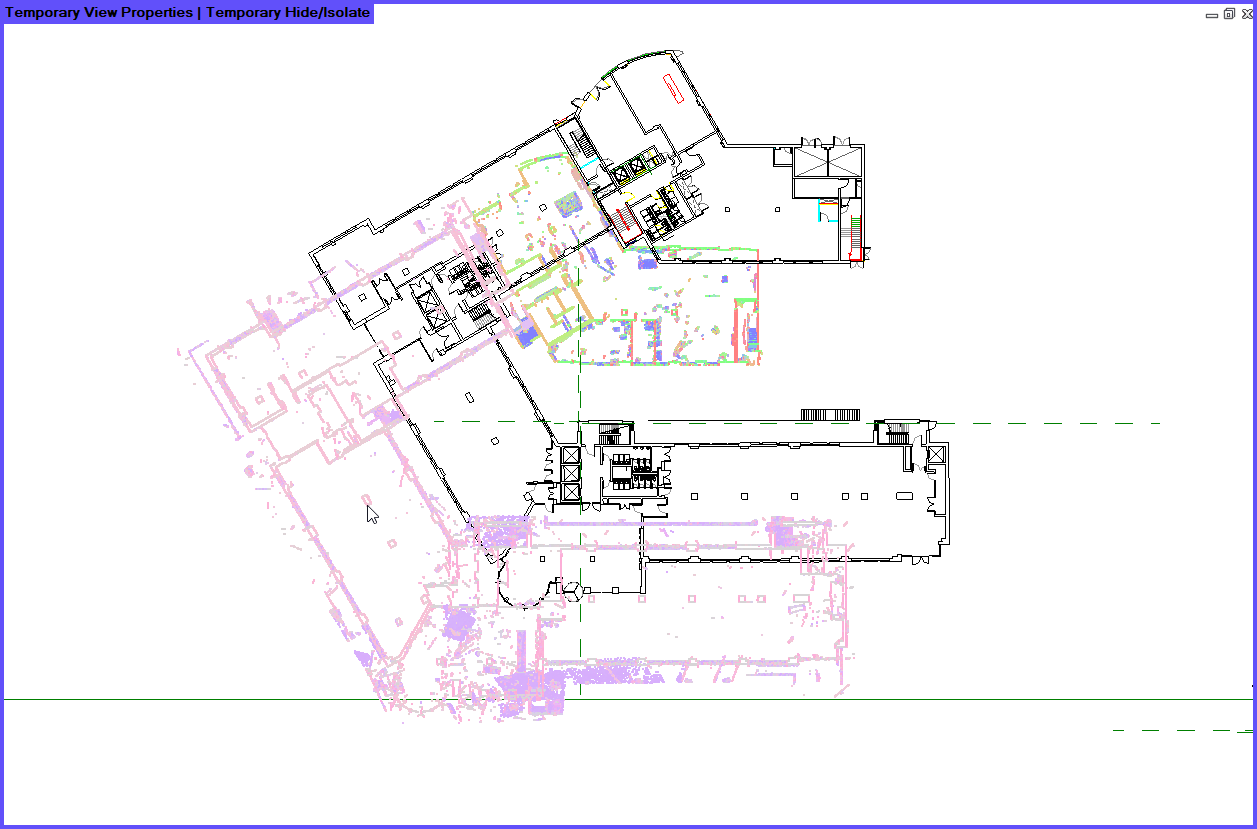
\includegraphics{assets/WeWork/WeWork-PointCloud-Coordination-2.png}

}

\caption{WeWork\_}

\end{figure}%%
\begin{figure}[H]

{\centering 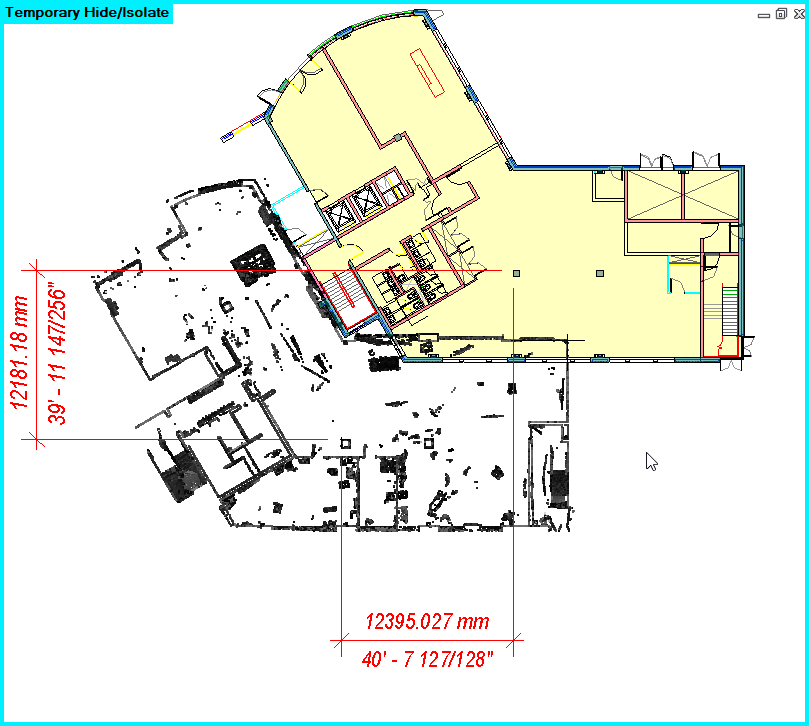
\includegraphics{assets/WeWork/WeWork-PointCloud-Coordination.png}

}

\caption{WeWork\_}

\end{figure}%

\paragraph{Tooled up BIM, PyRevit, Dynamo, Google Apps
Scripts}\label{tooled-up-bim-pyrevit-dynamo-google-apps-scripts}

\begin{quote}
As the design progresses, WeWork scans the space and references that
data to quickly generate a more detailed design model and coordinate its
design with existing structure and services. This highly-coordinated,
precise 3D model offers increased use of prefabrication and offsite
assembly, helping to minimize onsite rework and avoid delays during
construction. In addition, the intelligent Revit design model drives
WeWork's supply chain. With Revit, the project team is able to produce
all of their drawings and quantities automatically, so all estimating
and bidding is based on the design model and surprises are minimized
during construction.
\end{quote}

\begin{figure}[H]

{\centering 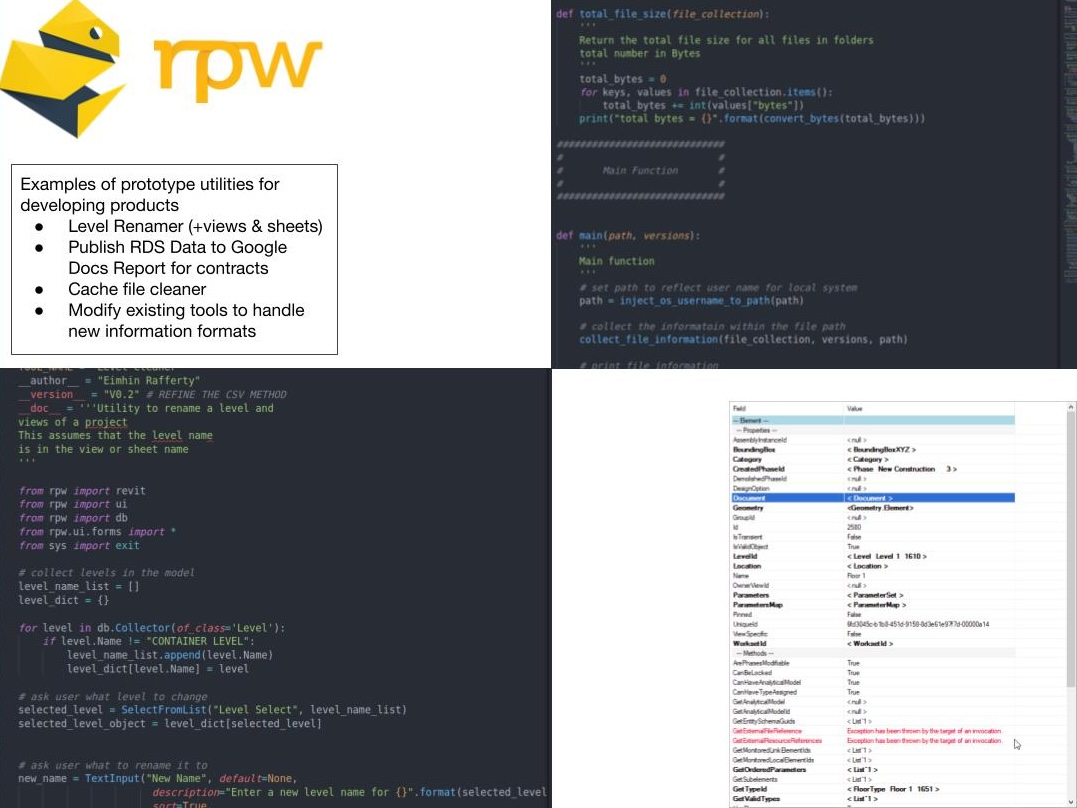
\includegraphics{assets/WeWork/WeWorkTools.jpg}

}

\caption{WeWork\_Pytools}

\end{figure}%%
\begin{figure}[H]

{\centering 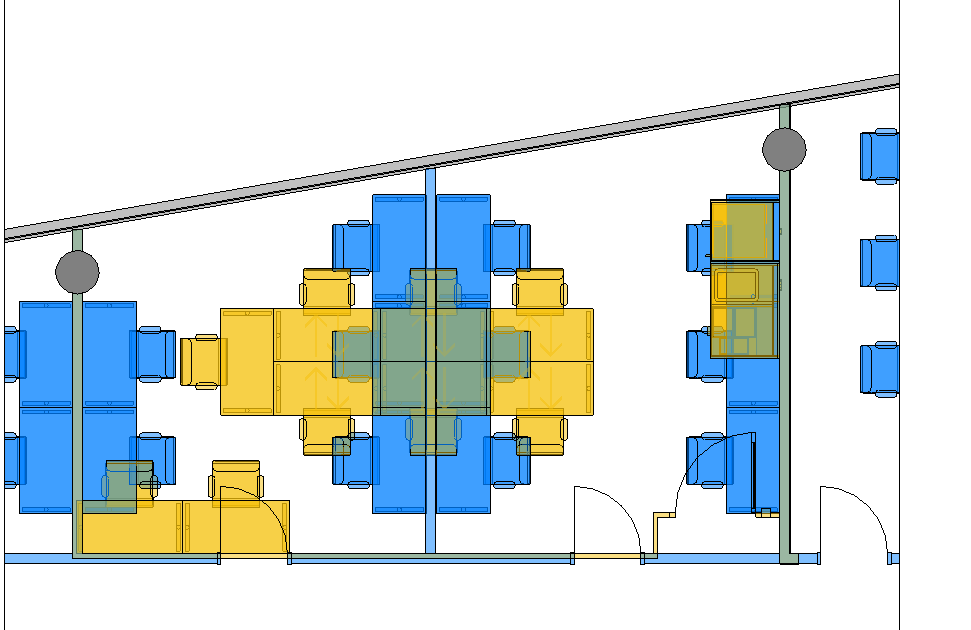
\includegraphics{assets/WeWork/WeWork-Coodinatoin-As-Built.png}

}

\caption{WeWork\_}

\end{figure}%%
\begin{figure}[H]

{\centering \includegraphics{assets/WeWork/WeWork-Automation-Gsheet-MAAnnex.gif}

}

\caption{WeWork\_}

\end{figure}%%
\begin{figure}[H]

{\centering 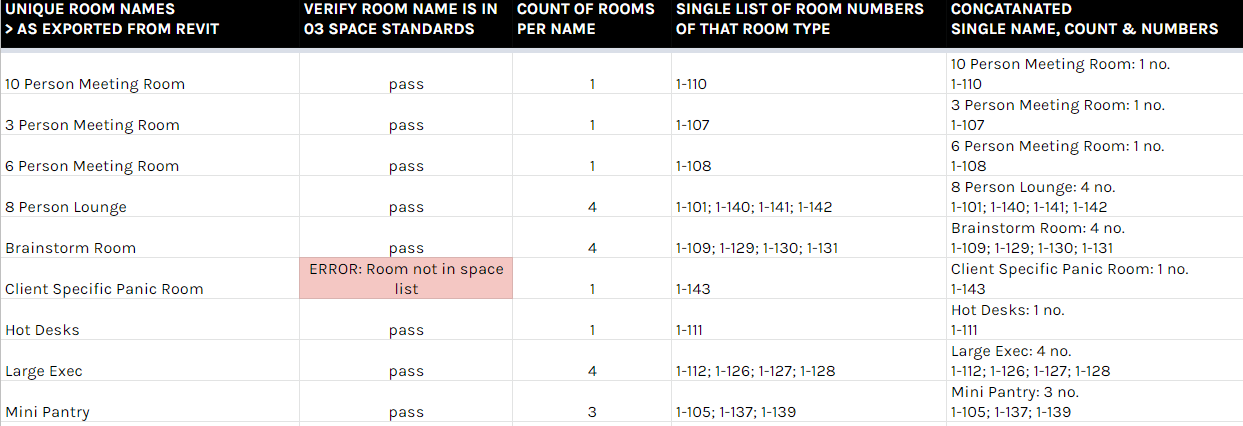
\includegraphics{assets/WeWork/WeWork-Automation-Gsheet-DataCheck.png}

}

\caption{WeWork\_}

\end{figure}%%
\begin{figure}[H]

{\centering 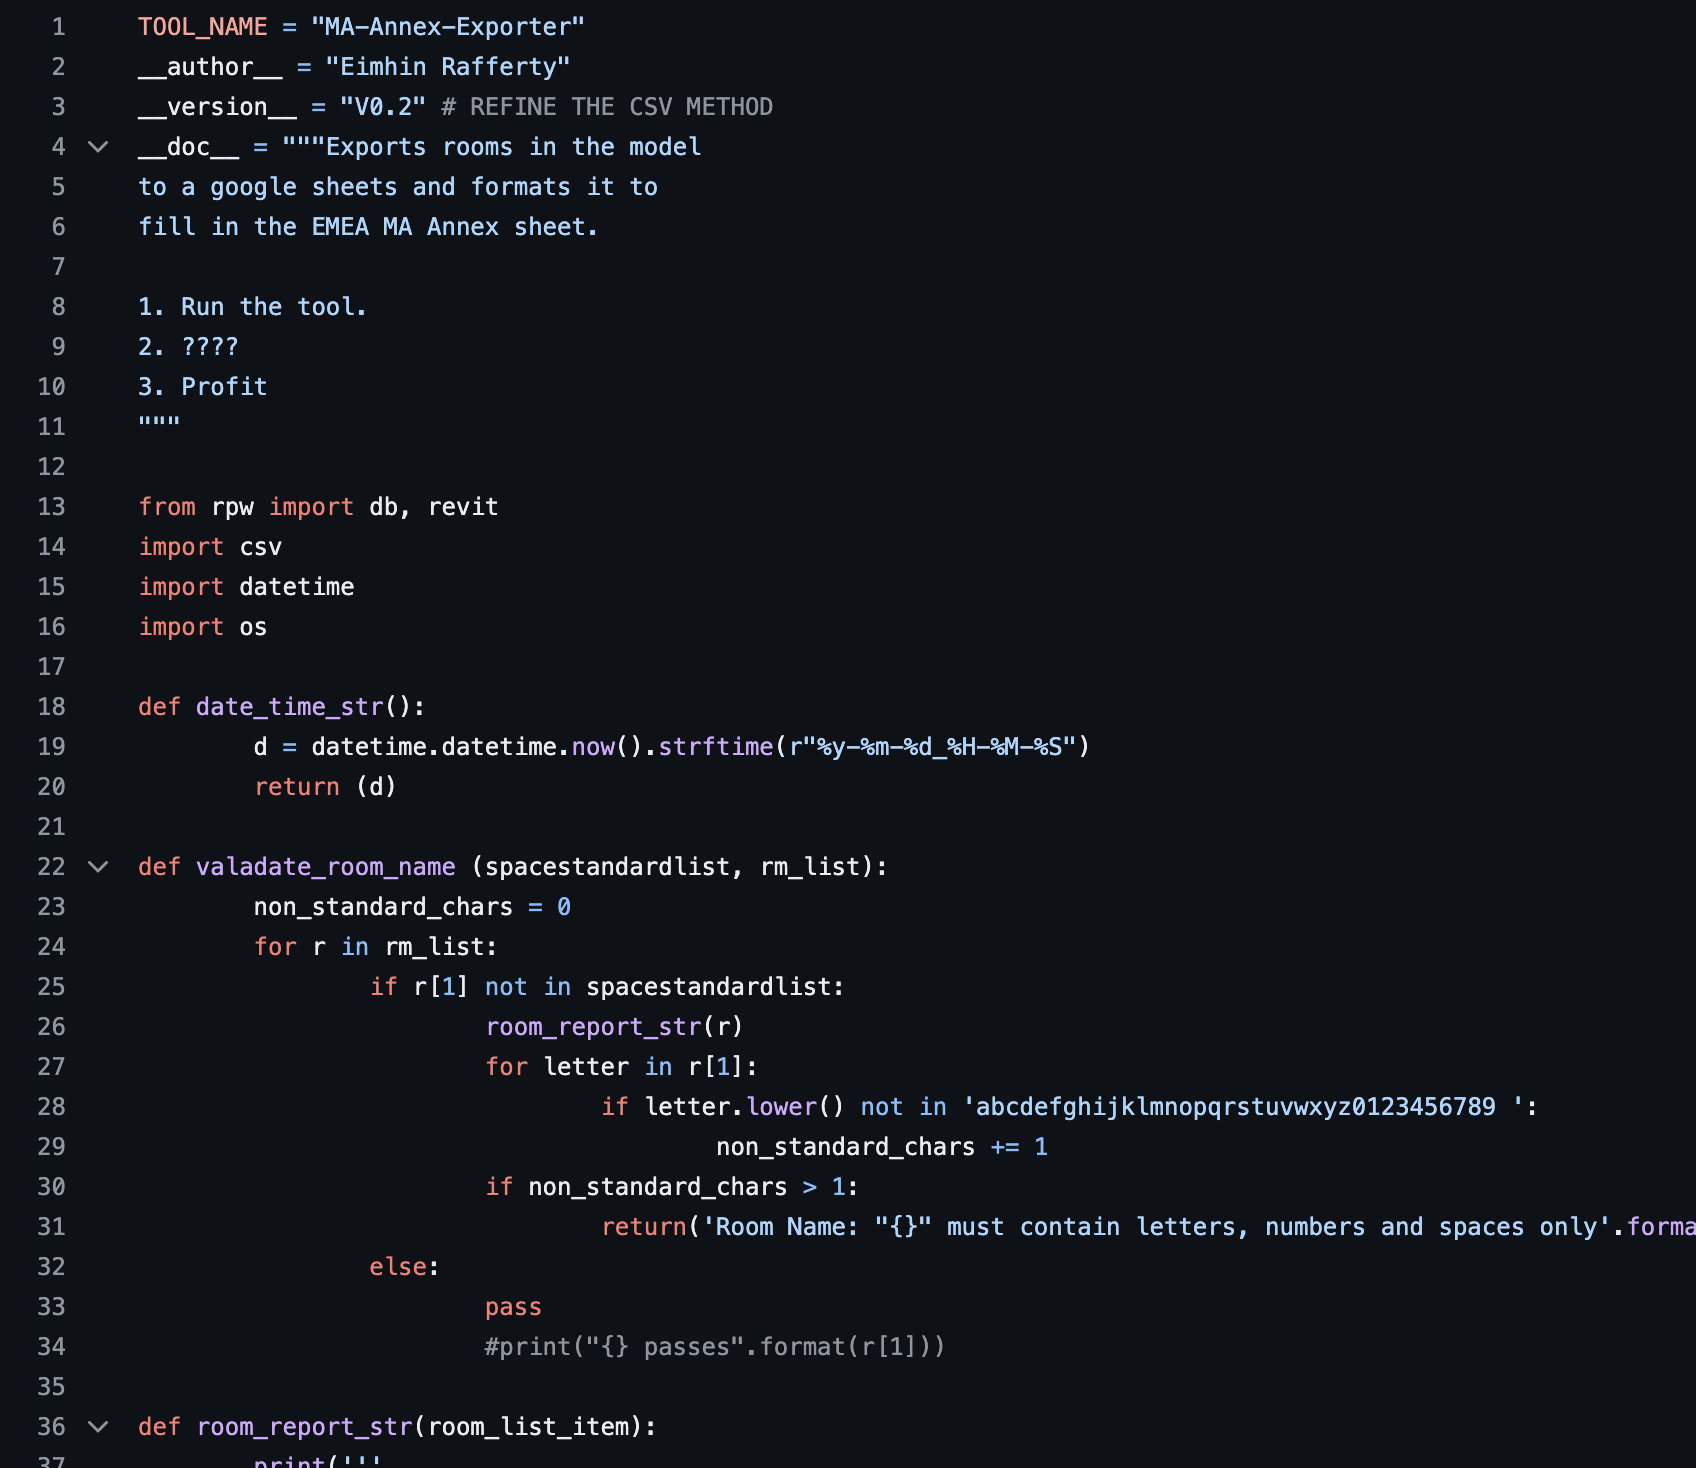
\includegraphics{assets/WeWork/CODEEXAMPLE1.png}

}

\caption{WW\_codeExamples}

\end{figure}%%
\begin{figure}[H]

{\centering 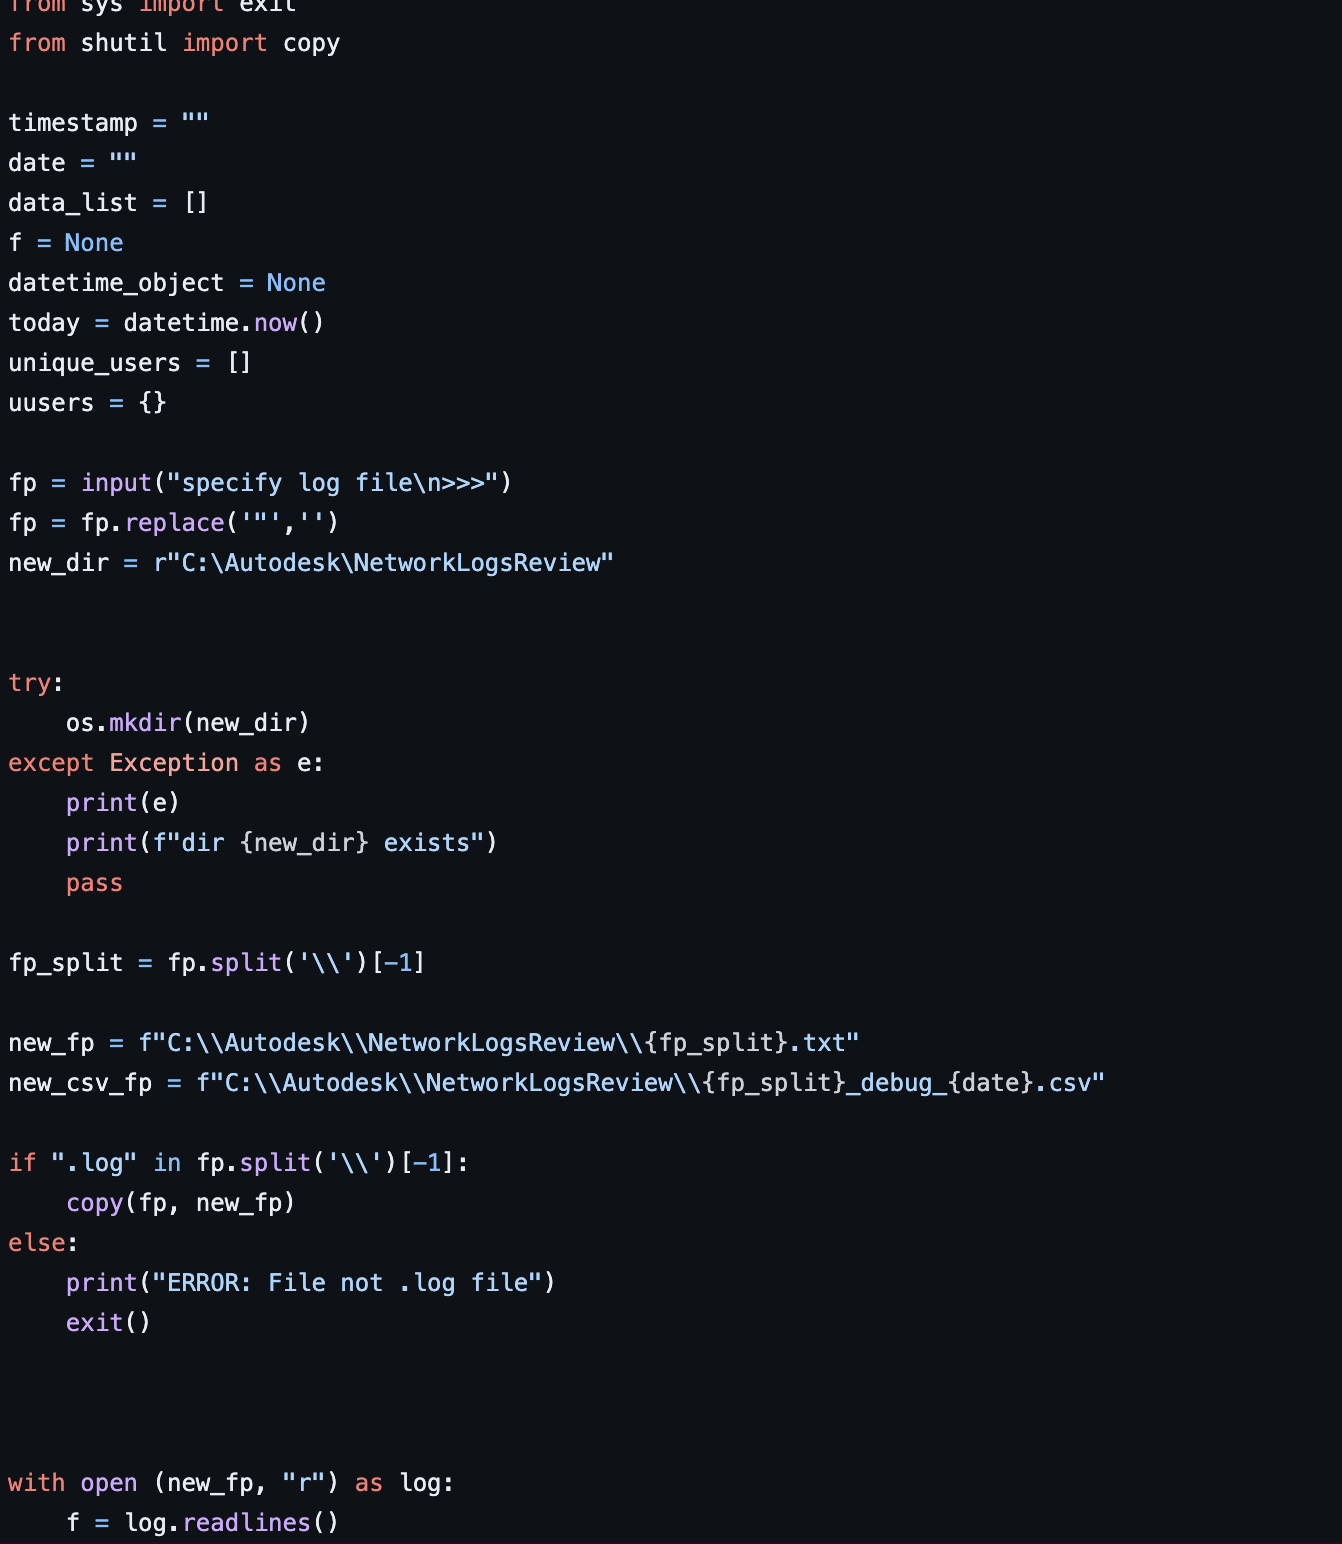
\includegraphics{assets/WeWork/CODEEXAMPLE2.png}

}

\caption{WW\_codeExamples}

\end{figure}%

\begin{Shaded}
\begin{Highlighting}[]
\CommentTok{/* Examples of simple SQL which enabled us to dive into our building data and}
\CommentTok{answer questions such as \textquotesingle{}hey how many MOP rooms are there in Florida?\textquotesingle{}  */}

\KeywordTok{select} 
\NormalTok{    s.UUID,}
\NormalTok{    s.floor\_uuid,}
\NormalTok{    s.ROOM\_NUMBER,}
\NormalTok{    s.DESIGNED\_AS\_SPACE\_TYPE,}
\NormalTok{    s.SQUARE\_FOOTAGE,}
\NormalTok{    s.WORK\_UNITS,}
\NormalTok{    s.DESK\_COUNT,}
\NormalTok{    s.HAS\_WINDOW,}
\NormalTok{    s.RGS\_SPACE\_TYPE,}
\NormalTok{    f.}\KeywordTok{LABEL}\NormalTok{,}
\NormalTok{    f.UUID,}
\NormalTok{    f.BUILDING\_UUID,}
\NormalTok{    f.SPACE\_FIRST\_PHYSICAL\_OPEN\_DATE,}
\NormalTok{    b.COUNTRY,}
\NormalTok{    b.STATE,}
\NormalTok{    b.CITY,}
\NormalTok{    b.ADDRESS\_LINE,}
\NormalTok{    b.NAME,}
\NormalTok{    b.UUID}
\KeywordTok{FROM}\NormalTok{ CENTRAL.CDM\_PHYSICAL\_SPACE.SPACE }\KeywordTok{AS}\NormalTok{ s}
  \KeywordTok{INNER} \KeywordTok{JOIN}\NormalTok{ CENTRAL.CDM\_PHYSICAL\_SPACE.}\FunctionTok{FLOOR} \KeywordTok{AS}\NormalTok{ f }\KeywordTok{on}\NormalTok{ f.UUID }\OperatorTok{=}\NormalTok{ s.floor\_uuid}
  \KeywordTok{INNER} \KeywordTok{JOIN}\NormalTok{ CENTRAL.CDM\_PHYSICAL\_SPACE.BUILDING }\KeywordTok{AS}\NormalTok{ b }\KeywordTok{on}\NormalTok{ b.uuid }\OperatorTok{=}\NormalTok{ f.BUILDING\_UUID}
       \KeywordTok{WHERE}\NormalTok{ s.DESIGNED\_AS\_SPACE\_TYPE }\OperatorTok{=}\StringTok{\textquotesingle{}MOP\textquotesingle{}} 
         \KeywordTok{AND}\NormalTok{ s.SQUARE\_FOOTAGE }\KeywordTok{BETWEEN} \DecValTok{900} \KeywordTok{AND} \DecValTok{1100}
         \KeywordTok{AND}\NormalTok{ b.STATE }\KeywordTok{LIKE} \StringTok{\textquotesingle{}Florida\textquotesingle{}}
    \KeywordTok{ORDER} \KeywordTok{BY}\NormalTok{ s.SQUARE\_FOOTAGE }\KeywordTok{DESC}
\end{Highlighting}
\end{Shaded}

\paragraph{Design Standards Content + Process +
Traning}\label{design-standards-content-process-traning}

\begin{itemize}
\tightlist
\item
  Initiative to give teams the tools to implement design standards.
\item
  Self documenting content.
\item
  Reliable, maintainable, version controled documentation.
\item
  Formed the basis of consultant onboarding.
\end{itemize}

\begin{figure}[H]

{\centering \includegraphics{assets/WeWork/2019Q3-DesignContentUpdate_gimp.gif}

}

\caption{WeWork\_DesignContentGif}

\end{figure}%%
\begin{figure}[H]

{\centering 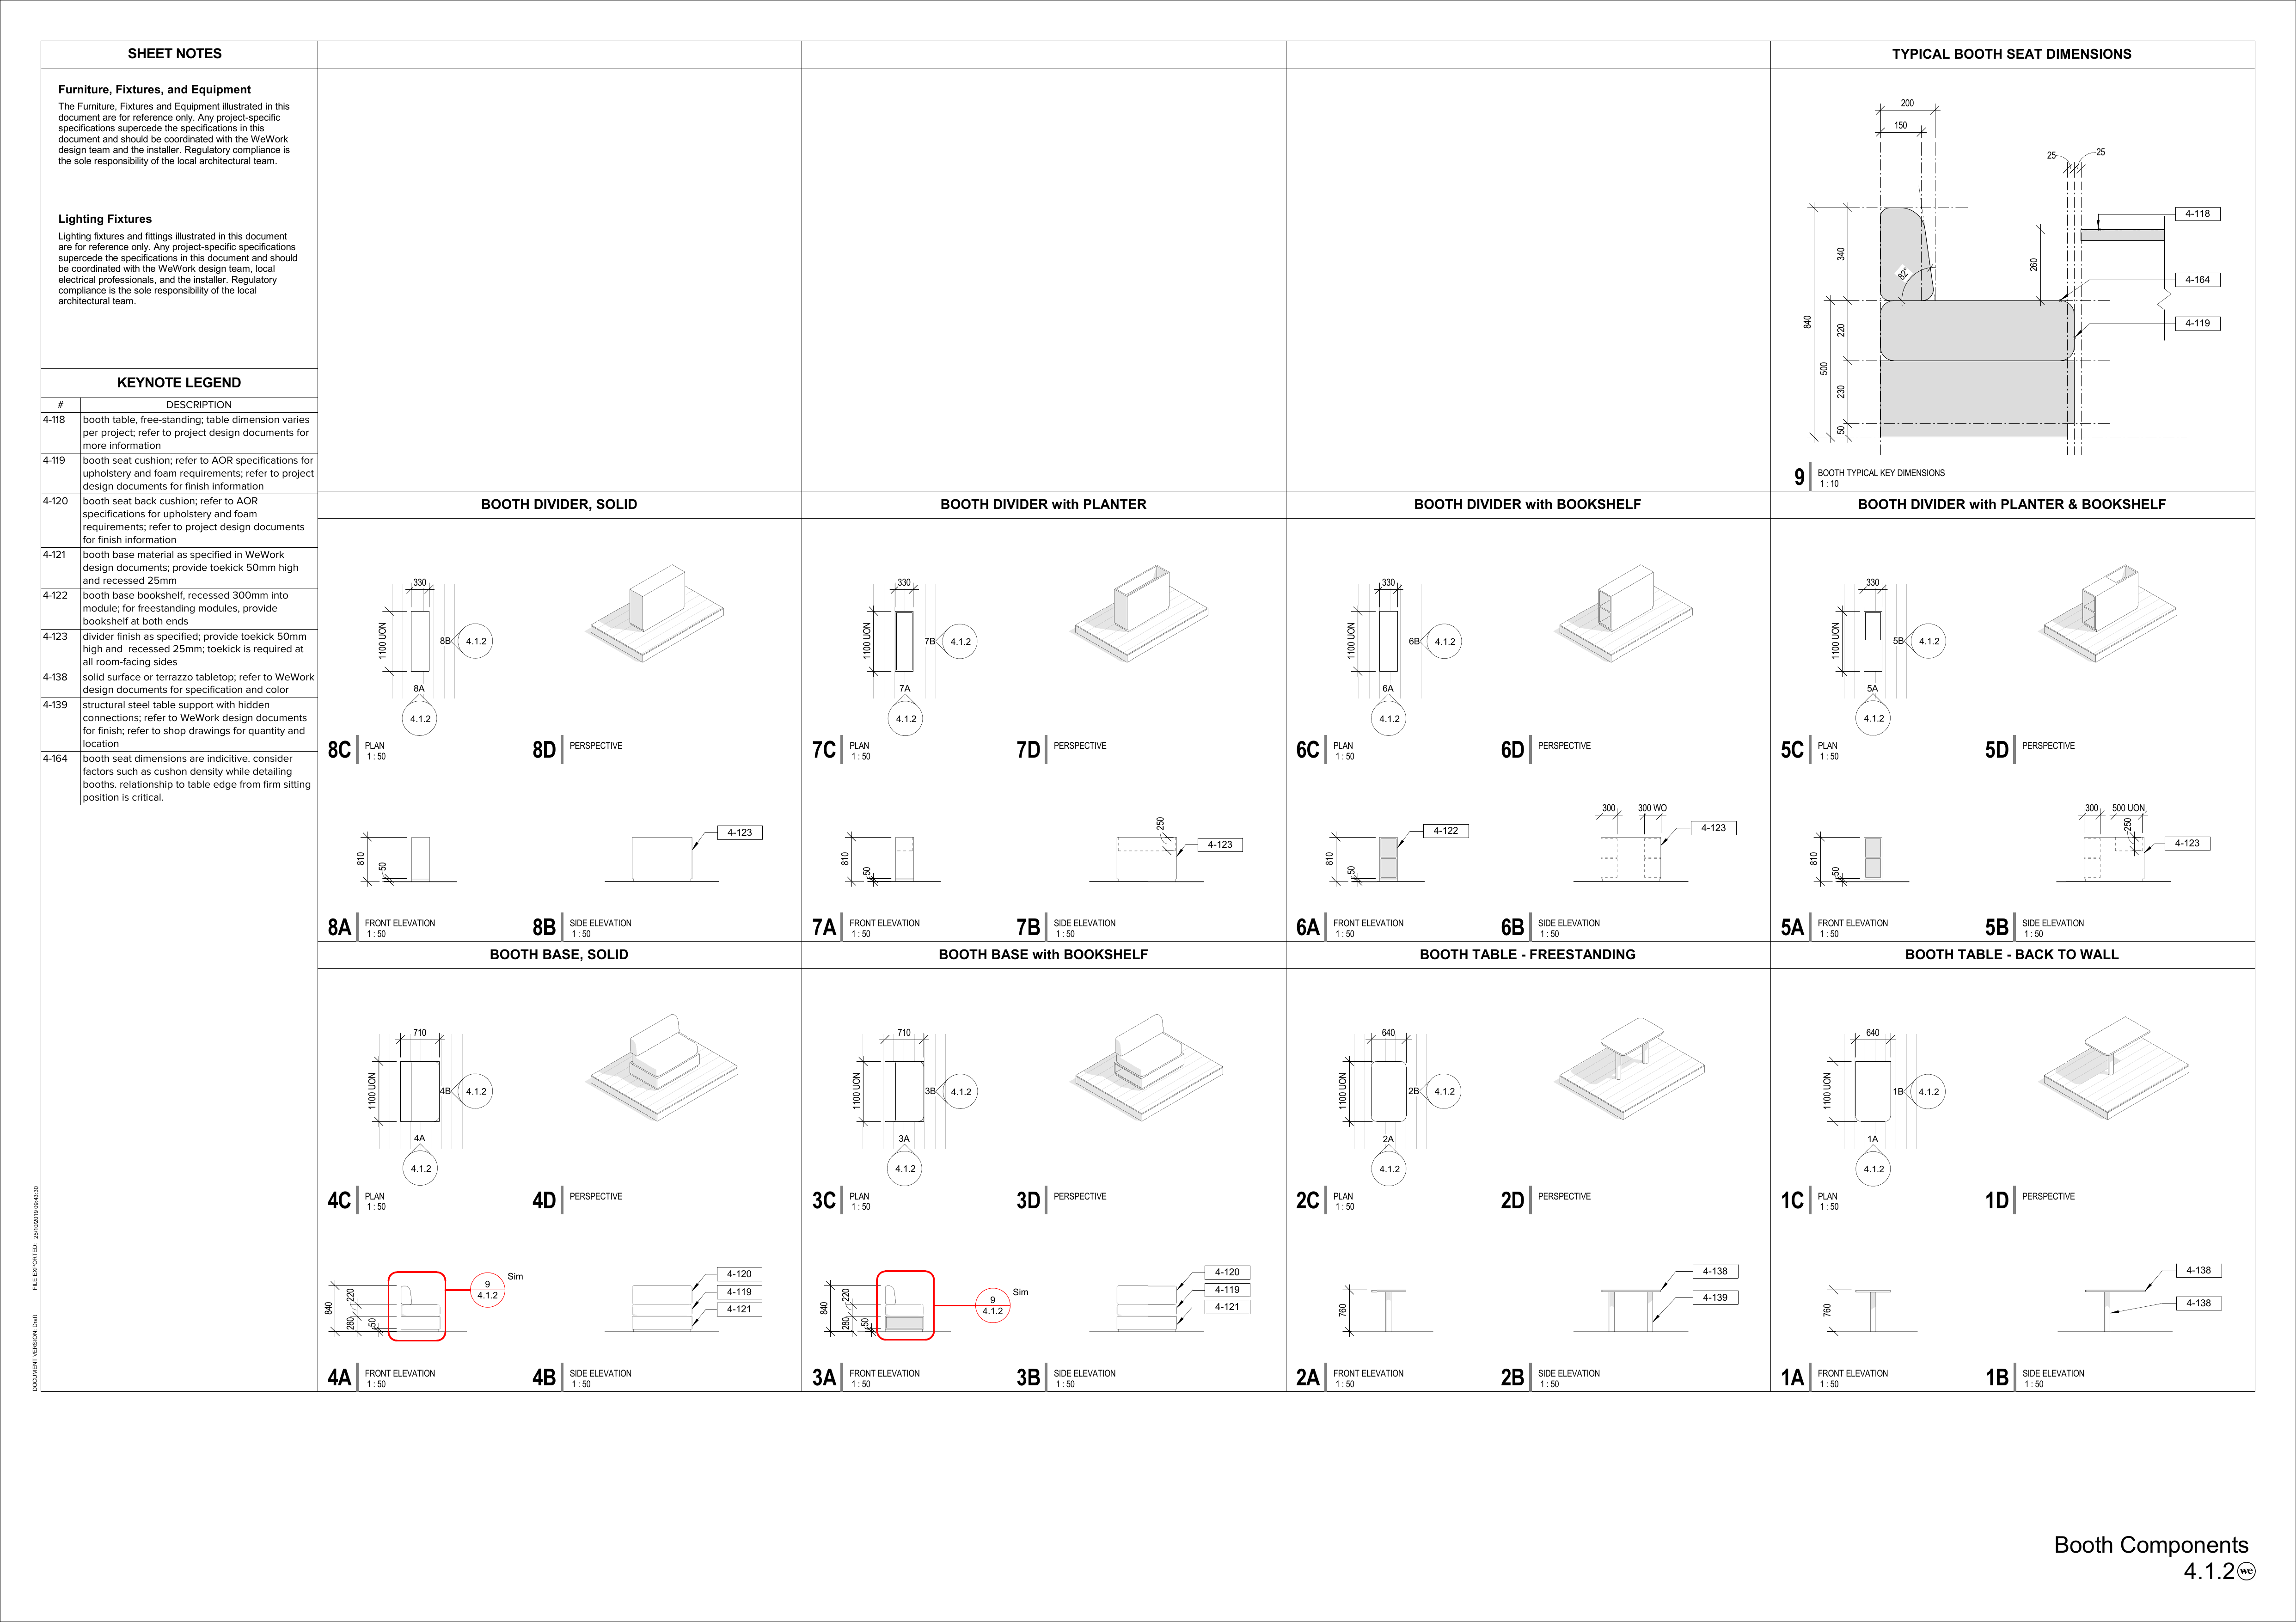
\includegraphics{assets/WeWork/ww_design_standards-16.png}

}

\caption{WeWork\_}

\end{figure}%%
\begin{figure}[H]

{\centering 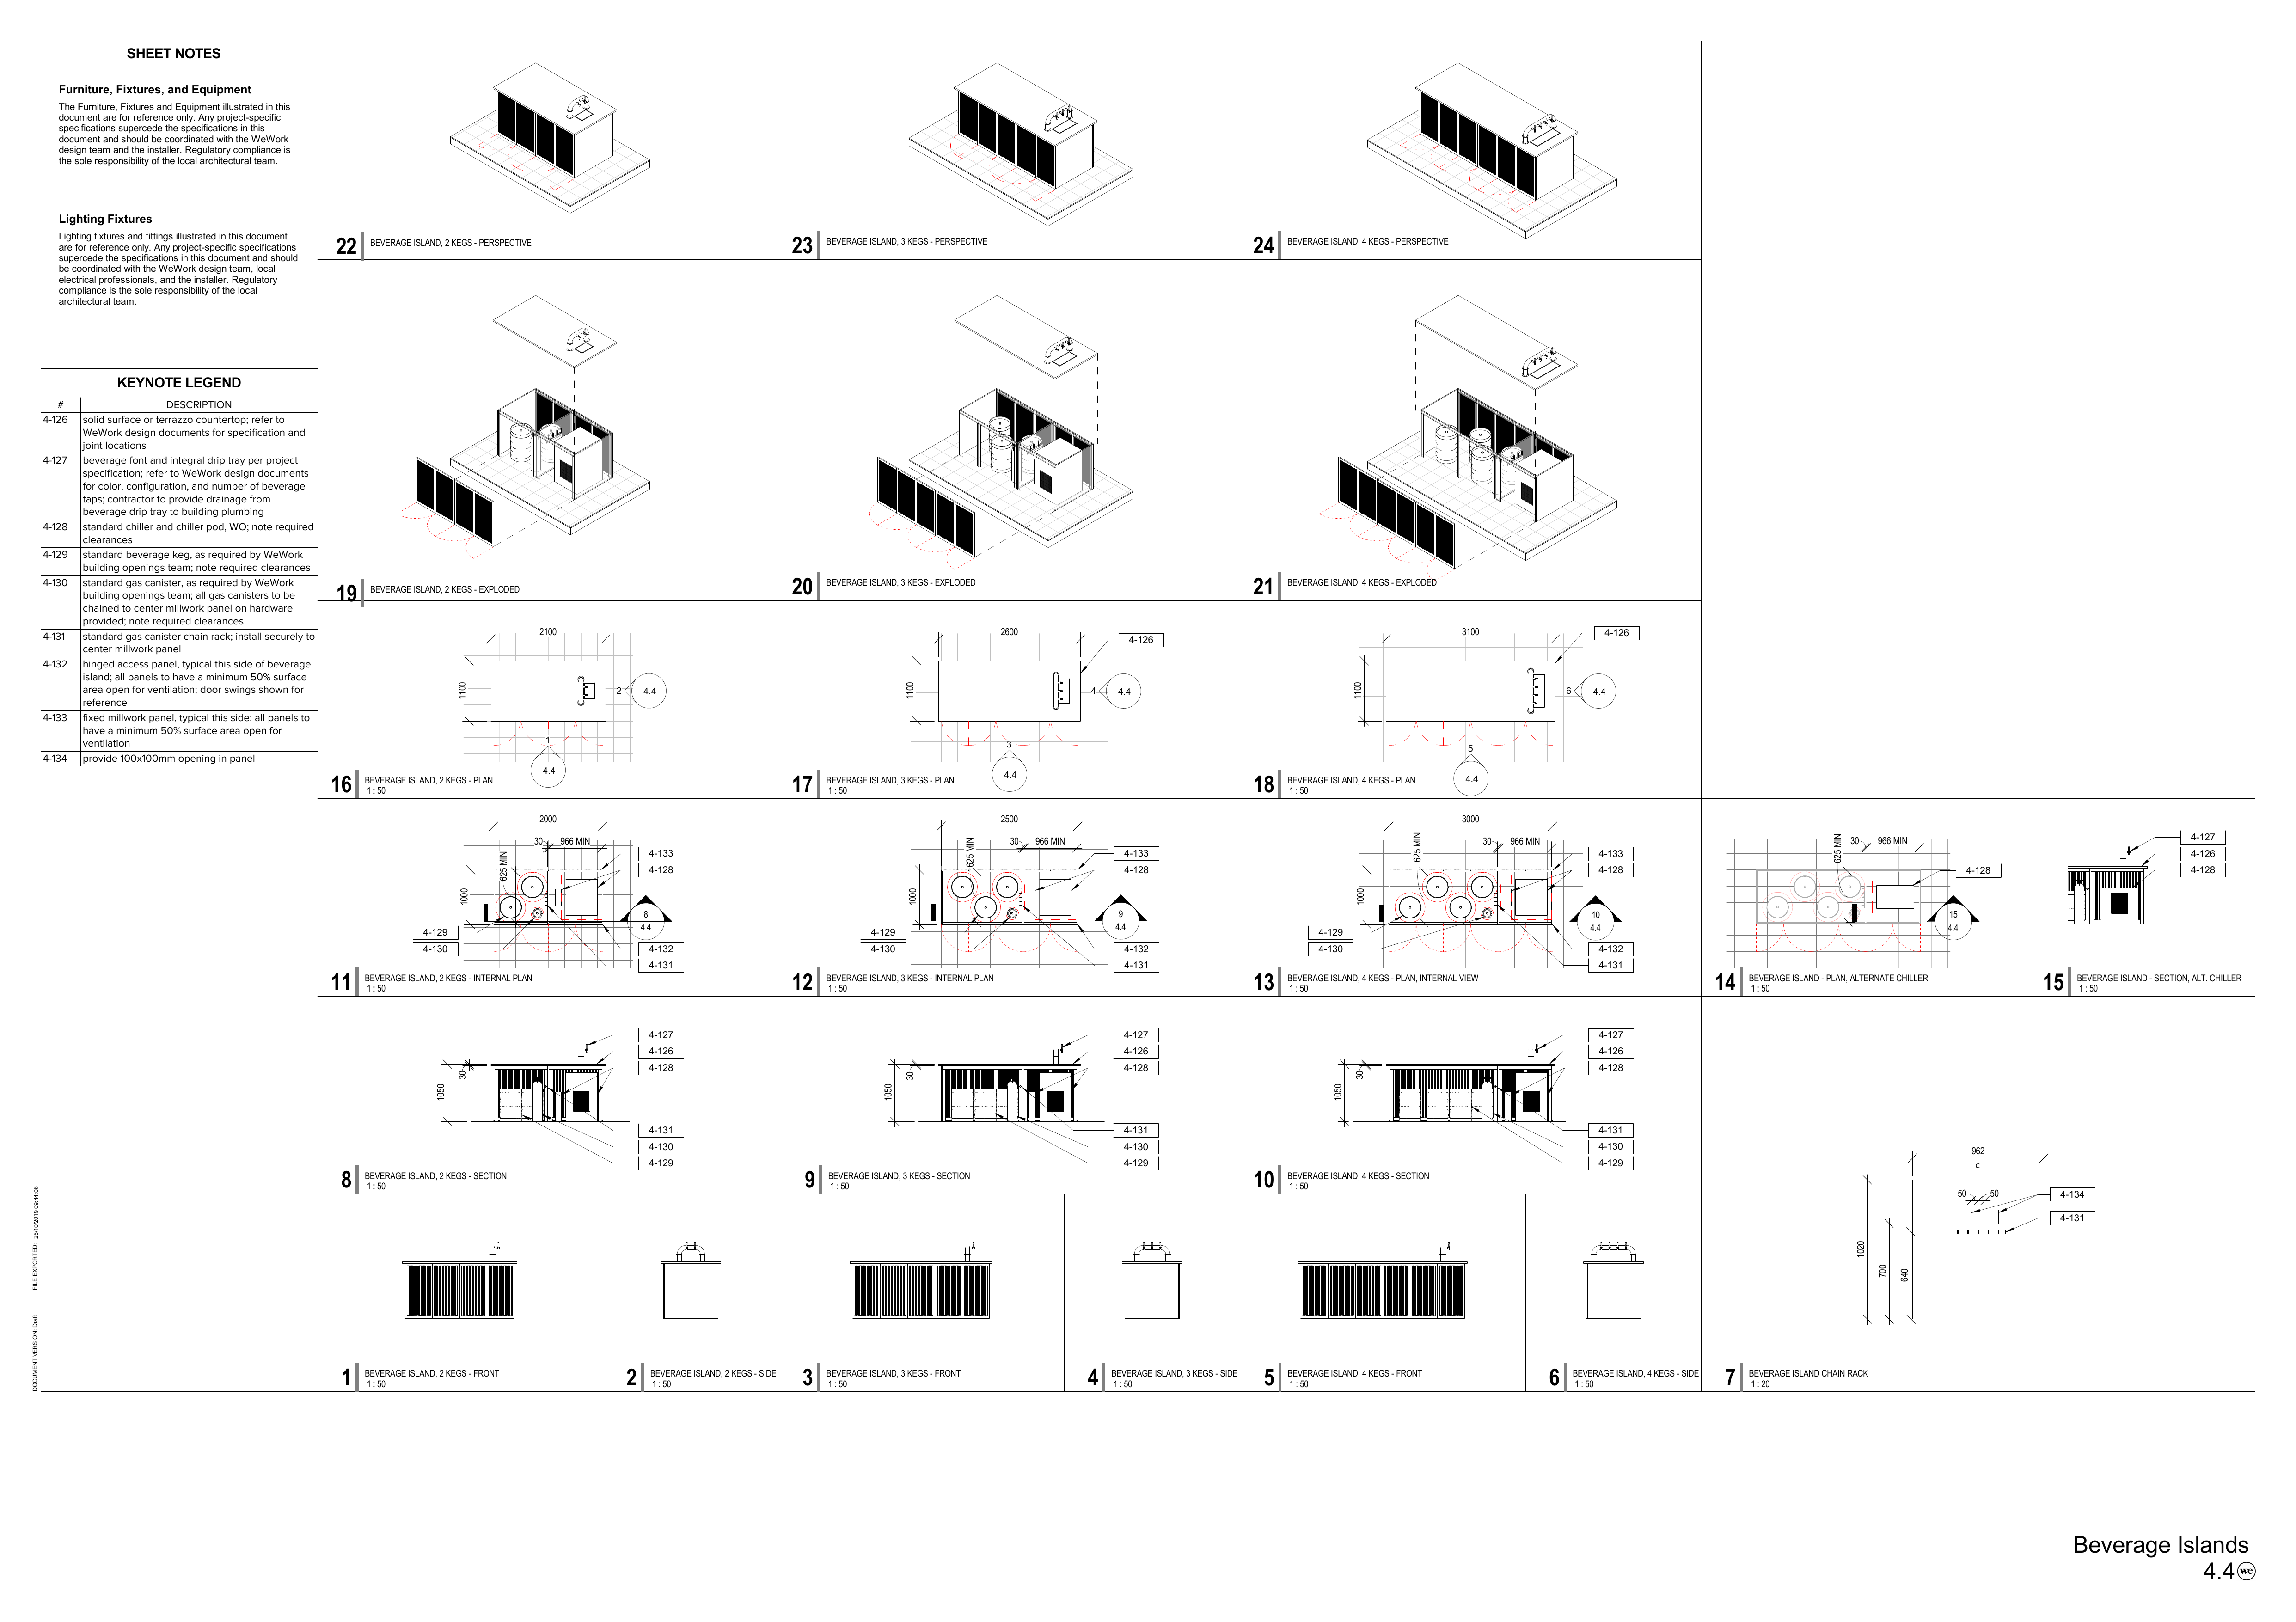
\includegraphics{assets/WeWork/ww_design_standards-19.png}

}

\caption{WeWork\_}

\end{figure}%%
\begin{figure}[H]

{\centering 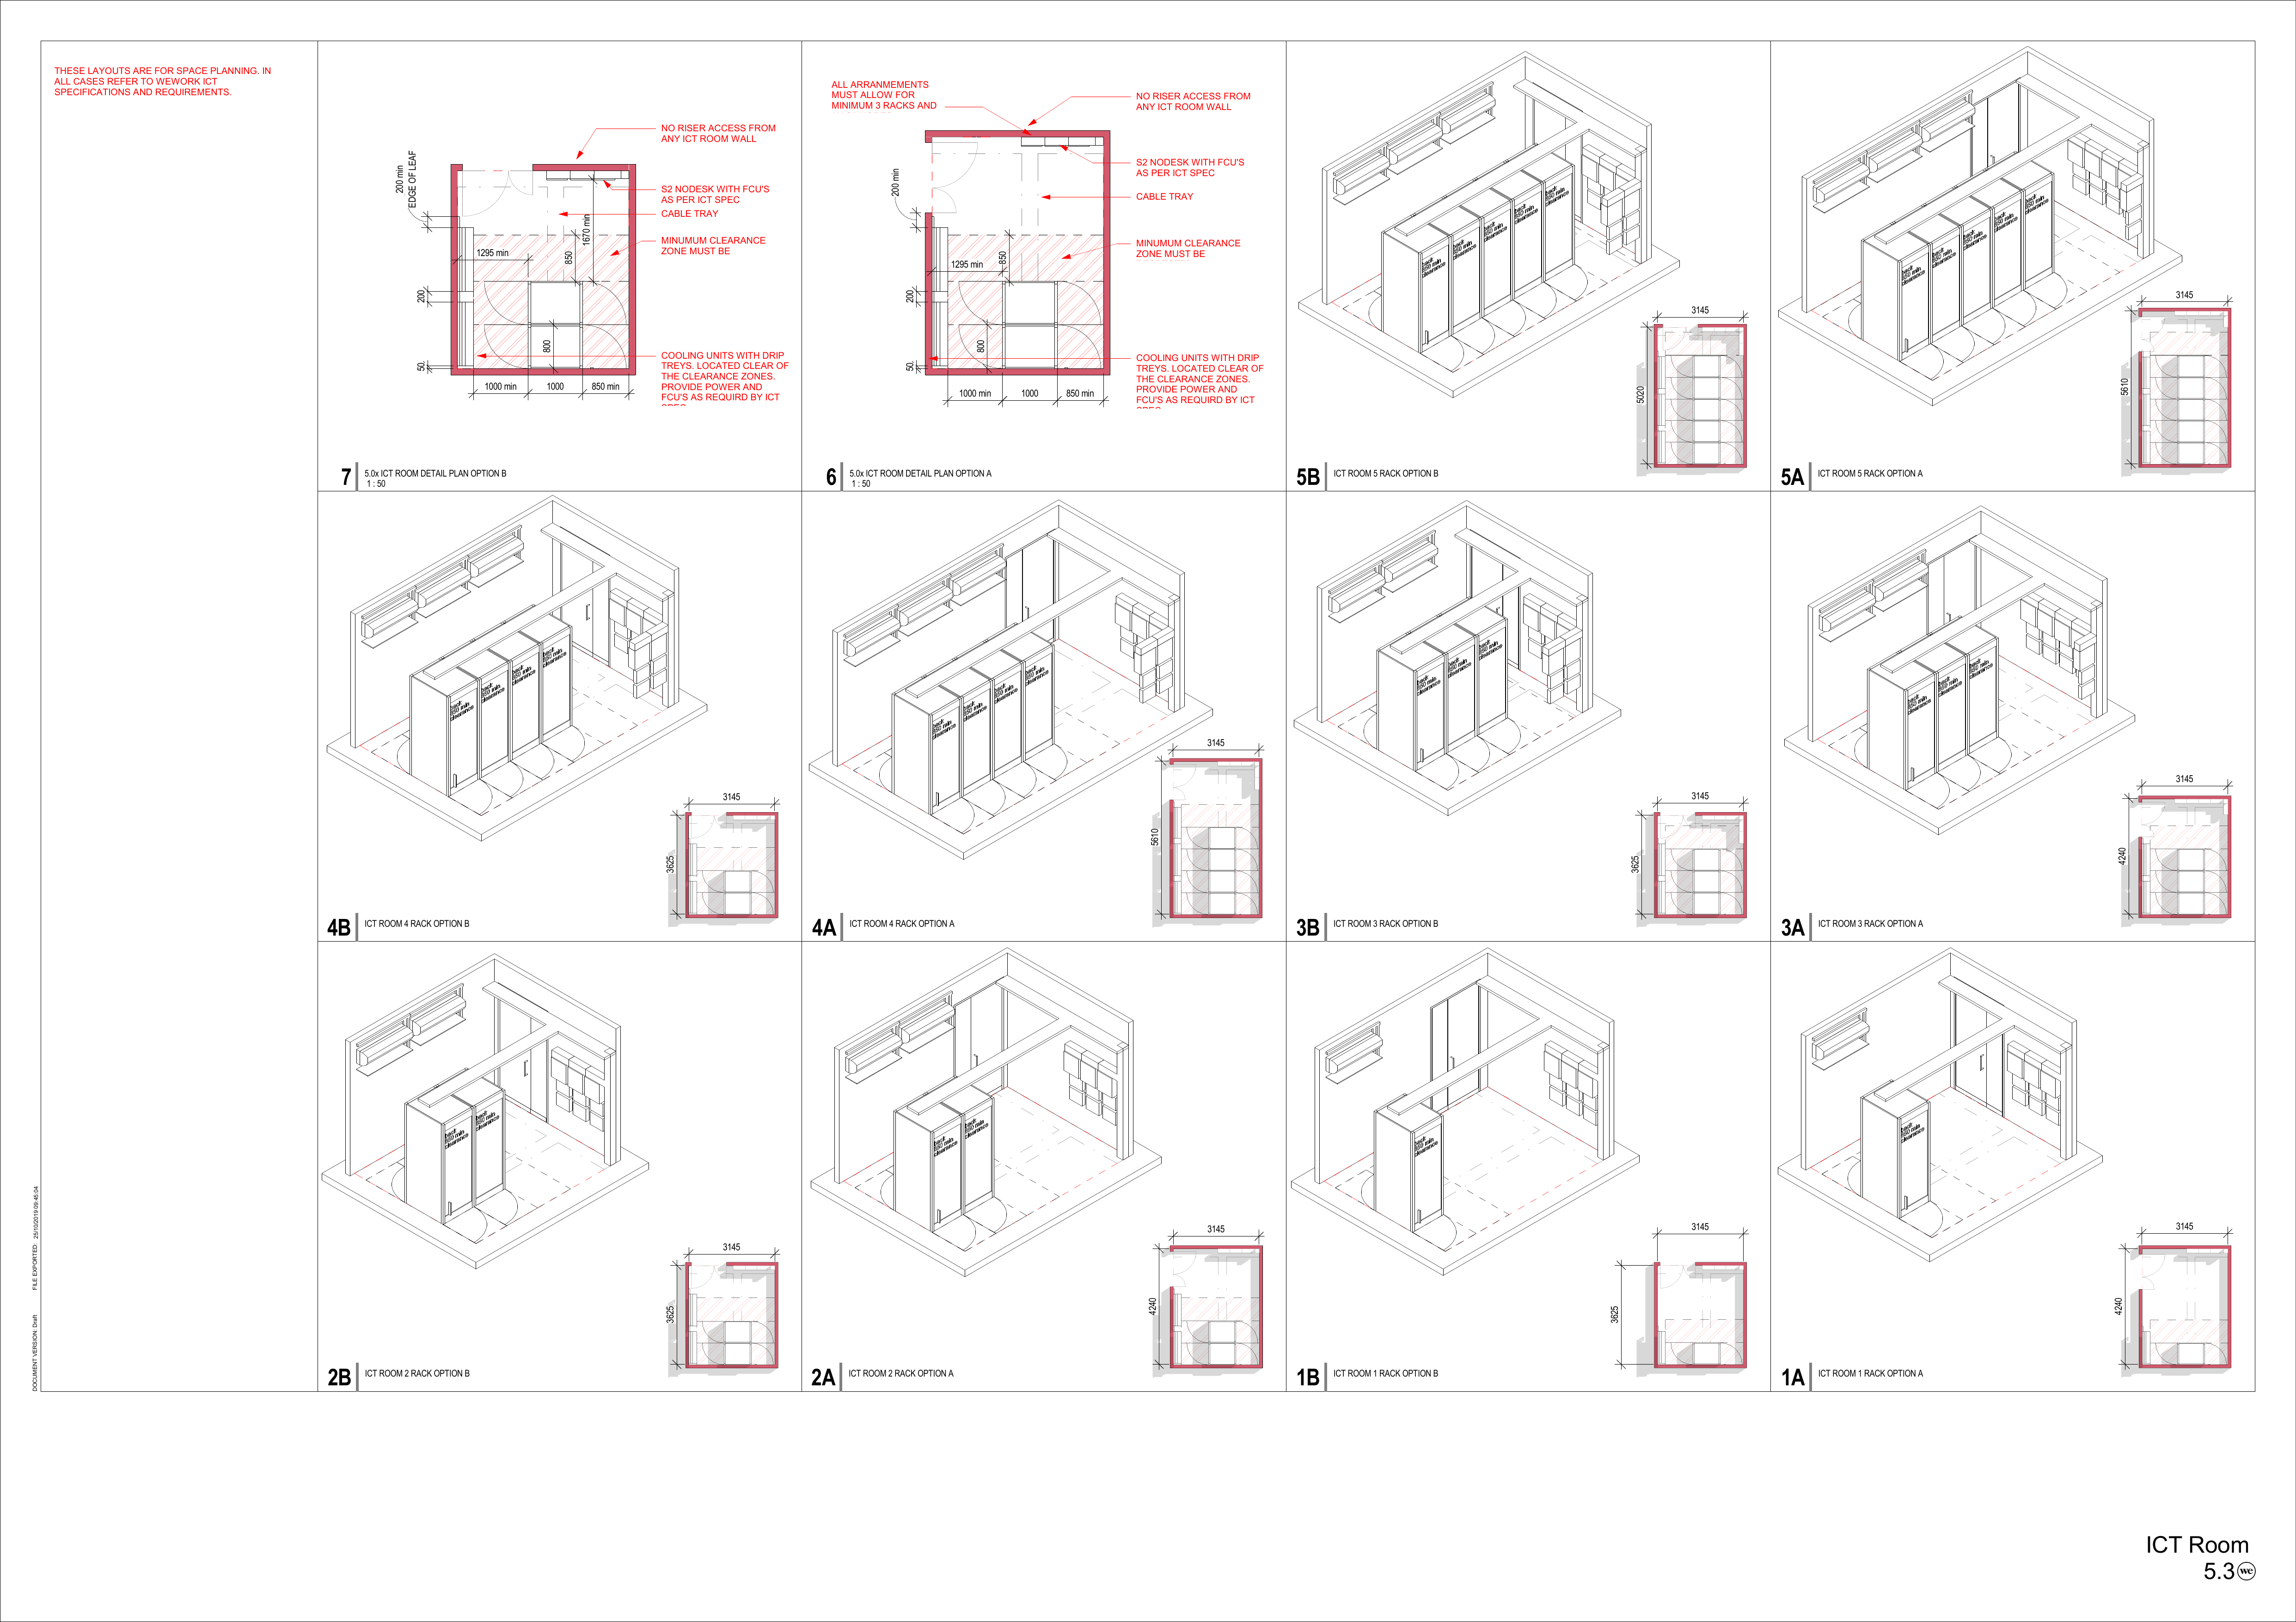
\includegraphics{assets/WeWork/ww_design_standards-30.png}

}

\caption{WeWork\_}

\end{figure}%

\subsection{Pascall + Watson • Building Information Model
Coordinator}\label{pascall-watson-building-information-model-coordinator}

\emph{11/2016 - 07/2018}

\begin{quote}
Pascall+Watson Architects, founded in 1956, is an international
architecture and design firm known for its innovative and sustainable
solutions. With studios across the UK, Europe, and the Middle East, they
specialize in diverse sectors including aviation, education, healthcare,
and leisure. Their collaborative approach ensures each project reflects
the client's vision, creating impactful spaces that serve communities.
Pascall+Watson is committed to environmental and social responsibility,
continually pushing the boundaries of what's possible in architecture
and design.
\end{quote}

Due to the confidential nature of this project, information shared here
is limited to what is publicly available.

\subsubsection{Addressing the Uniquely Challenging Nature of London City
Airport}\label{addressing-the-uniquely-challenging-nature-of-london-city-airport}

London City Airport stands out as a uniquely challenging site and
project for several reasons:

\begin{enumerate}
\def\labelenumi{\arabic{enumi}.}
\tightlist
\item
  \textbf{Location Constraints}:

  \begin{itemize}
  \tightlist
  \item
    \textbf{Urban Setting}: Located in the heart of London, the airport
    is surrounded by residential and commercial buildings. This urban
    setting imposes strict noise and height restrictions, demanding
    innovative design and operational strategies.
  \item
    \textbf{Limited Space}: The airport is built on a relatively small
    footprint compared to other major airports. This limitation requires
    efficient space utilization for runways, taxiways, terminals, and
    other facilities.
  \end{itemize}
\item
  \textbf{Operational Complexity}:

  \begin{itemize}
  \tightlist
  \item
    \textbf{Short Runway}: The airport has one of the shortest
    commercial runways in the world, at just 1,508 meters (4,948 feet).
    This necessitates precise and careful landing and takeoff
    procedures, often requiring aircraft modifications and specialized
    pilot training.
  \end{itemize}
\item
  \textbf{Regulatory and Community Engagement}:

  \begin{itemize}
  \tightlist
  \item
    \textbf{Strict Regulations}: Operating within one of the world's
    most regulated airspaces means compliance with numerous aviation,
    safety, and environmental regulations. Navigating these regulations
    while maintaining efficient operations requires meticulous planning
    and execution.
  \item
    \textbf{Community Relations}: The airport must actively engage with
    the local community to address concerns related to noise, traffic,
    and environmental impact. Building and maintaining good relations
    with the community is vital for its ongoing operations and potential
    expansion projects.
  \end{itemize}
\item
  \textbf{Innovative Solutions}:

  \begin{itemize}
  \tightlist
  \item
    \textbf{Technological Advancements}: To address these challenges,
    the airport incorporates state-of-the-art technologies in air
    traffic management, security, and passenger services. Innovations
    such as remote air traffic control towers and biometric boarding
    systems are part of its strategy to enhance efficiency and passenger
    experience.
  \item
    \textbf{Infrastructure Upgrades}: Continuous infrastructure upgrades
    are essential to meet growing demand and evolving regulatory
    standards. Projects like terminal expansions, runway enhancements,
    and improved transportation links are critical to maintaining the
    airport's competitive edge.
  \end{itemize}
\end{enumerate}

\begin{figure}[H]

{\centering 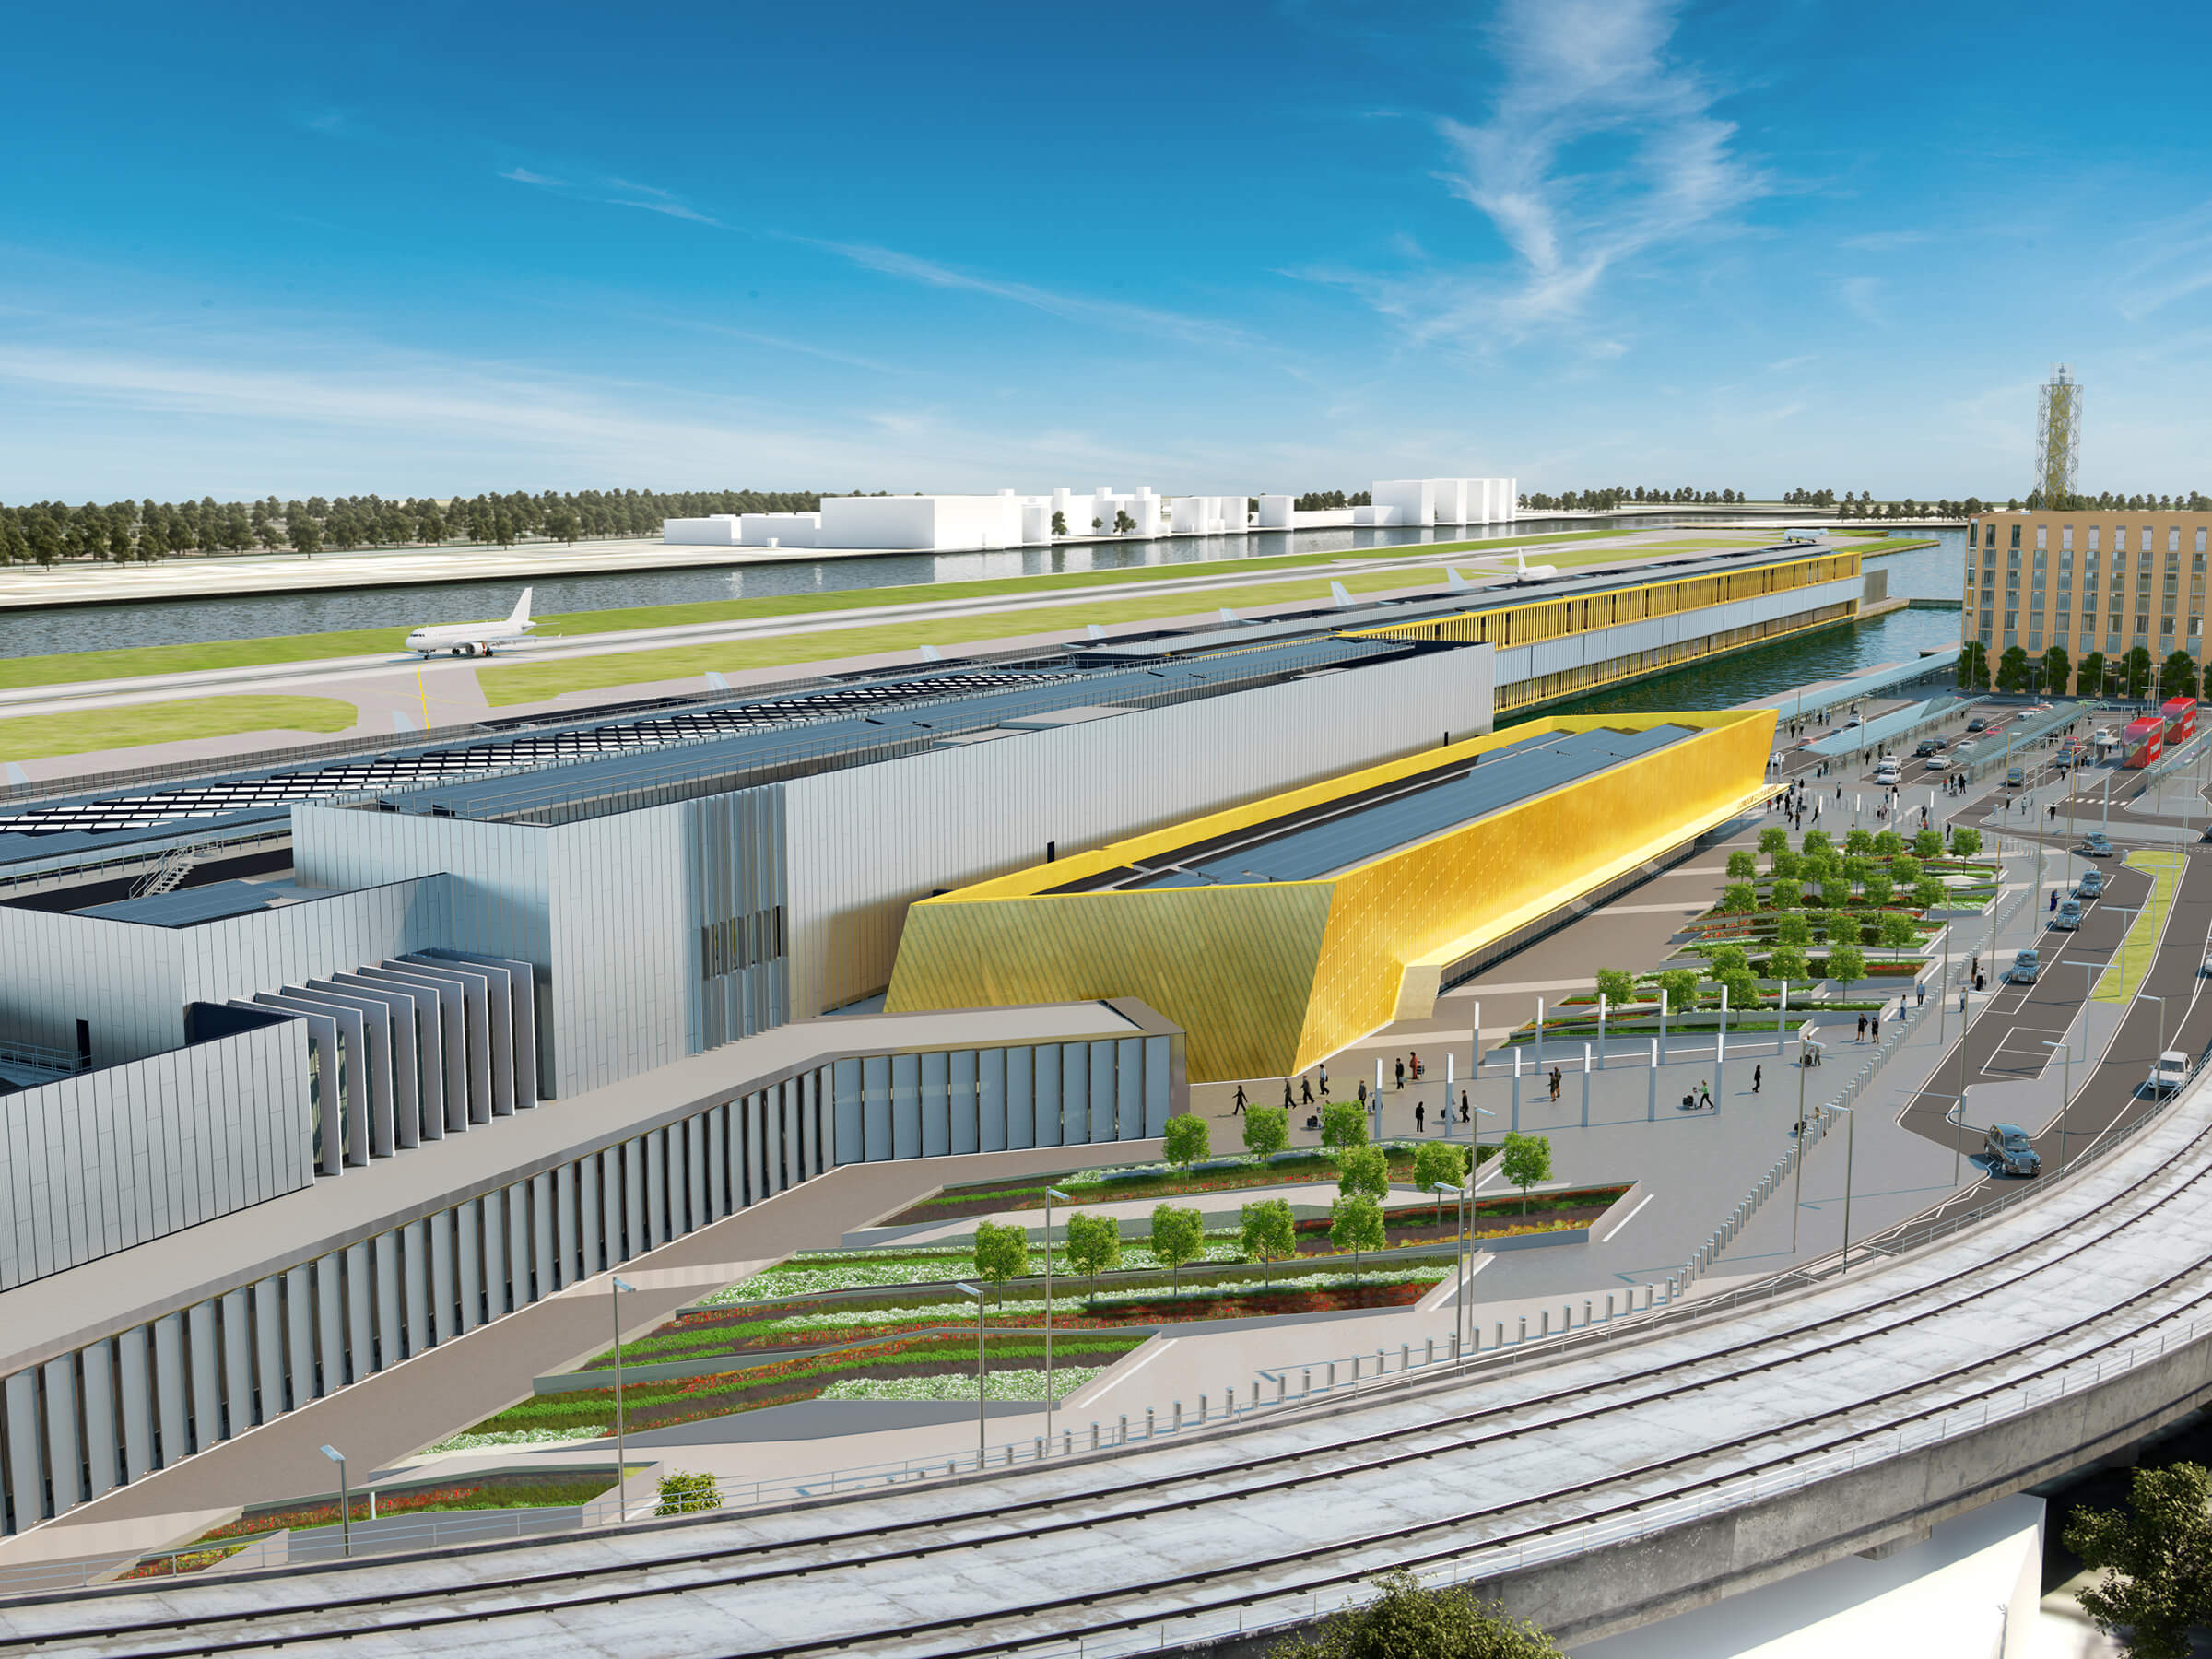
\includegraphics{assets/PAW/London-City-Airport-Pascall-Watson-(1).jpg}

}

\caption{model overview}

\end{figure}%%
\begin{figure}[H]

{\centering 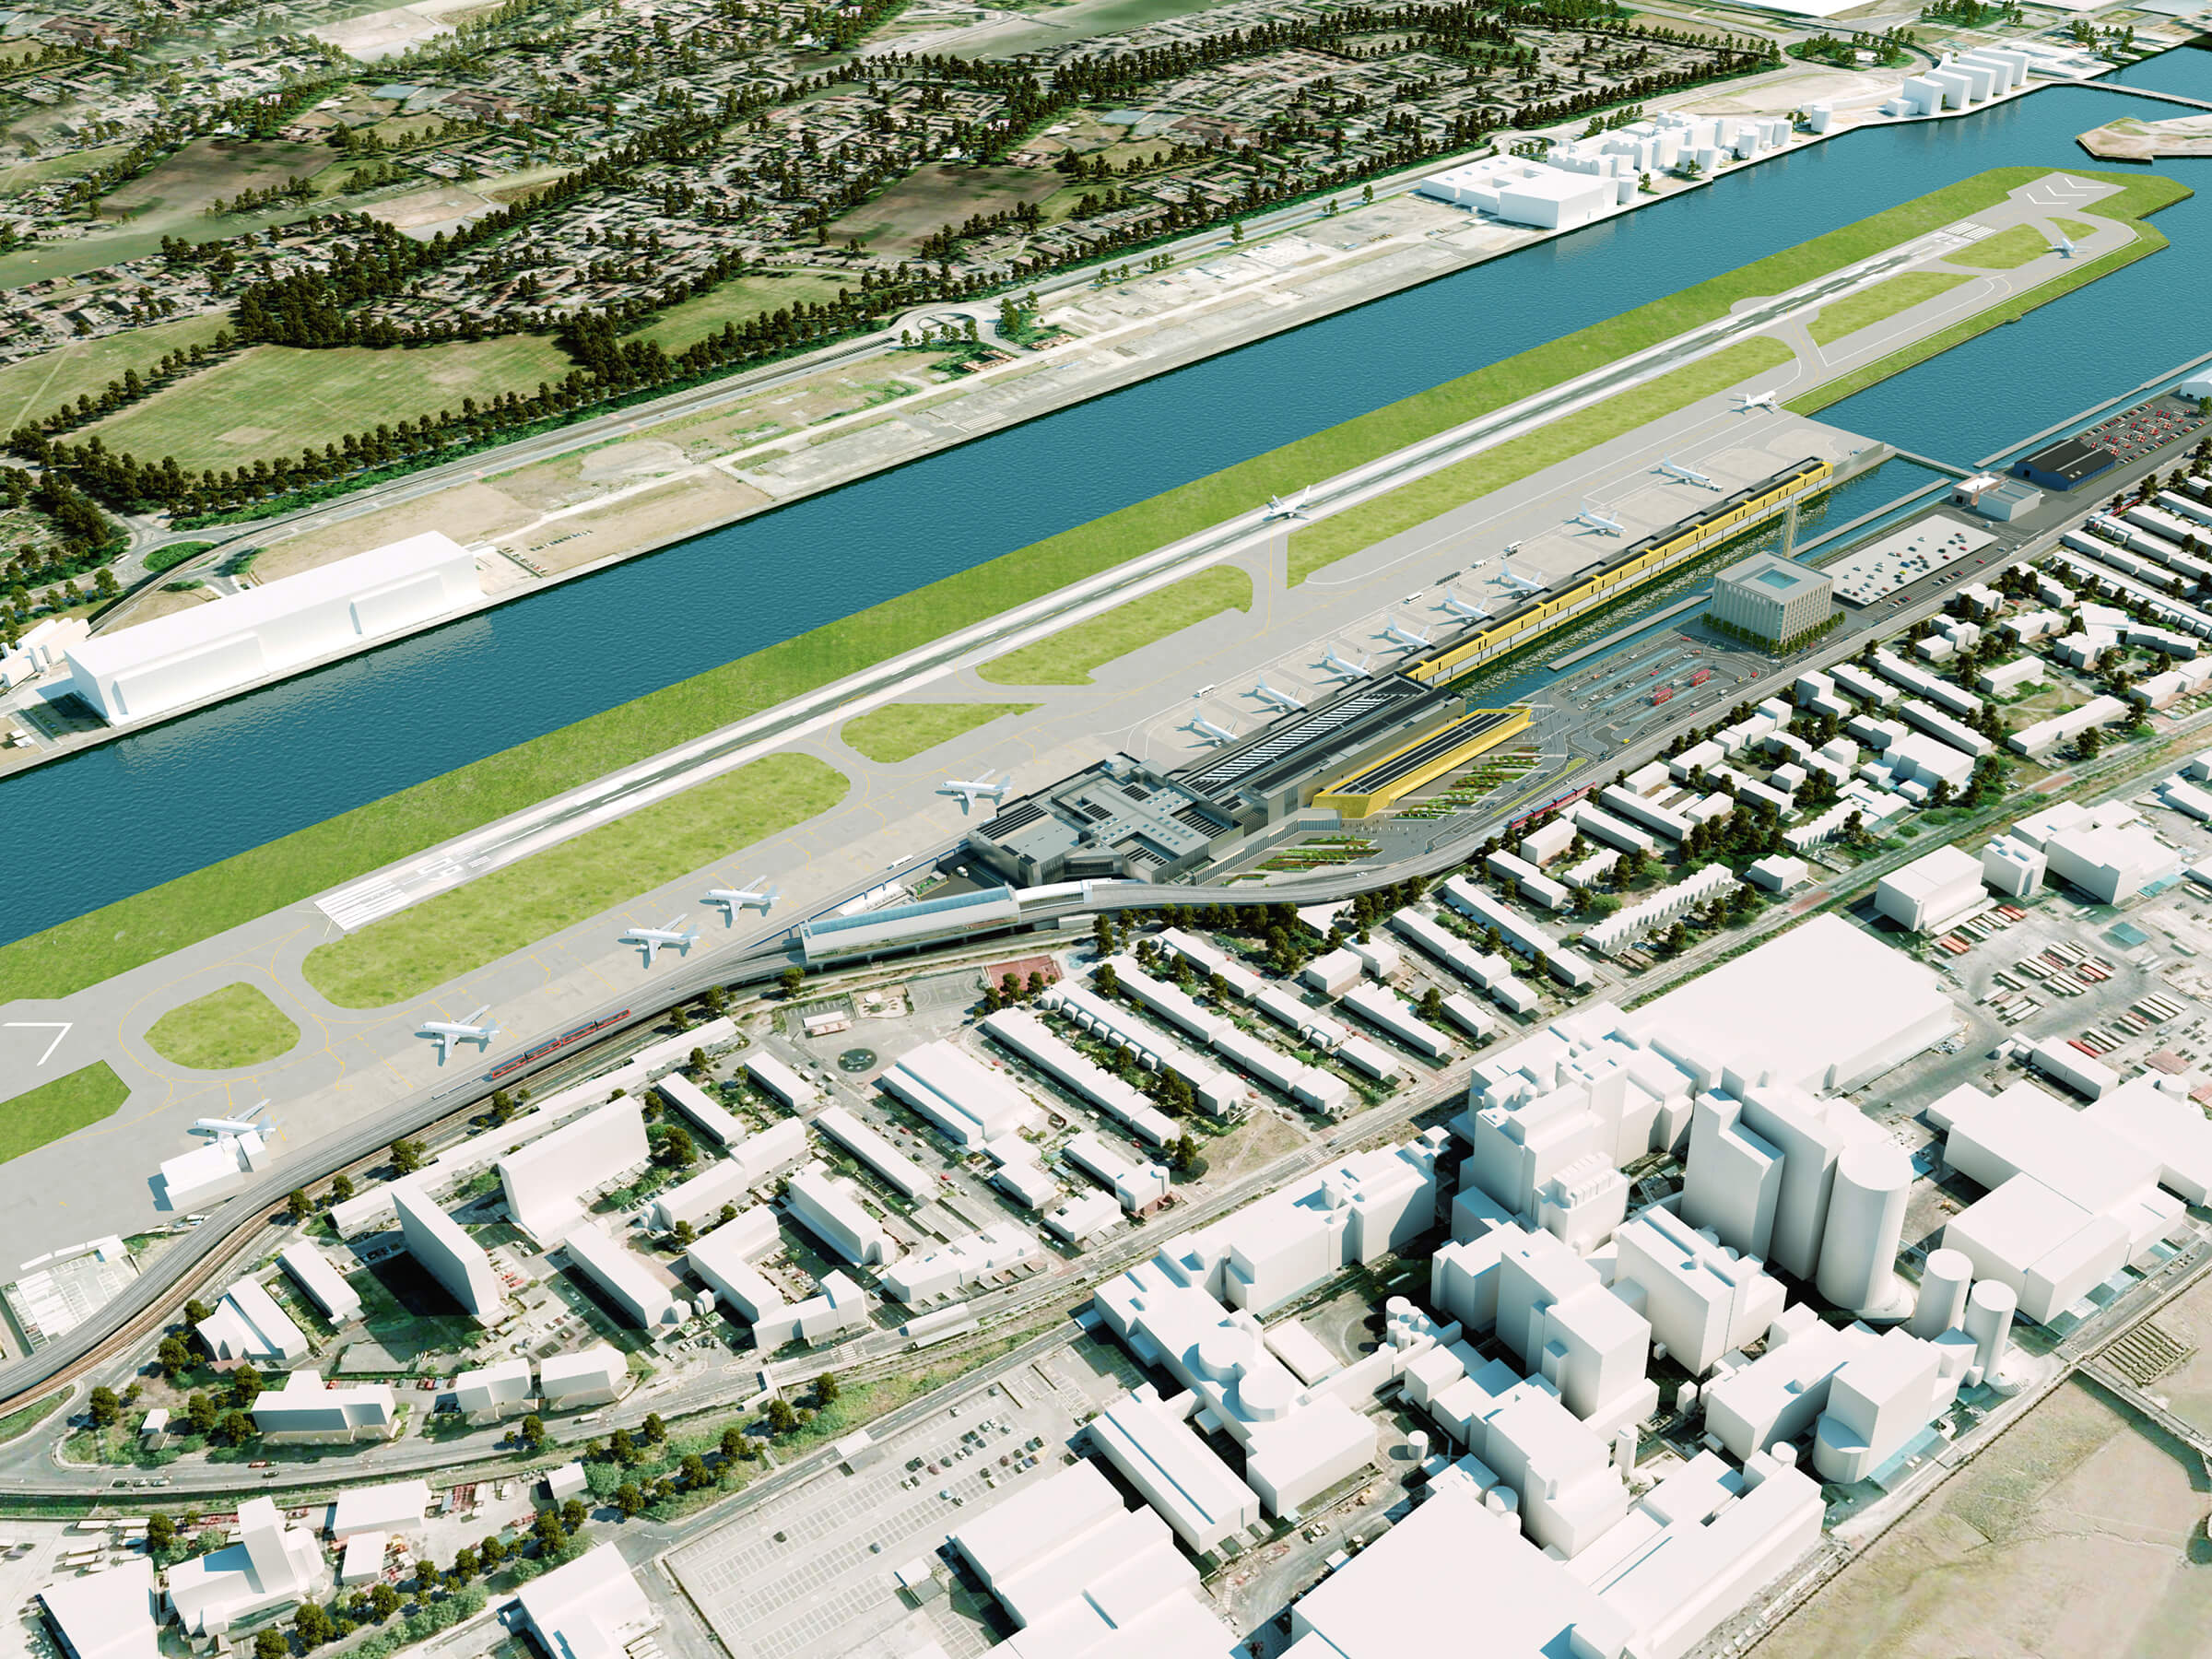
\includegraphics{assets/PAW/London-City-Airport-Pascall-Watson.jpg}

}

\caption{model overview}

\end{figure}%%
\begin{figure}[H]

{\centering 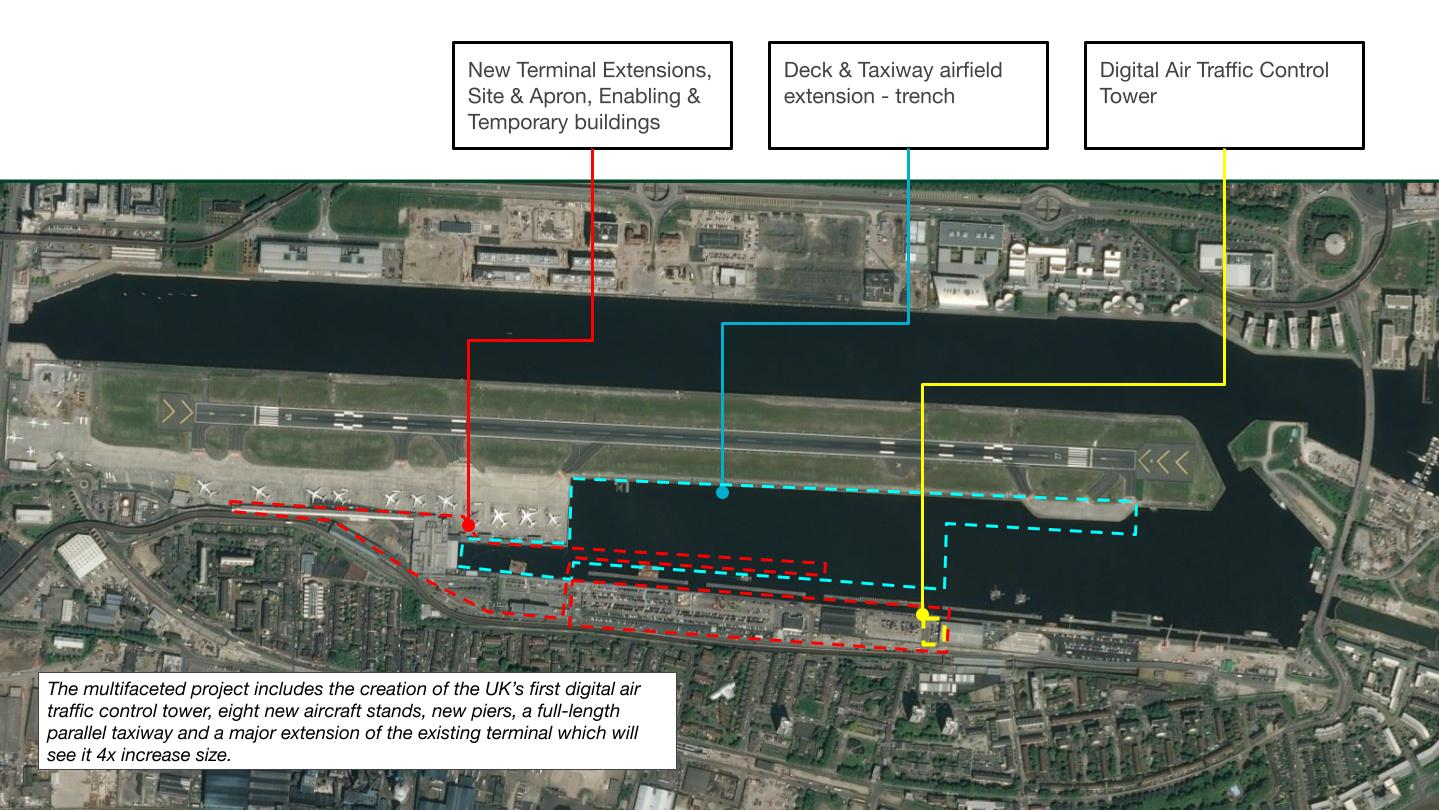
\includegraphics{assets/PAW/2020-Portfolio-Google-Overview.jpg}

}

\caption{model overview}

\end{figure}%

\subsubsection{Coordination and
collaboration}\label{coordination-and-collaboration}

\begin{figure}[H]

{\centering 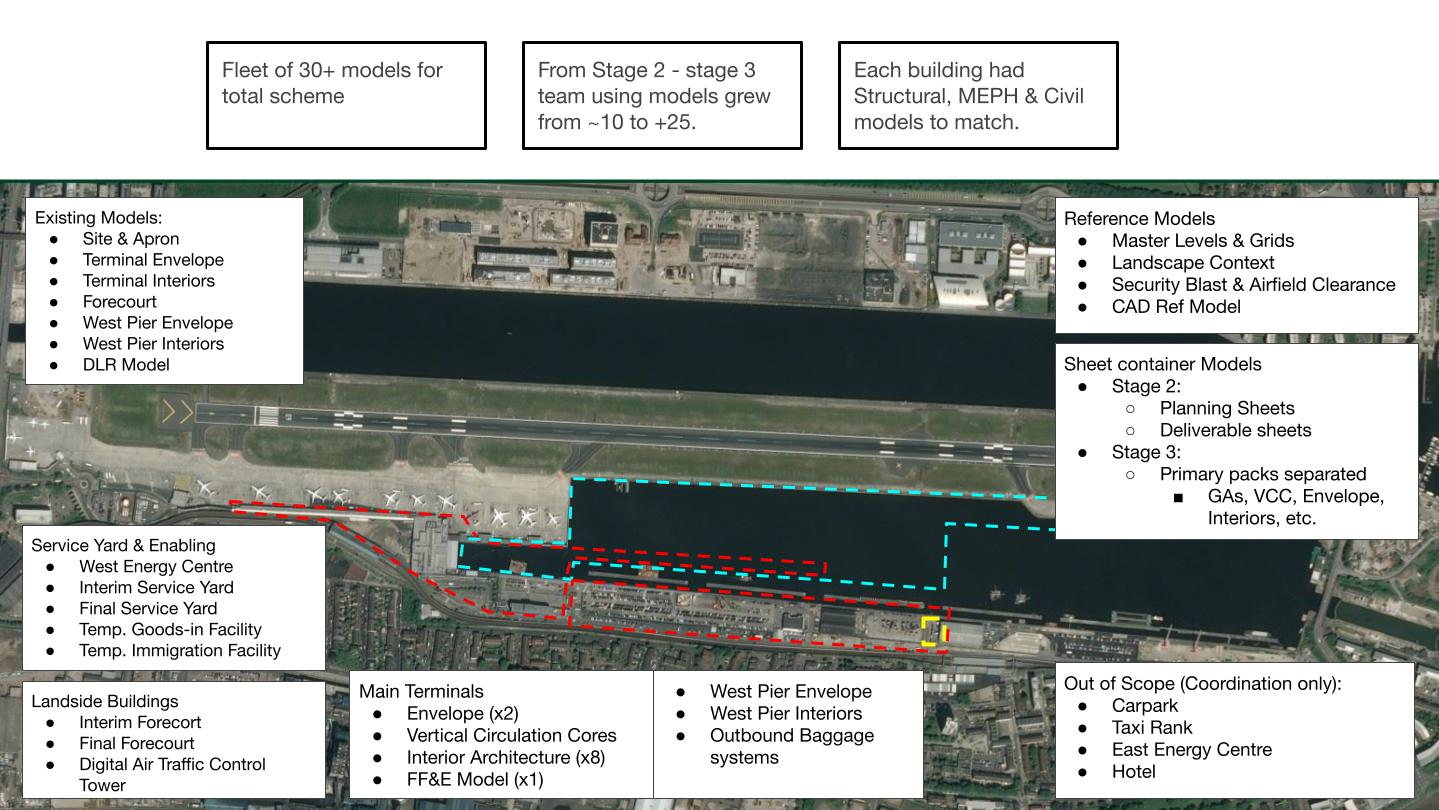
\includegraphics{assets/PAW/LCY-modelBreakdown.jpg}

}

\caption{modelBreakdown}

\end{figure}%%
\begin{figure}[H]

{\centering 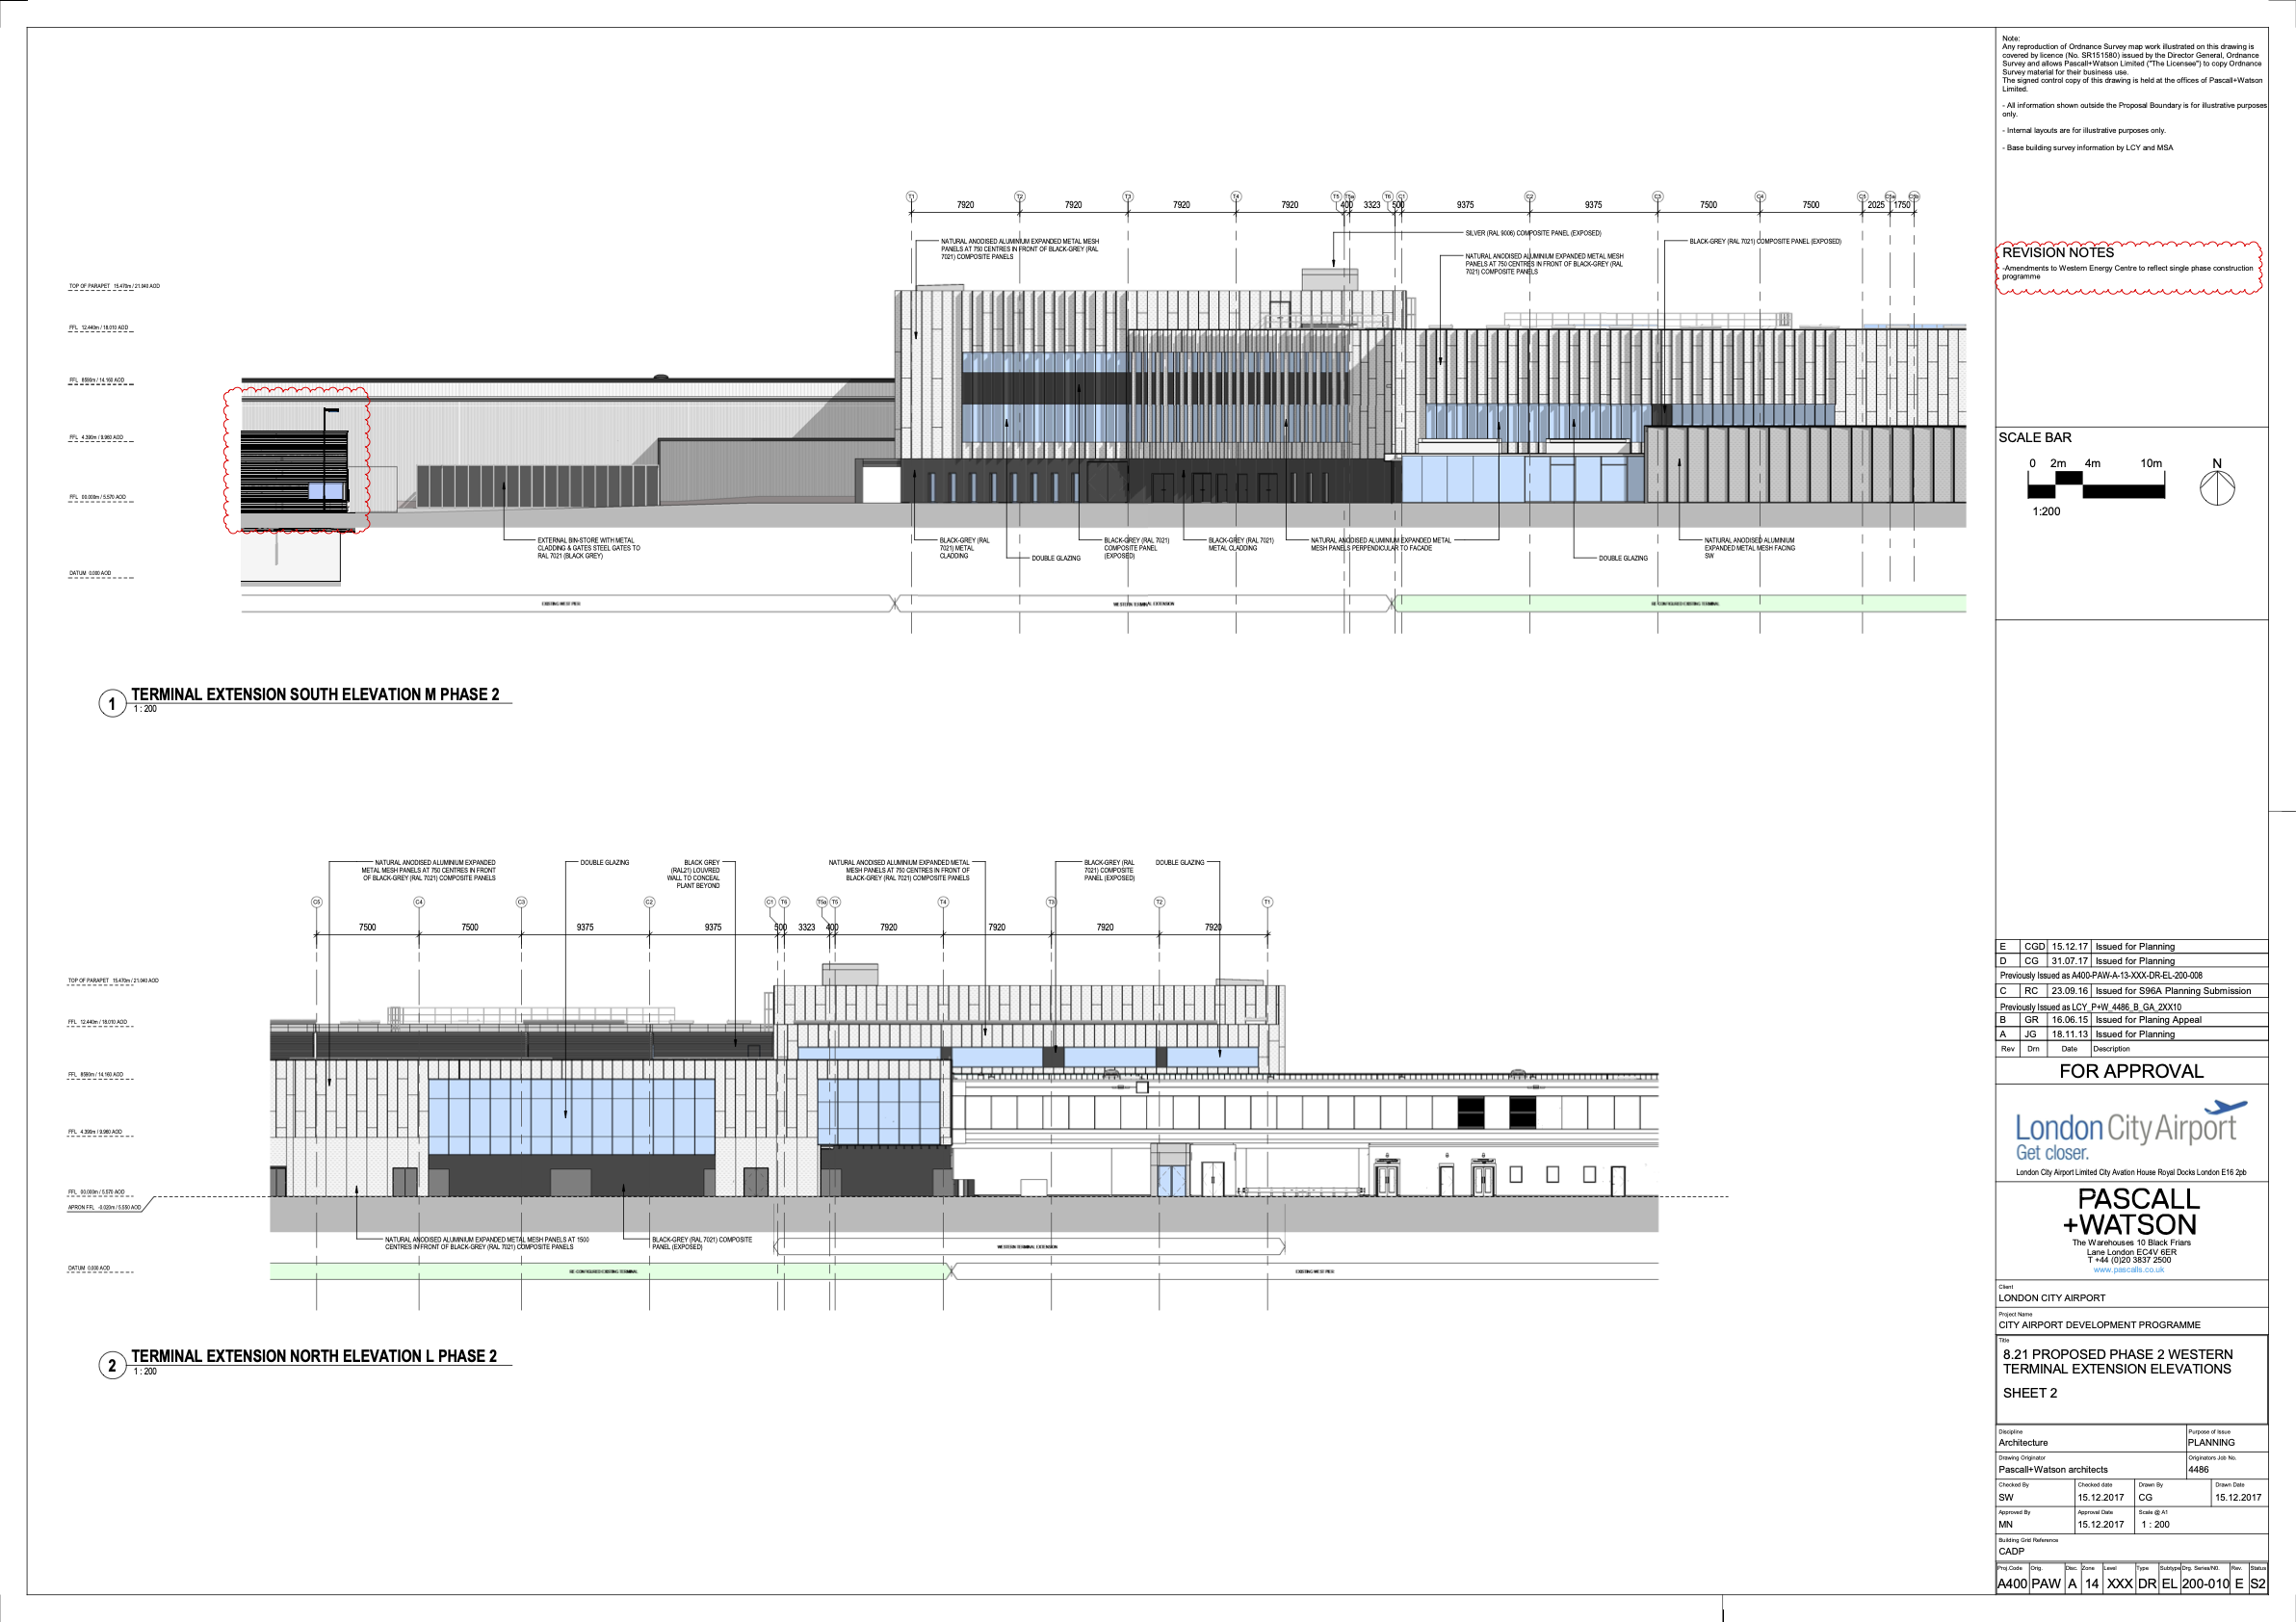
\includegraphics{assets/PAW/Proposed-Phase-2-Extension-Elevations.png}

}

\caption{PAW-LCA-planning-plans}

\end{figure}%%
\begin{figure}[H]

{\centering 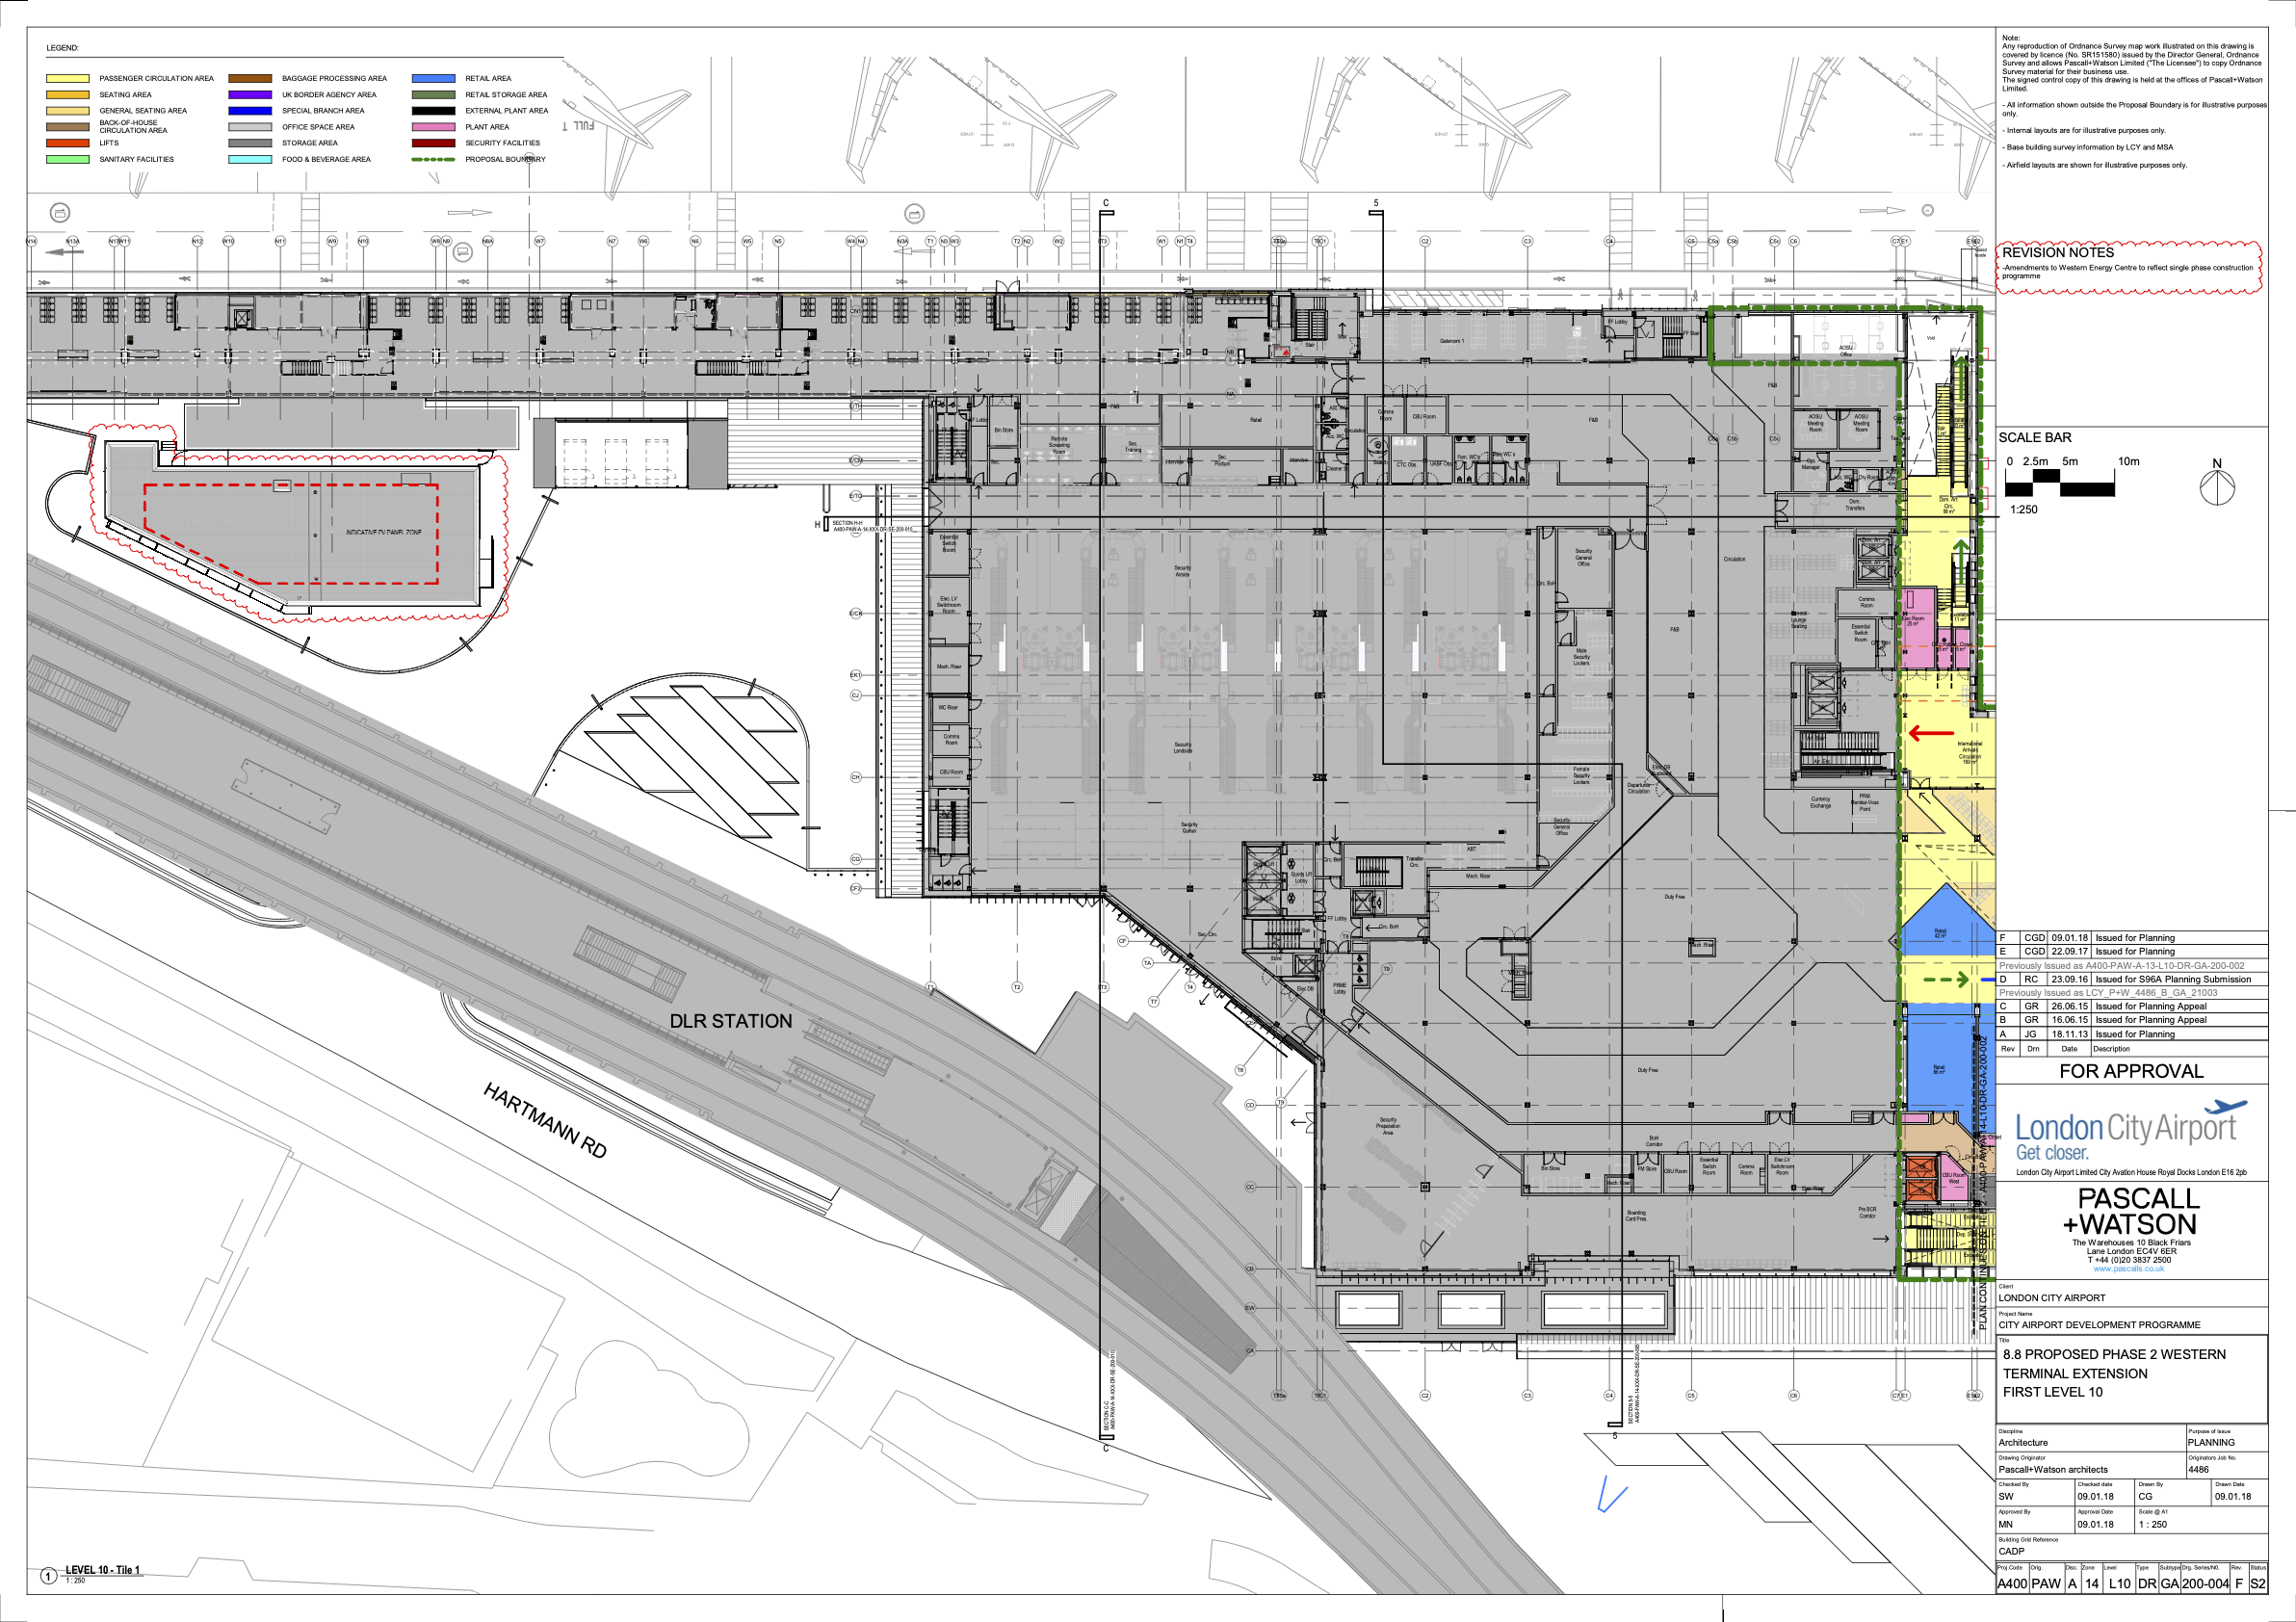
\includegraphics{assets/PAW/Proposed-Phase-2-Terminal-Extension-First-Level.png}

}

\caption{PAW-LCA-planning-plans}

\end{figure}%%
\begin{figure}[H]

{\centering 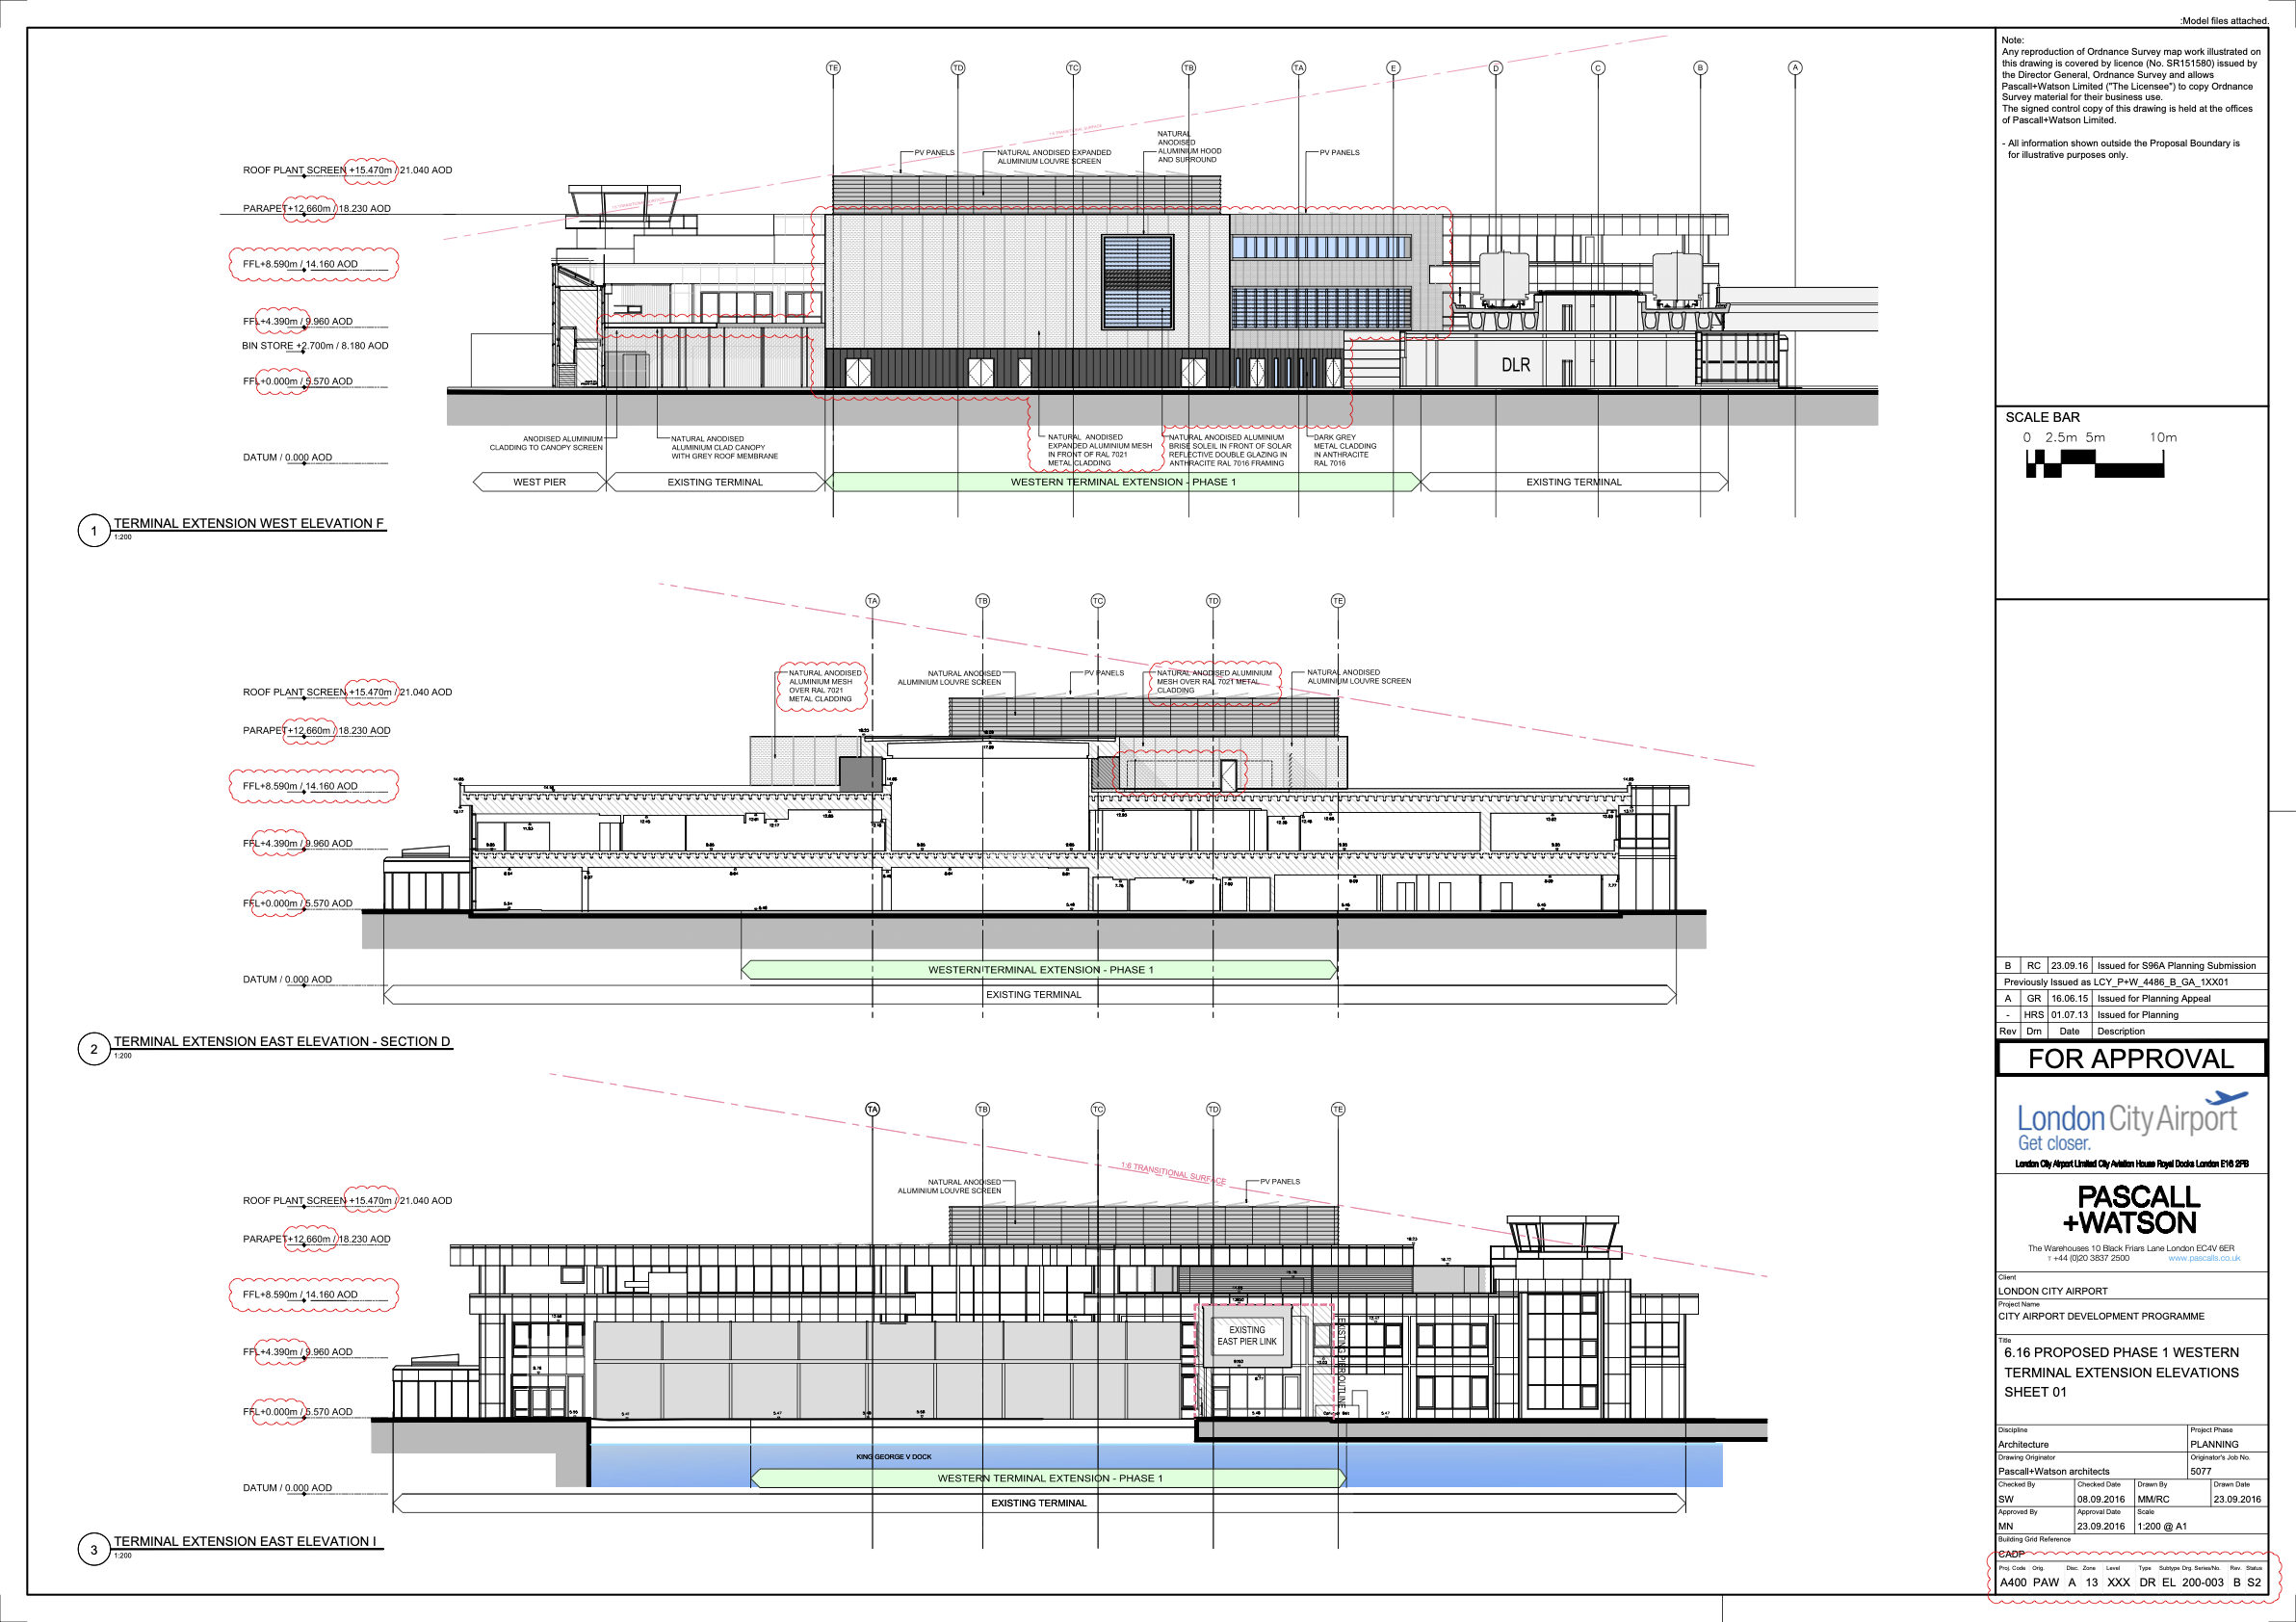
\includegraphics{assets/PAW/Western-Terminal-Extension-Elevations.png}

}

\caption{PAW-LCA-planning-plans}

\end{figure}%

\subsubsection{Digital Air Traffic Control
Tower}\label{digital-air-traffic-control-tower}

\href{https://www.pascalls.co.uk/news/article/pascallwatsons-remote-air-traffic-control-tower-is-world-first-for-a-major-international-airport/}{Pascall+Watson's
remote air traffic control tower is world-first for a major
international airport} \textgreater{} London City Airport has introduced
the UK's first digital air traffic control tower, a significant
development in its £400 million redevelopment program. This
state-of-the-art tower allows controllers to manage air traffic remotely
using high-definition cameras and sensors, providing a 360-degree view
of the airfield from a control center located over 70 miles away. This
innovative approach enhances operational efficiency and safety, marking
a transformative step in airport technology
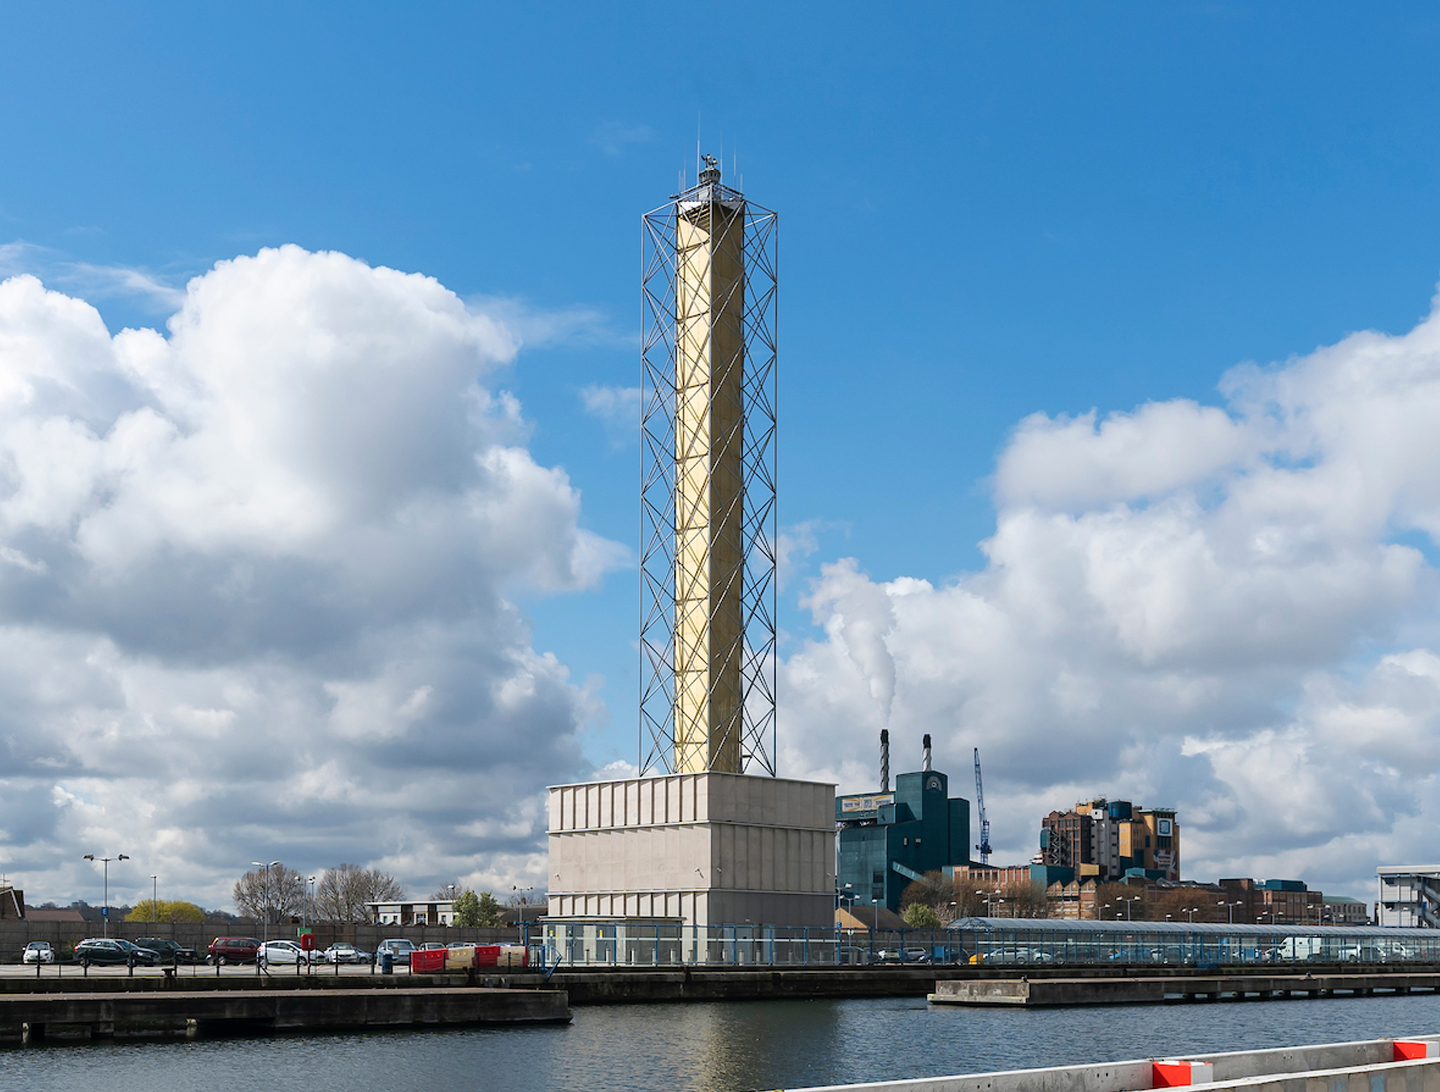
\includegraphics{assets/PAW/LCY2-News-4-3.jpg}

\subsubsection{BIM Coordination}\label{bim-coordination}

\begin{figure}[H]

{\centering 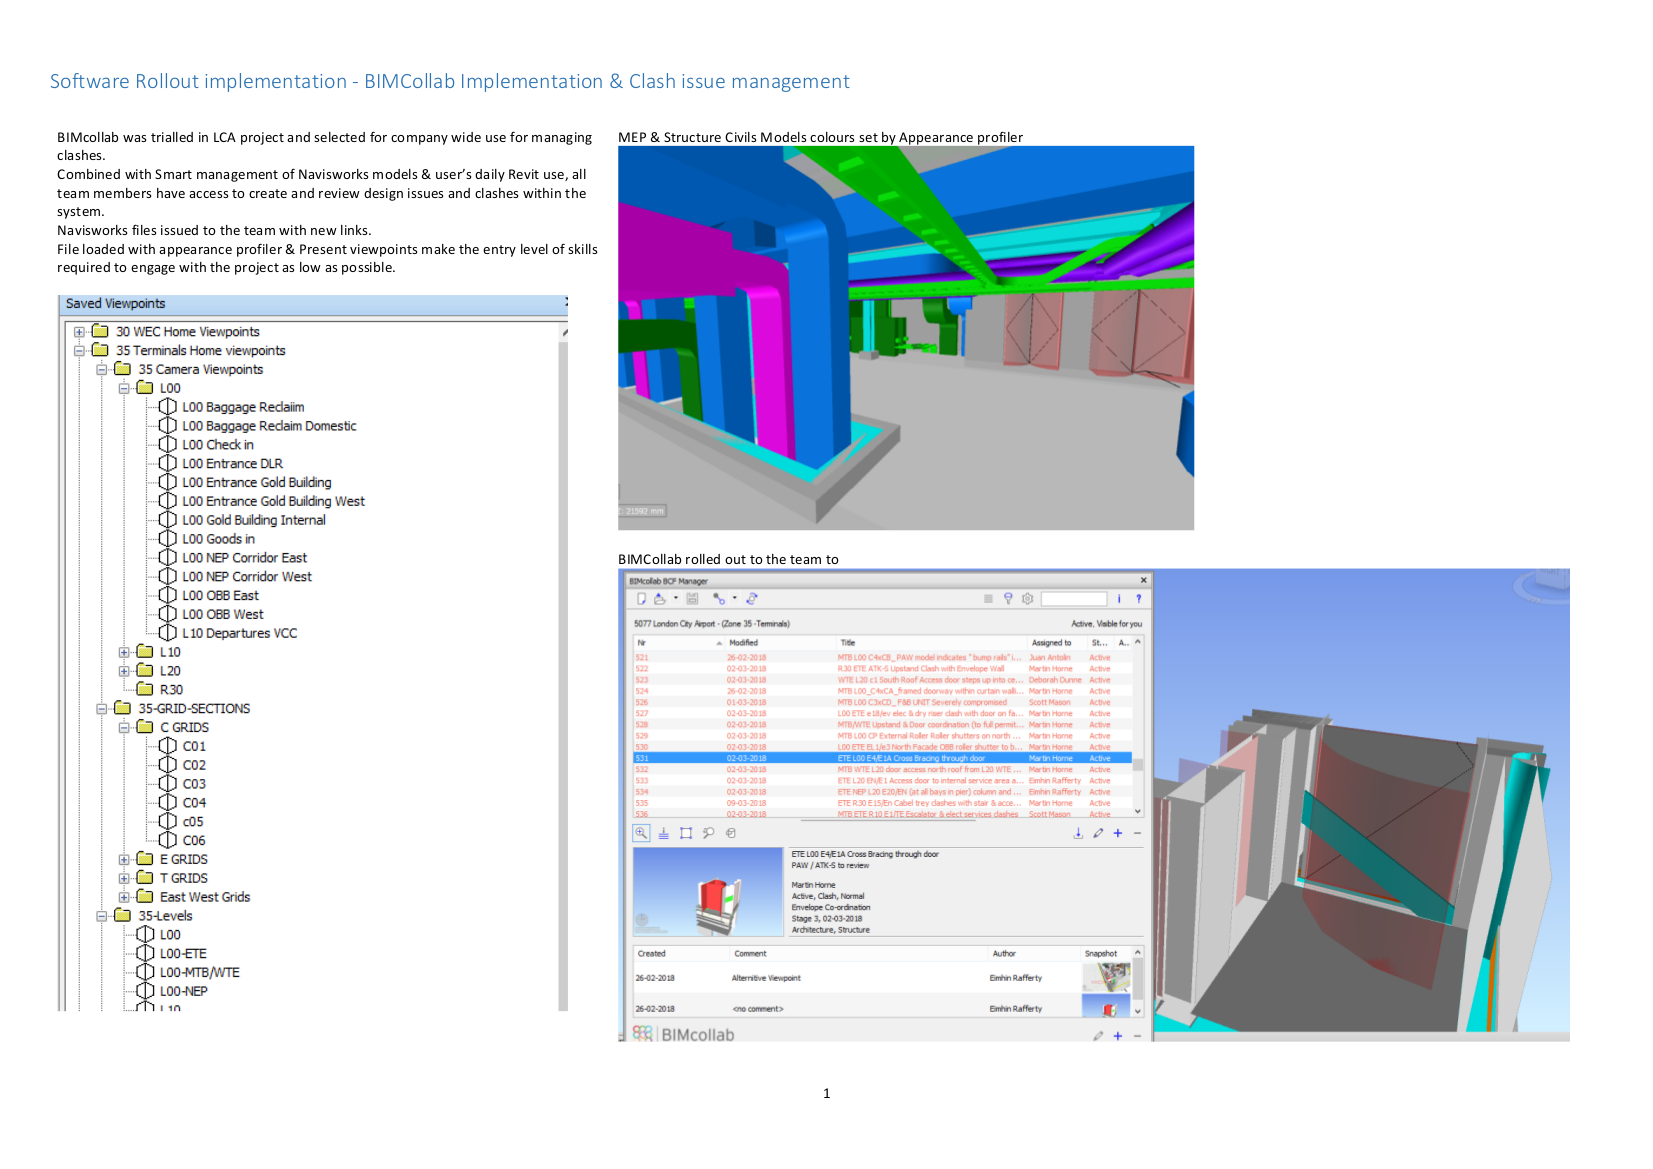
\includegraphics{assets/PAW/P+W-BIMcollab-1.png}

}

\caption{PAW\_coord\_collab}

\end{figure}%%
\begin{figure}[H]

{\centering 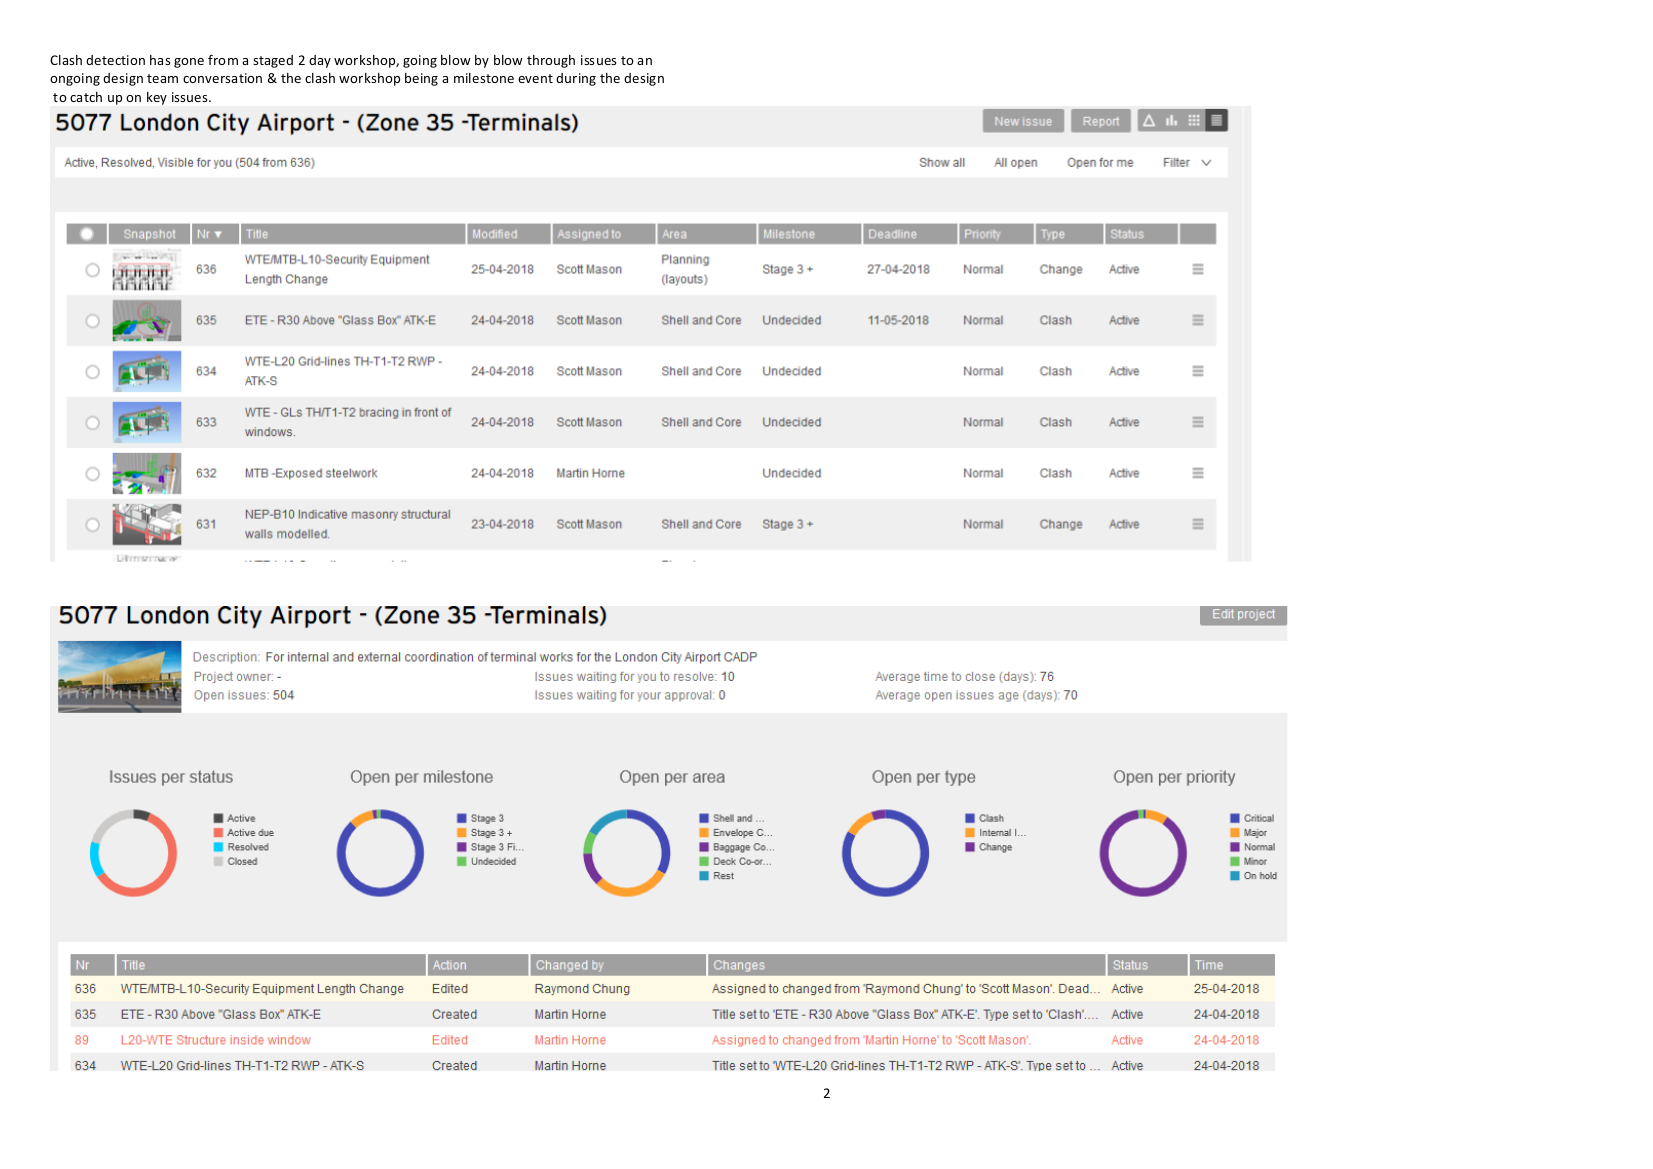
\includegraphics{assets/PAW/P+W-BIMcollab-2.png}

}

\caption{PAW\_coord\_collab}

\end{figure}%%
\begin{figure}[H]

{\centering 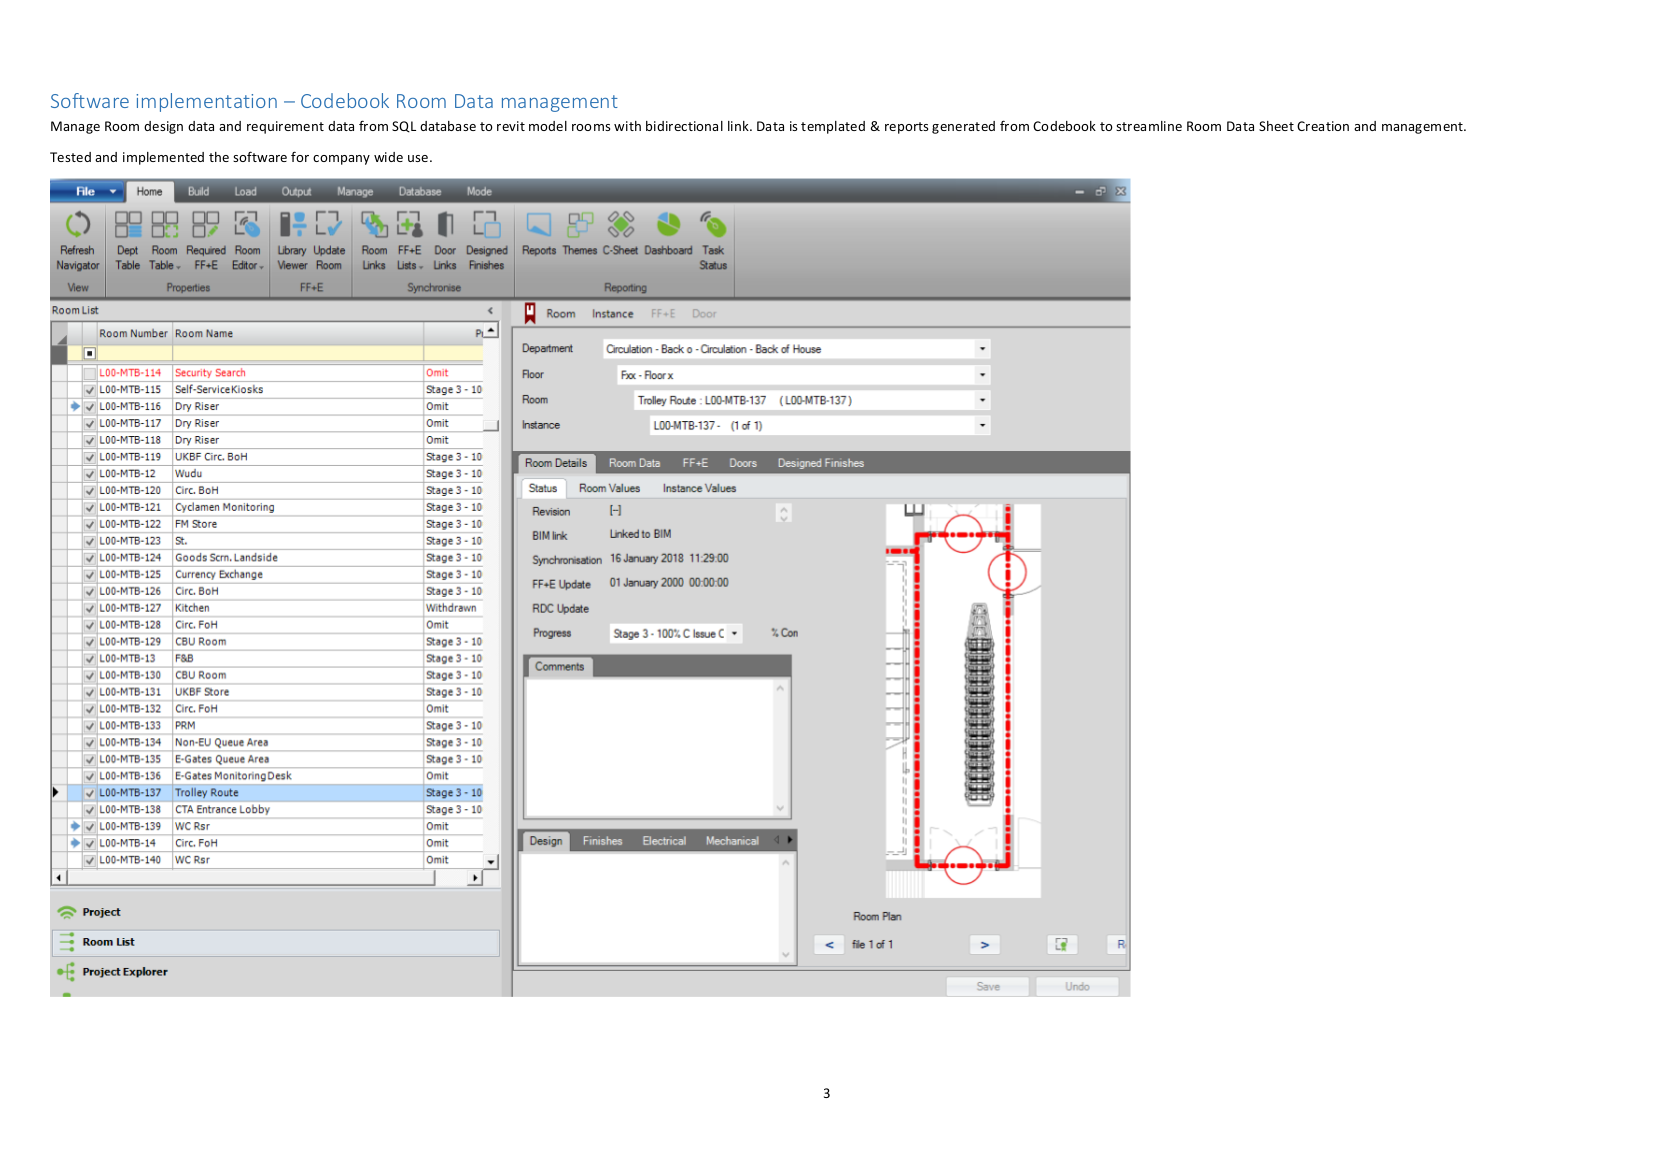
\includegraphics{assets/PAW/P+W-BIMcollab-3.png}

}

\caption{PAW\_coord\_collab}

\end{figure}%

\subsubsection{Delivering Classifications, COBie and Efficncies with
Dynamo}\label{delivering-classifications-cobie-and-efficncies-with-dynamo}

\begin{figure}[H]

{\centering 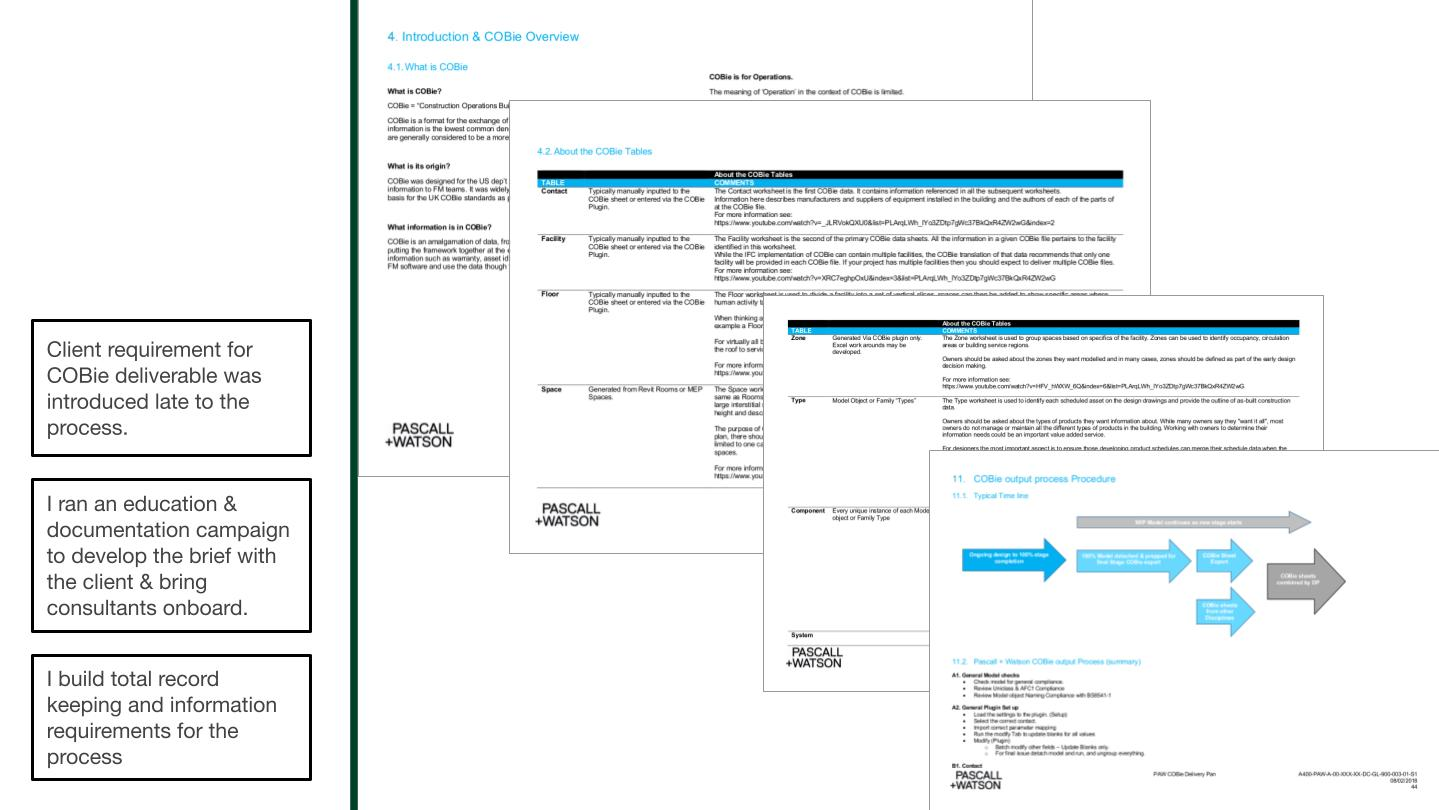
\includegraphics{assets/PAW/2020-Portfolio-Google-Slides-data.jpg}

}

\caption{PAW-Data-Code}

\end{figure}%%
\begin{figure}[H]

{\centering 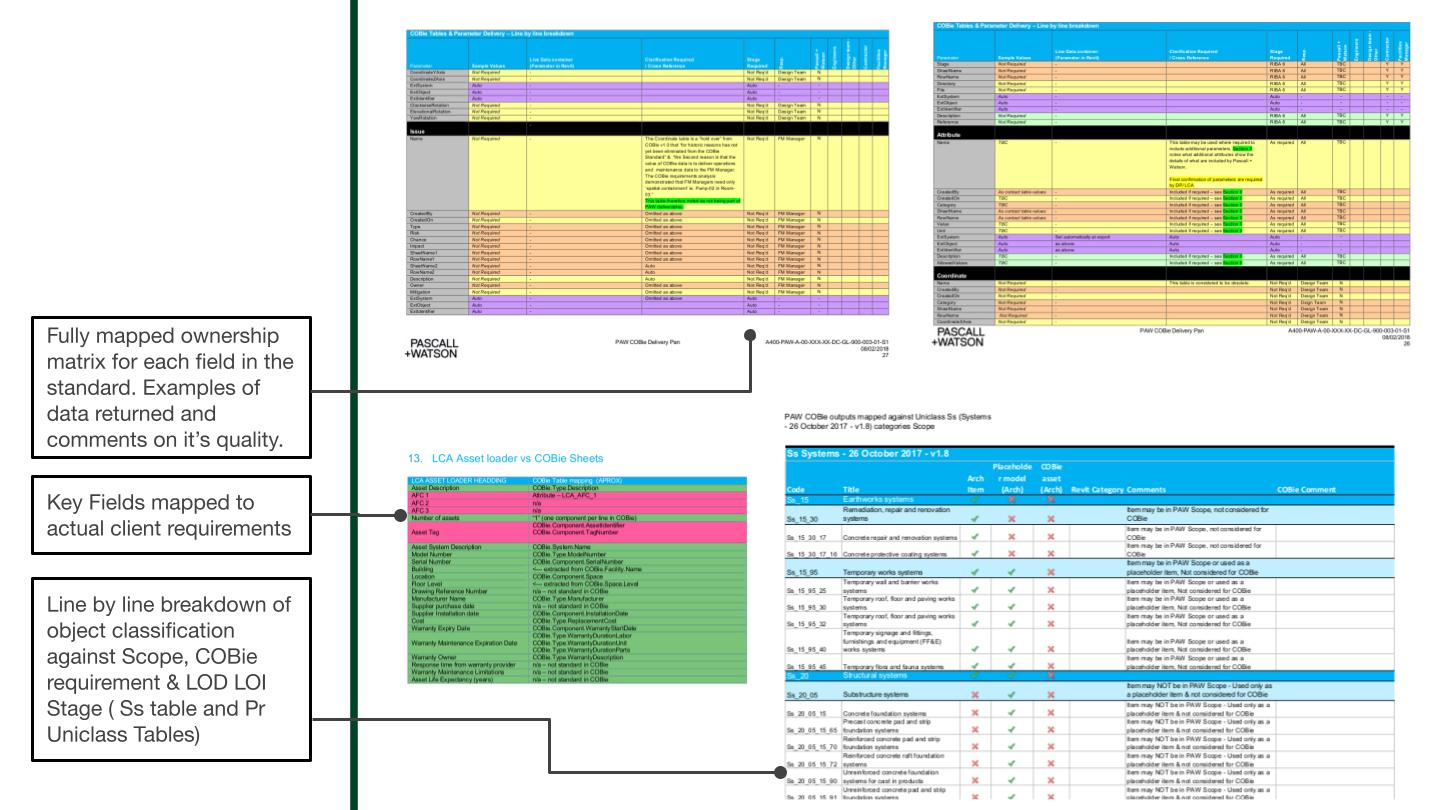
\includegraphics{assets/PAW/2020-Portfolio-Google-Slides-data2.jpg}

}

\caption{PAW-Data-Code}

\end{figure}%%
\begin{figure}[H]

{\centering 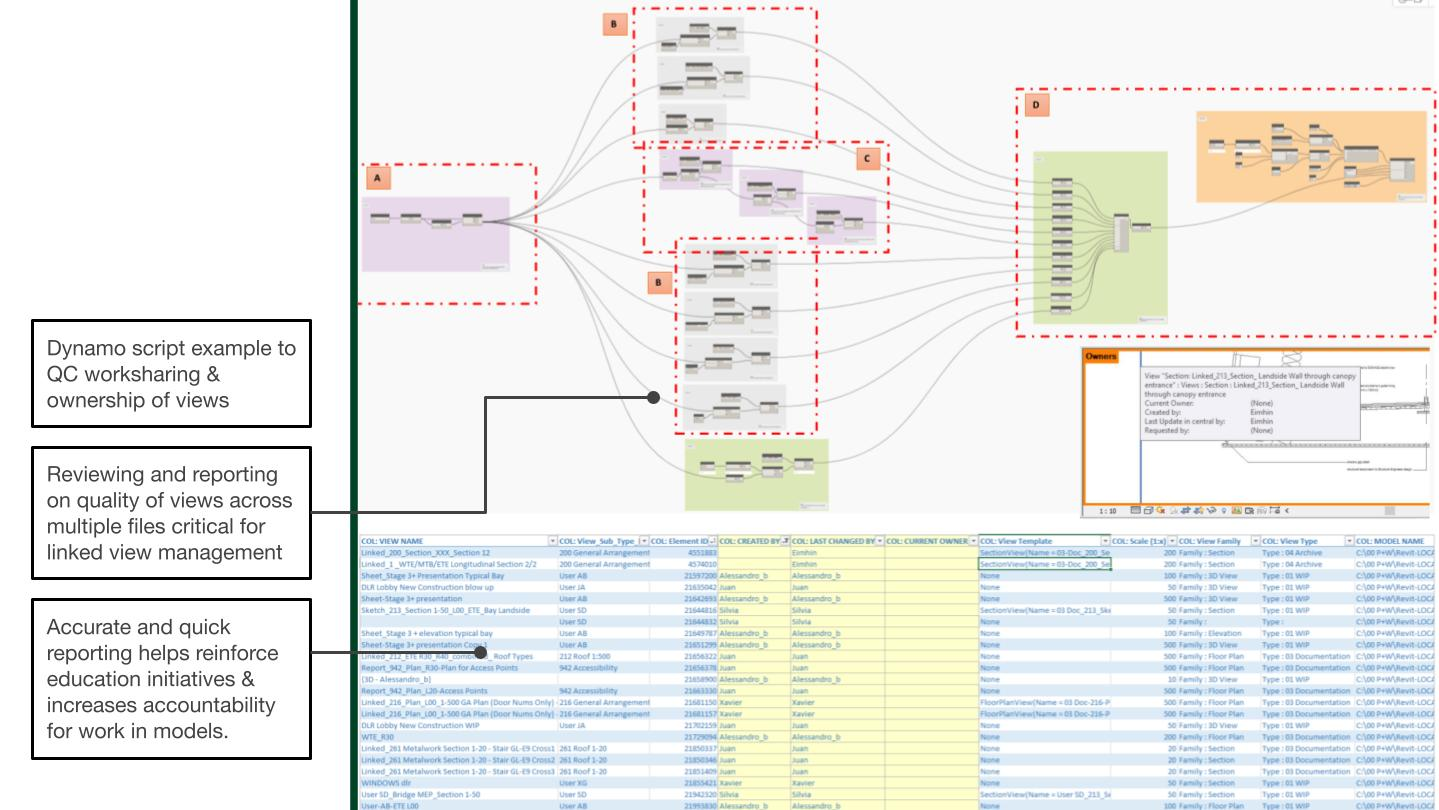
\includegraphics{assets/PAW/2020-Portfolio-Google-Slides-dynamo1.jpg}

}

\caption{PAW-Data-Code}

\end{figure}%%
\begin{figure}[H]

{\centering 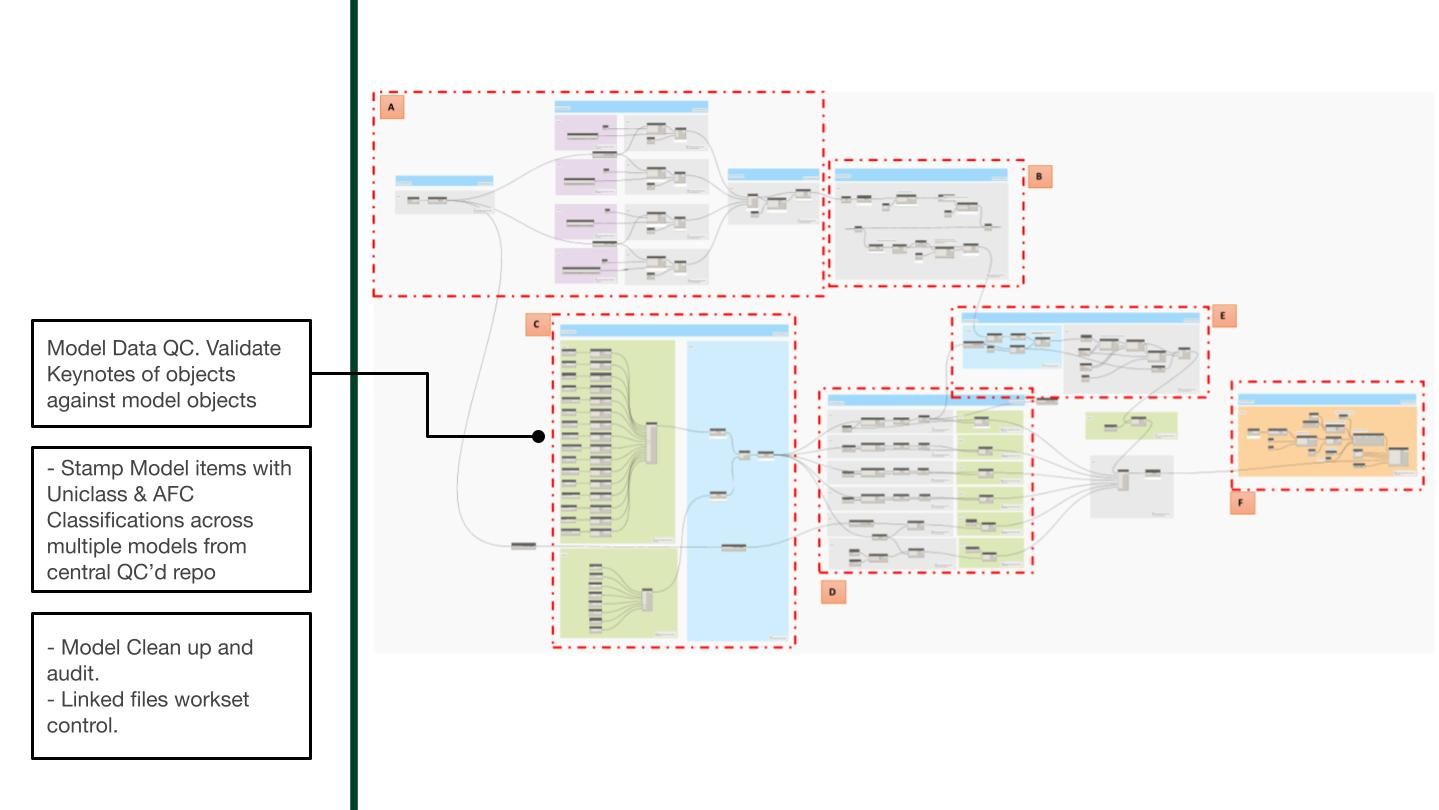
\includegraphics{assets/PAW/2020-Portfolio-Google-Slides-dynamo2.jpg}

}

\caption{PAW-Data-Code}

\end{figure}%

\subsection{Watkins Gray International • Building Information Model
Manager}\label{watkins-gray-international-building-information-model-manager}

\emph{02/2014 - 11/2016} \textgreater{} \textgreater{} Watkins Gray
International LLP is a distinguished architecture and design firm
dedicated to enhancing lives through innovative and sustainable building
solutions. Specializing in sectors such as education, healthcare,
residential, commercial, and defense, their expertise spans diverse
project types. Committed to the art and science of building, Watkins
Gray International LLP combines creativity with technical precision to
deliver transformative spaces that meet the evolving needs of clients.

\subsubsection{Seven Kings Redbridge}\label{seven-kings-redbridge}

\begin{figure}[H]

{\centering 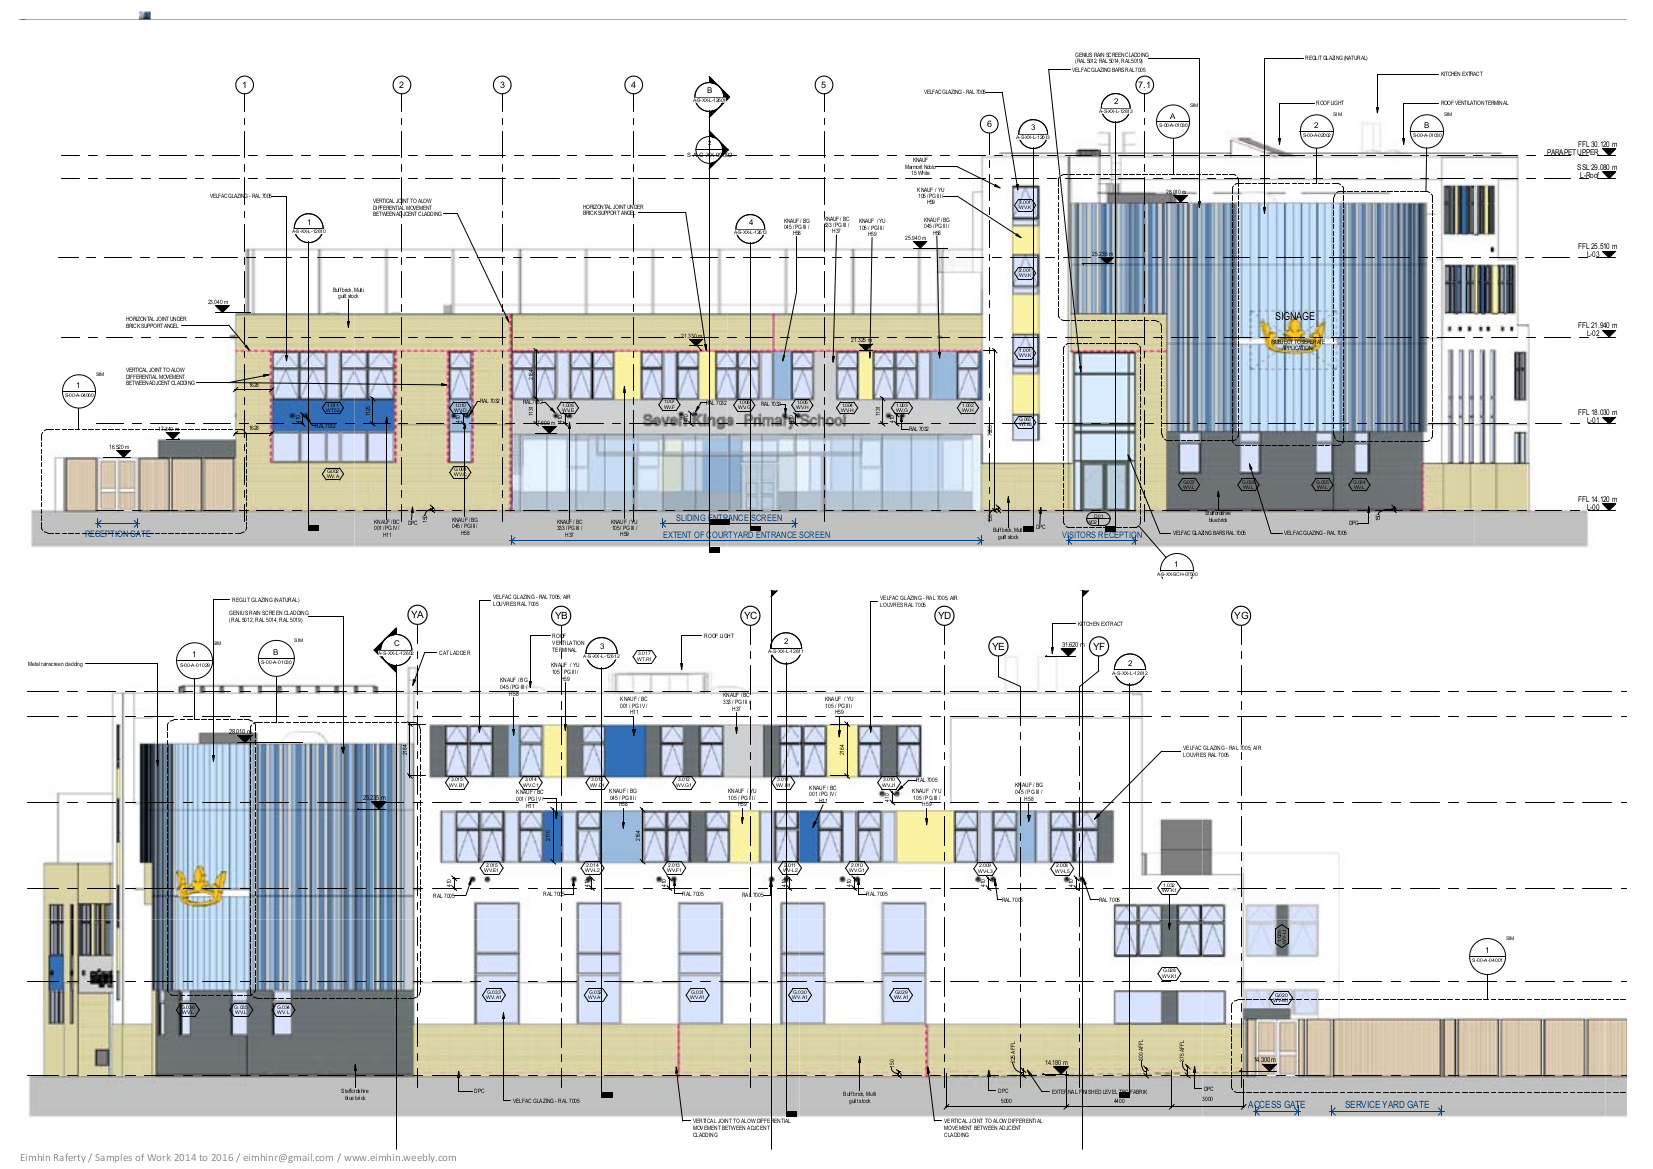
\includegraphics{assets/WGI/WGI-b13.png}

}

\caption{WGI Image}

\end{figure}%%
\begin{figure}[H]

{\centering 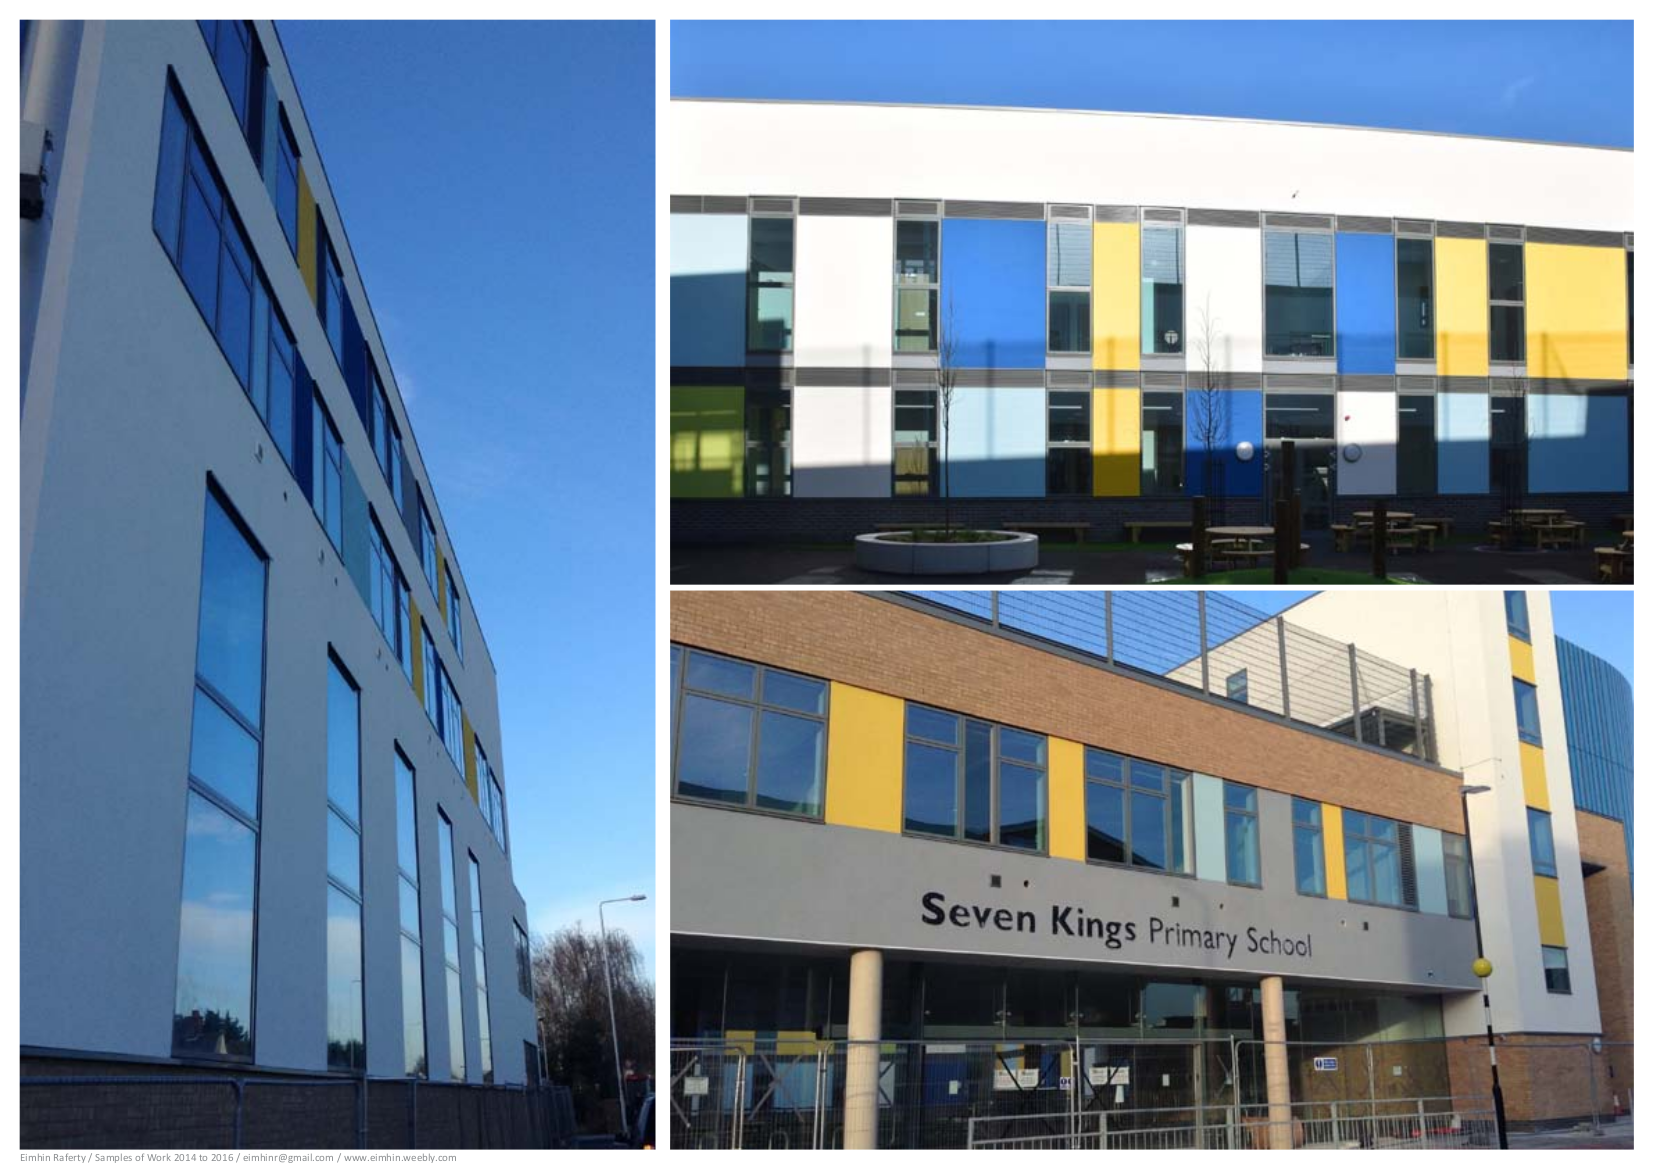
\includegraphics{assets/WGI/WGI-b14.png}

}

\caption{WGI Image}

\end{figure}%%
\begin{figure}[H]

{\centering 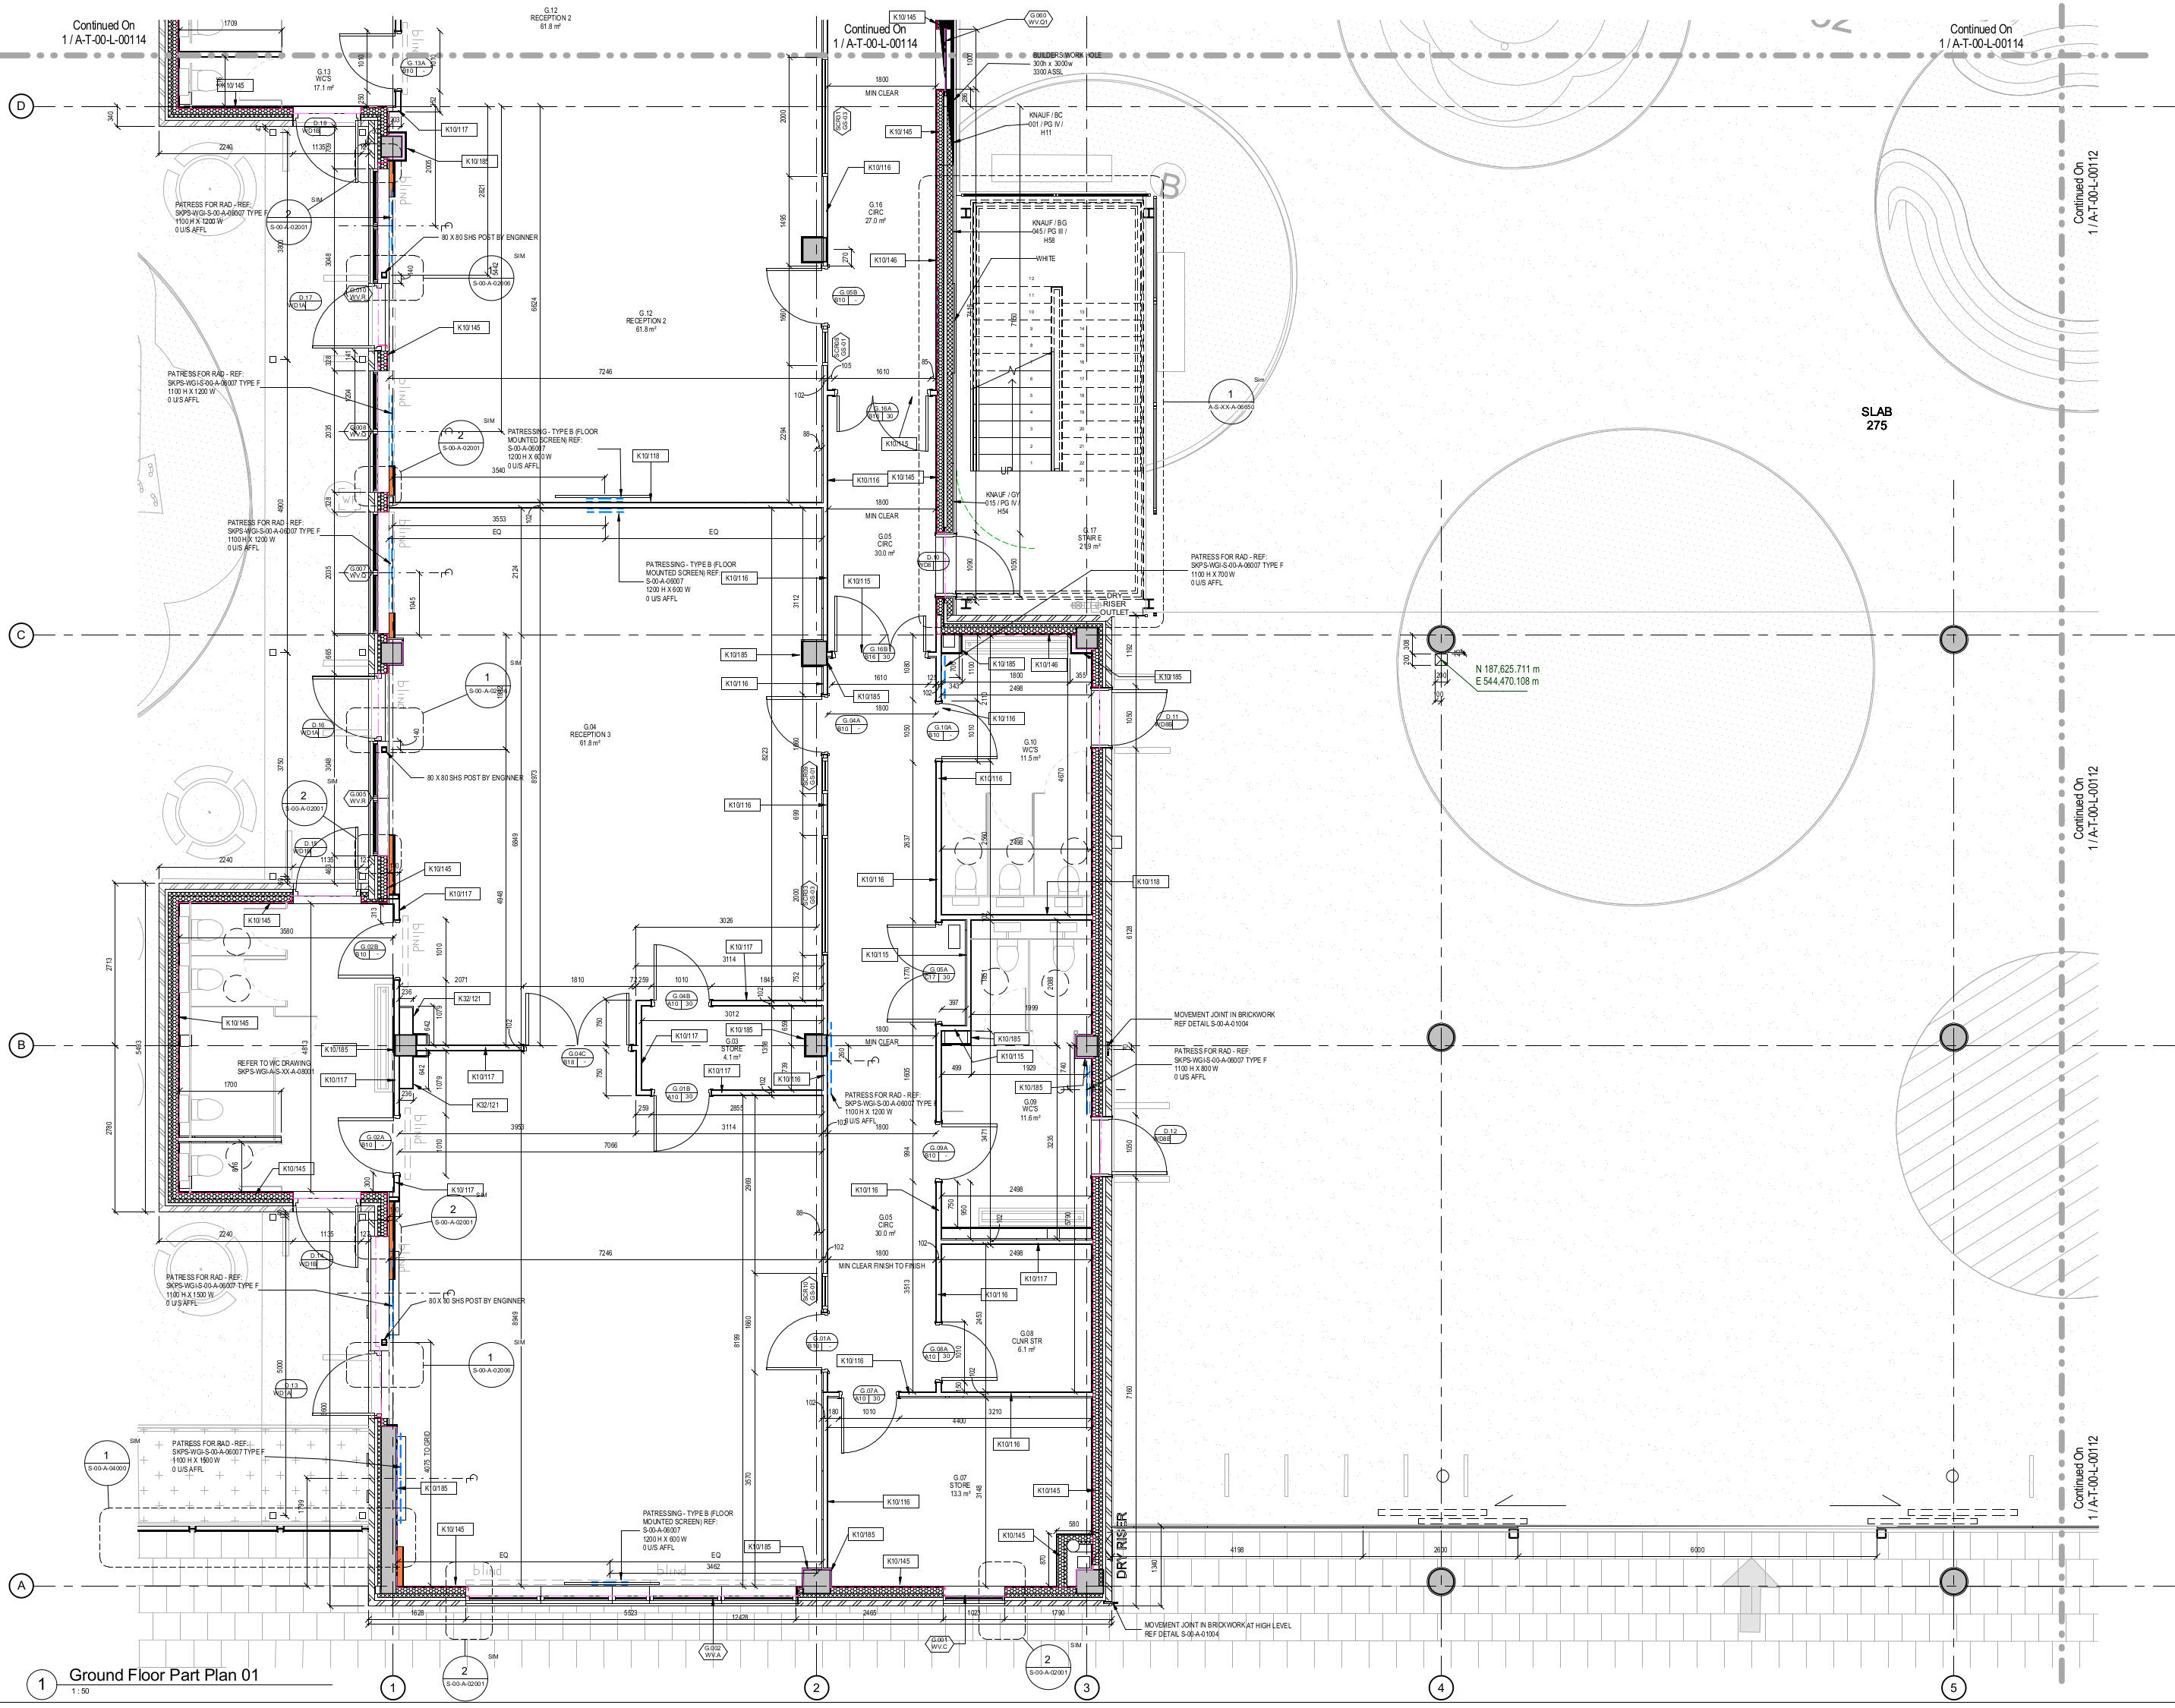
\includegraphics{assets/WGI/WGI-SevenKingsPartPlan.jpg}

}

\caption{WGI Image}

\end{figure}%

\subsubsection{Housing Audits}\label{housing-audits}

\begin{figure}[H]

{\centering 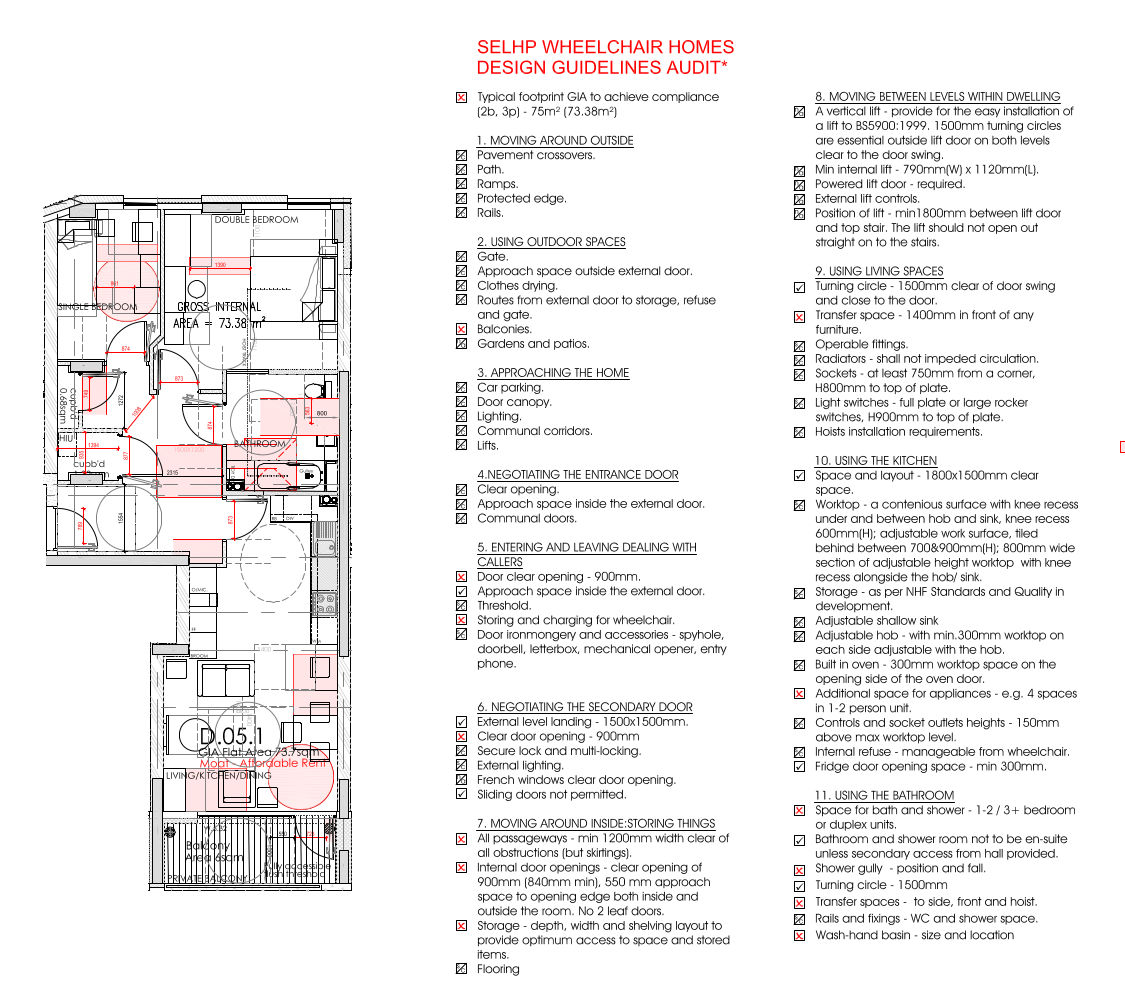
\includegraphics{assets/WGI/WGI-Audit1.jpg}

}

\caption{WGI Image}

\end{figure}%%
\begin{figure}[H]

{\centering 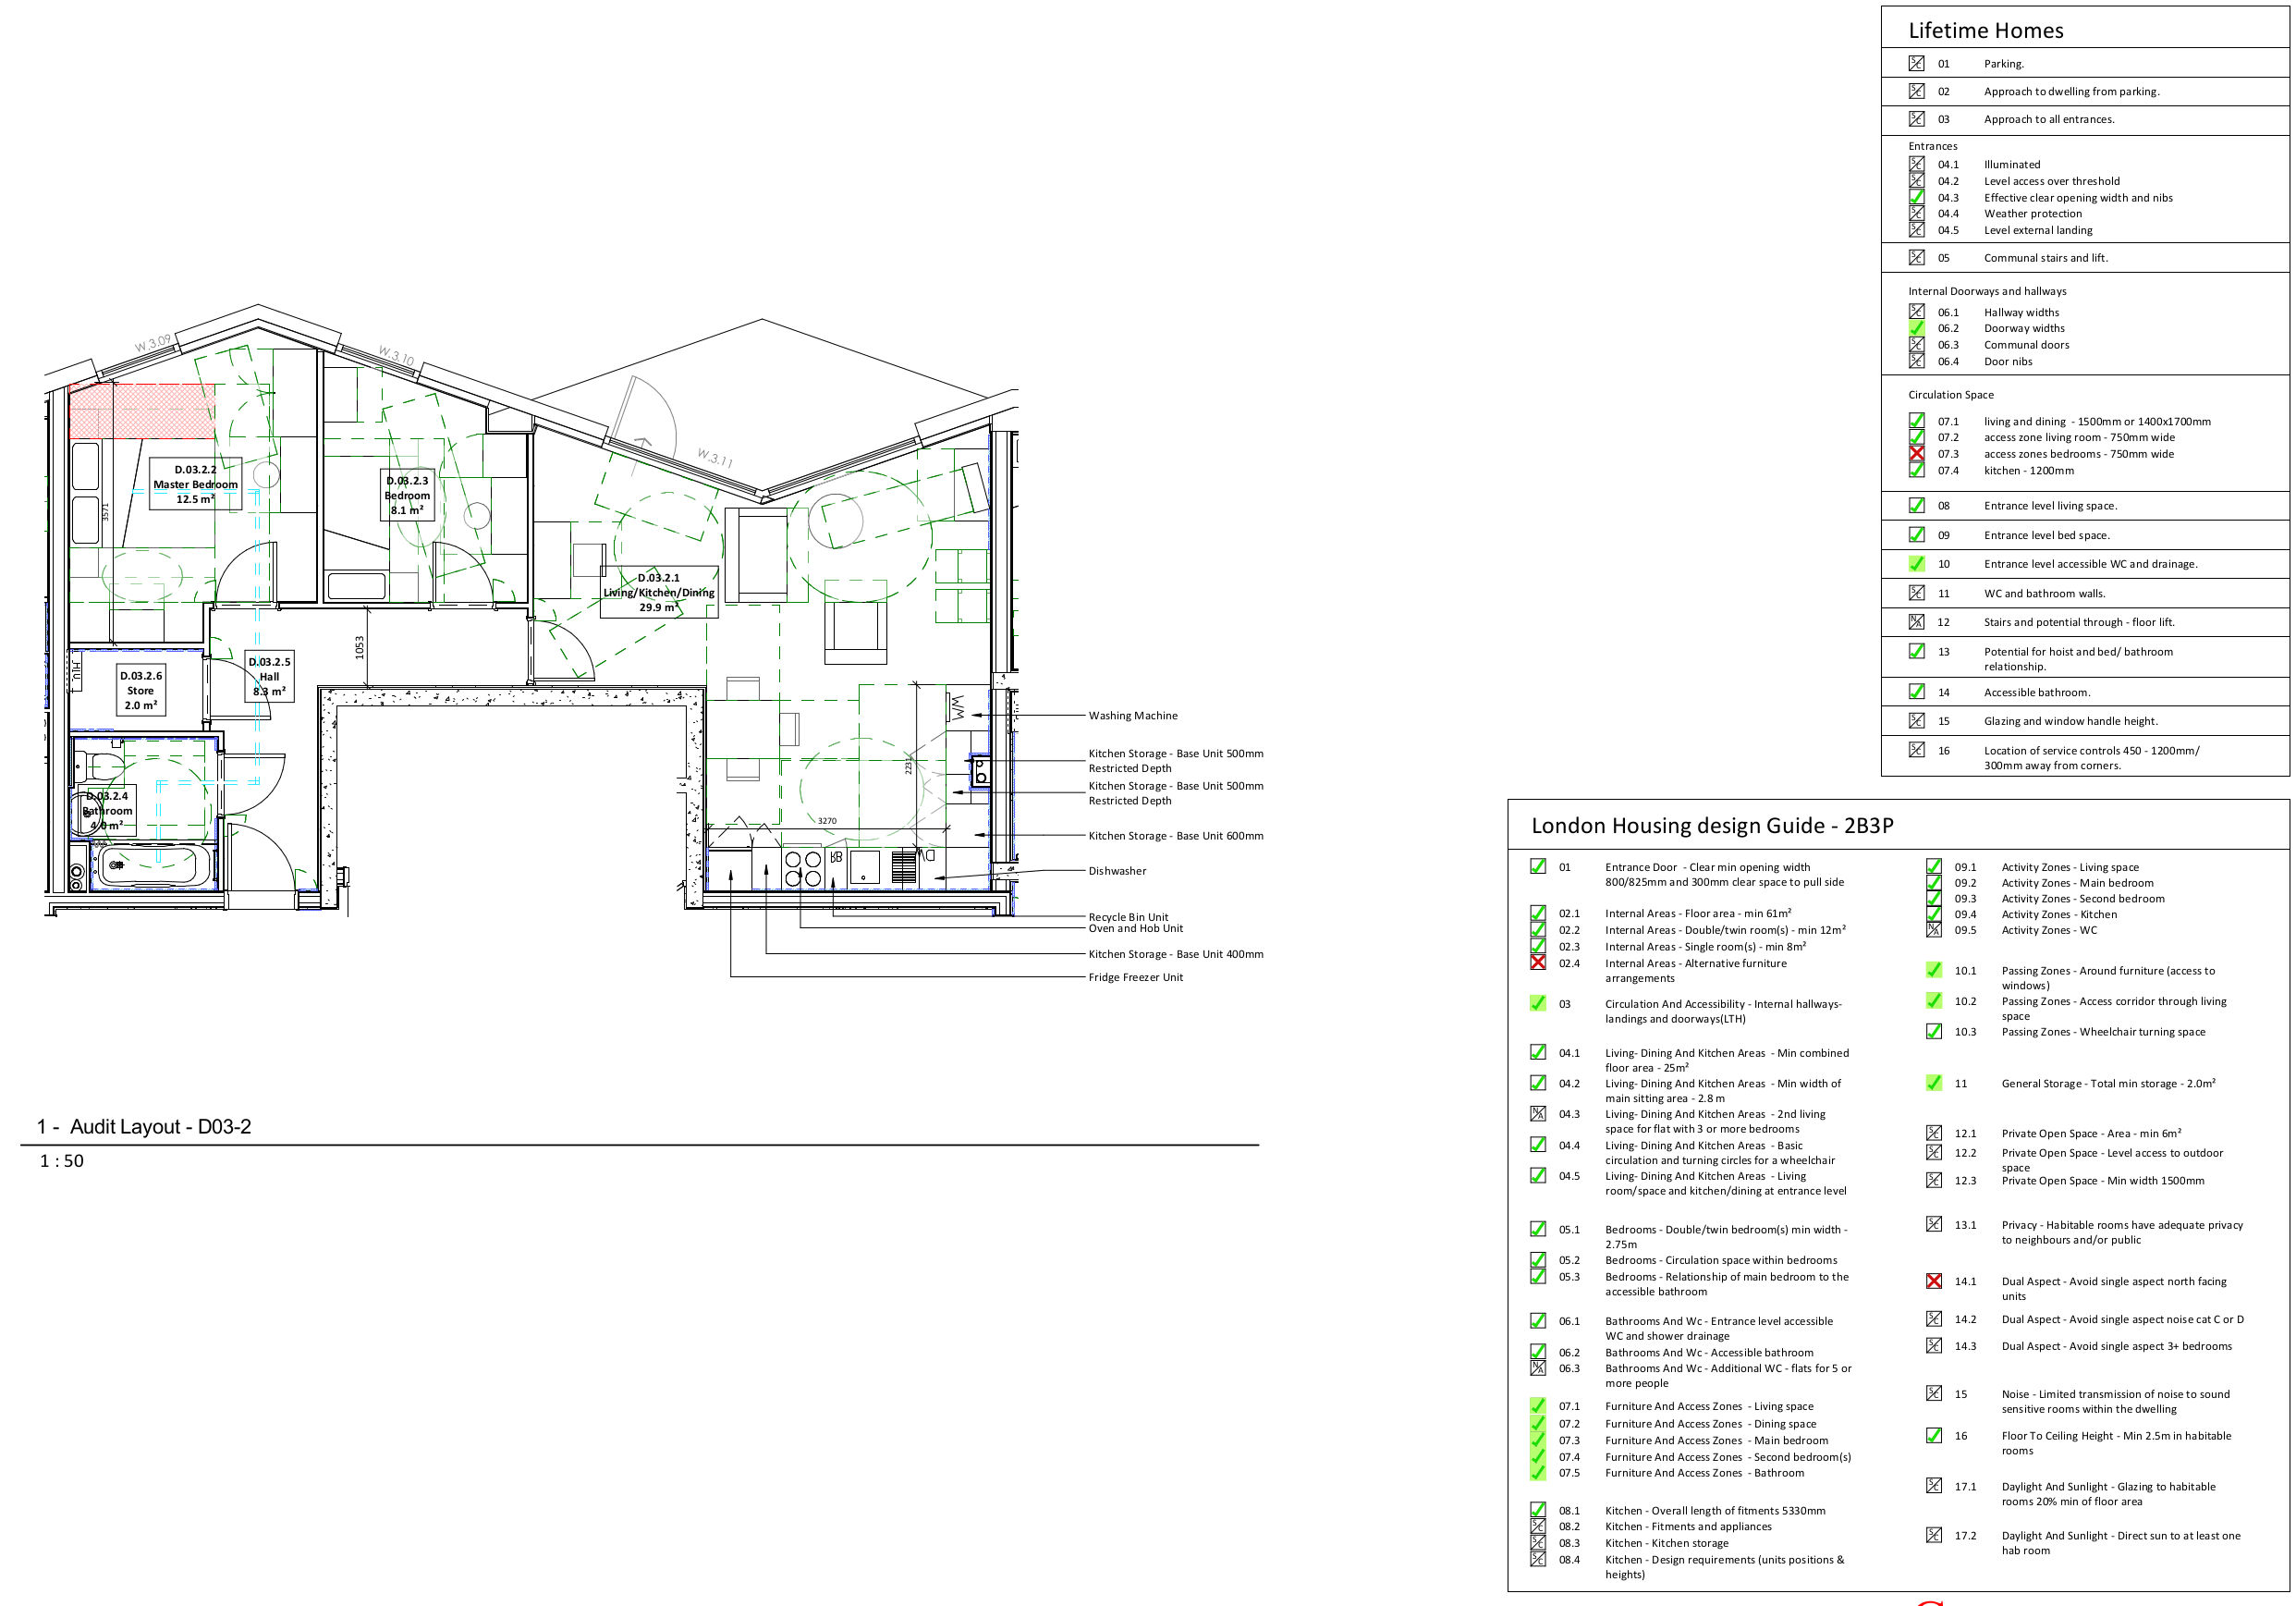
\includegraphics{assets/WGI/WGI-Audit2.jpg}

}

\caption{WGI Image}

\end{figure}%%
\begin{figure}[H]

{\centering 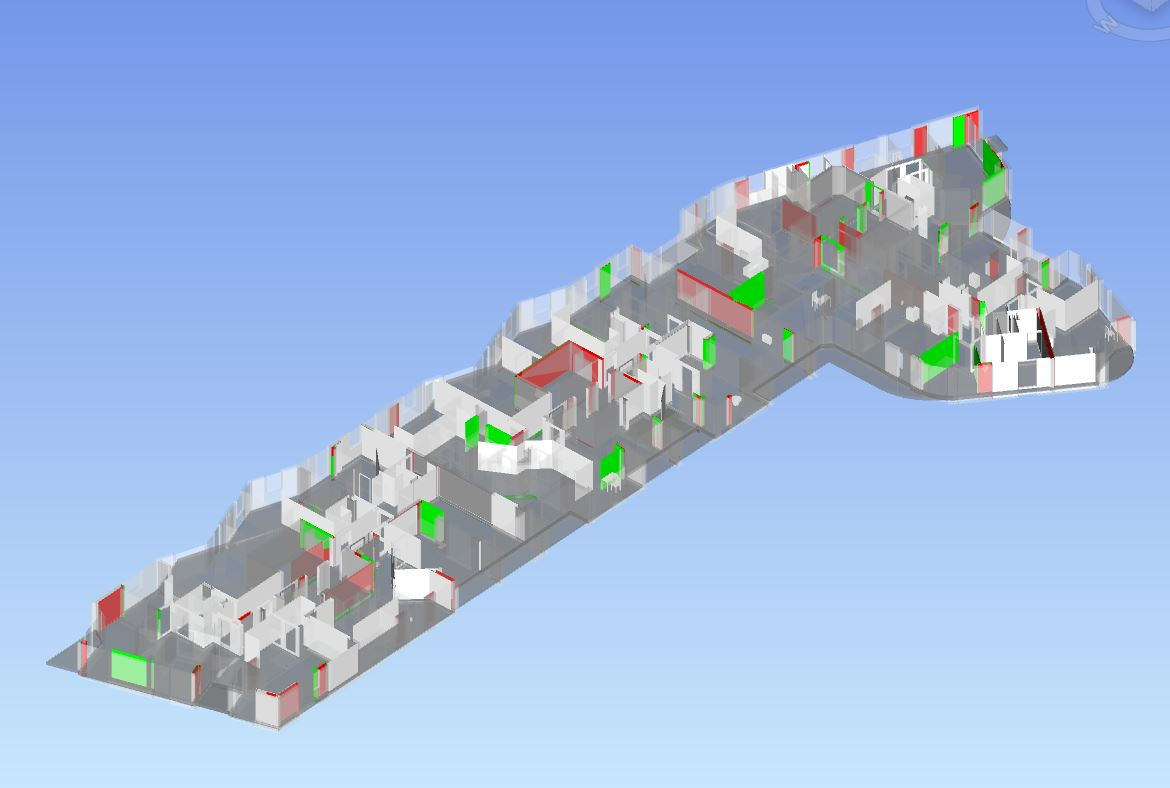
\includegraphics{assets/WGI/WGI-AuditNavis.JPG}

}

\caption{WGI Image}

\end{figure}%%
\begin{figure}[H]

{\centering 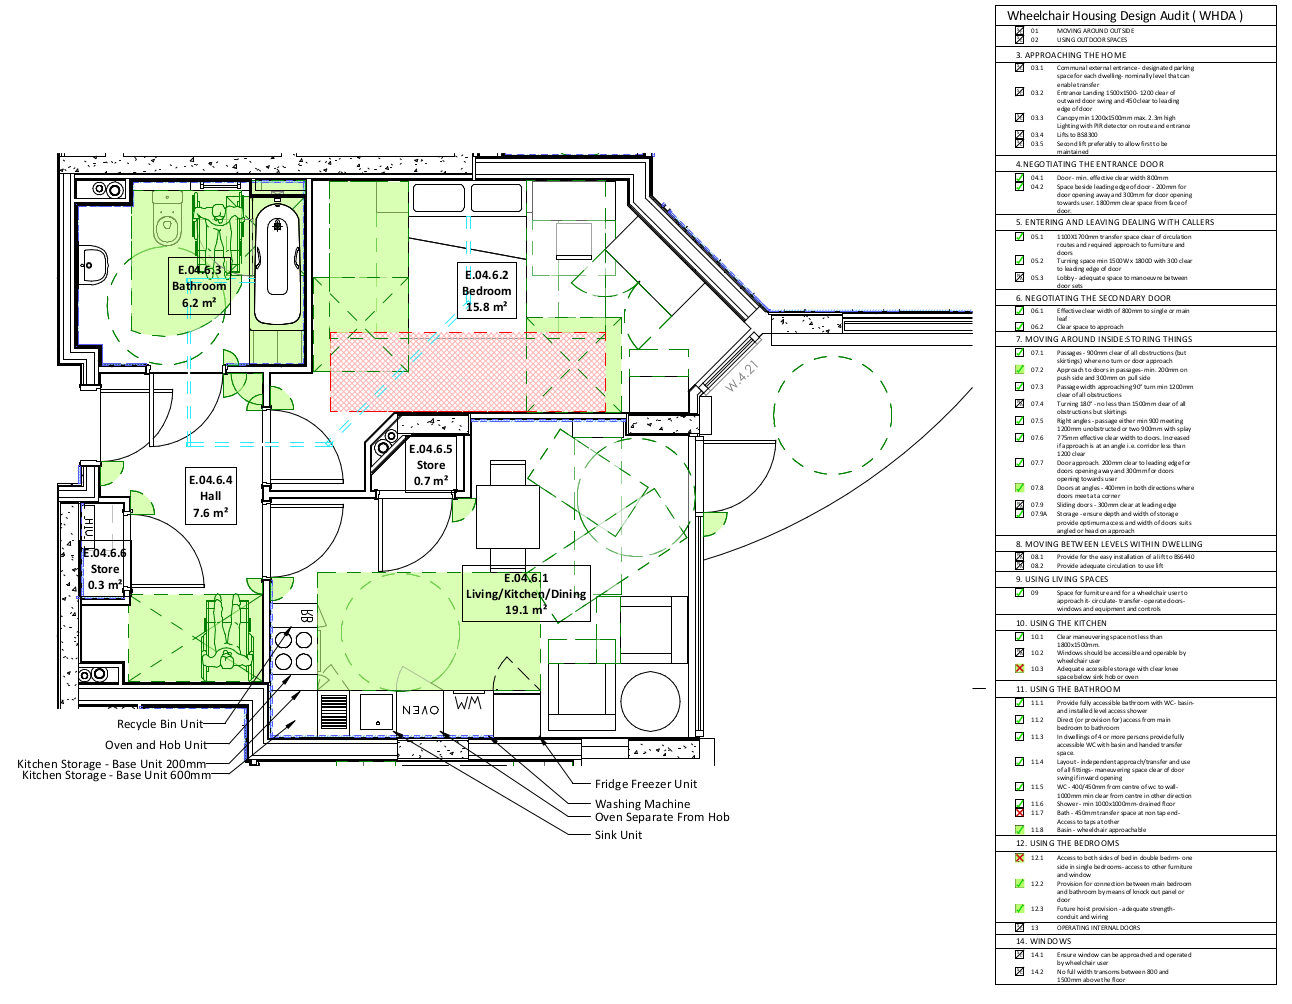
\includegraphics{assets/WGI/WGI-4.png}

}

\caption{WGI Image}

\end{figure}%

\subsubsection{Bromley South Central
Detailing}\label{bromley-south-central-detailing}

\begin{figure}[H]

{\centering 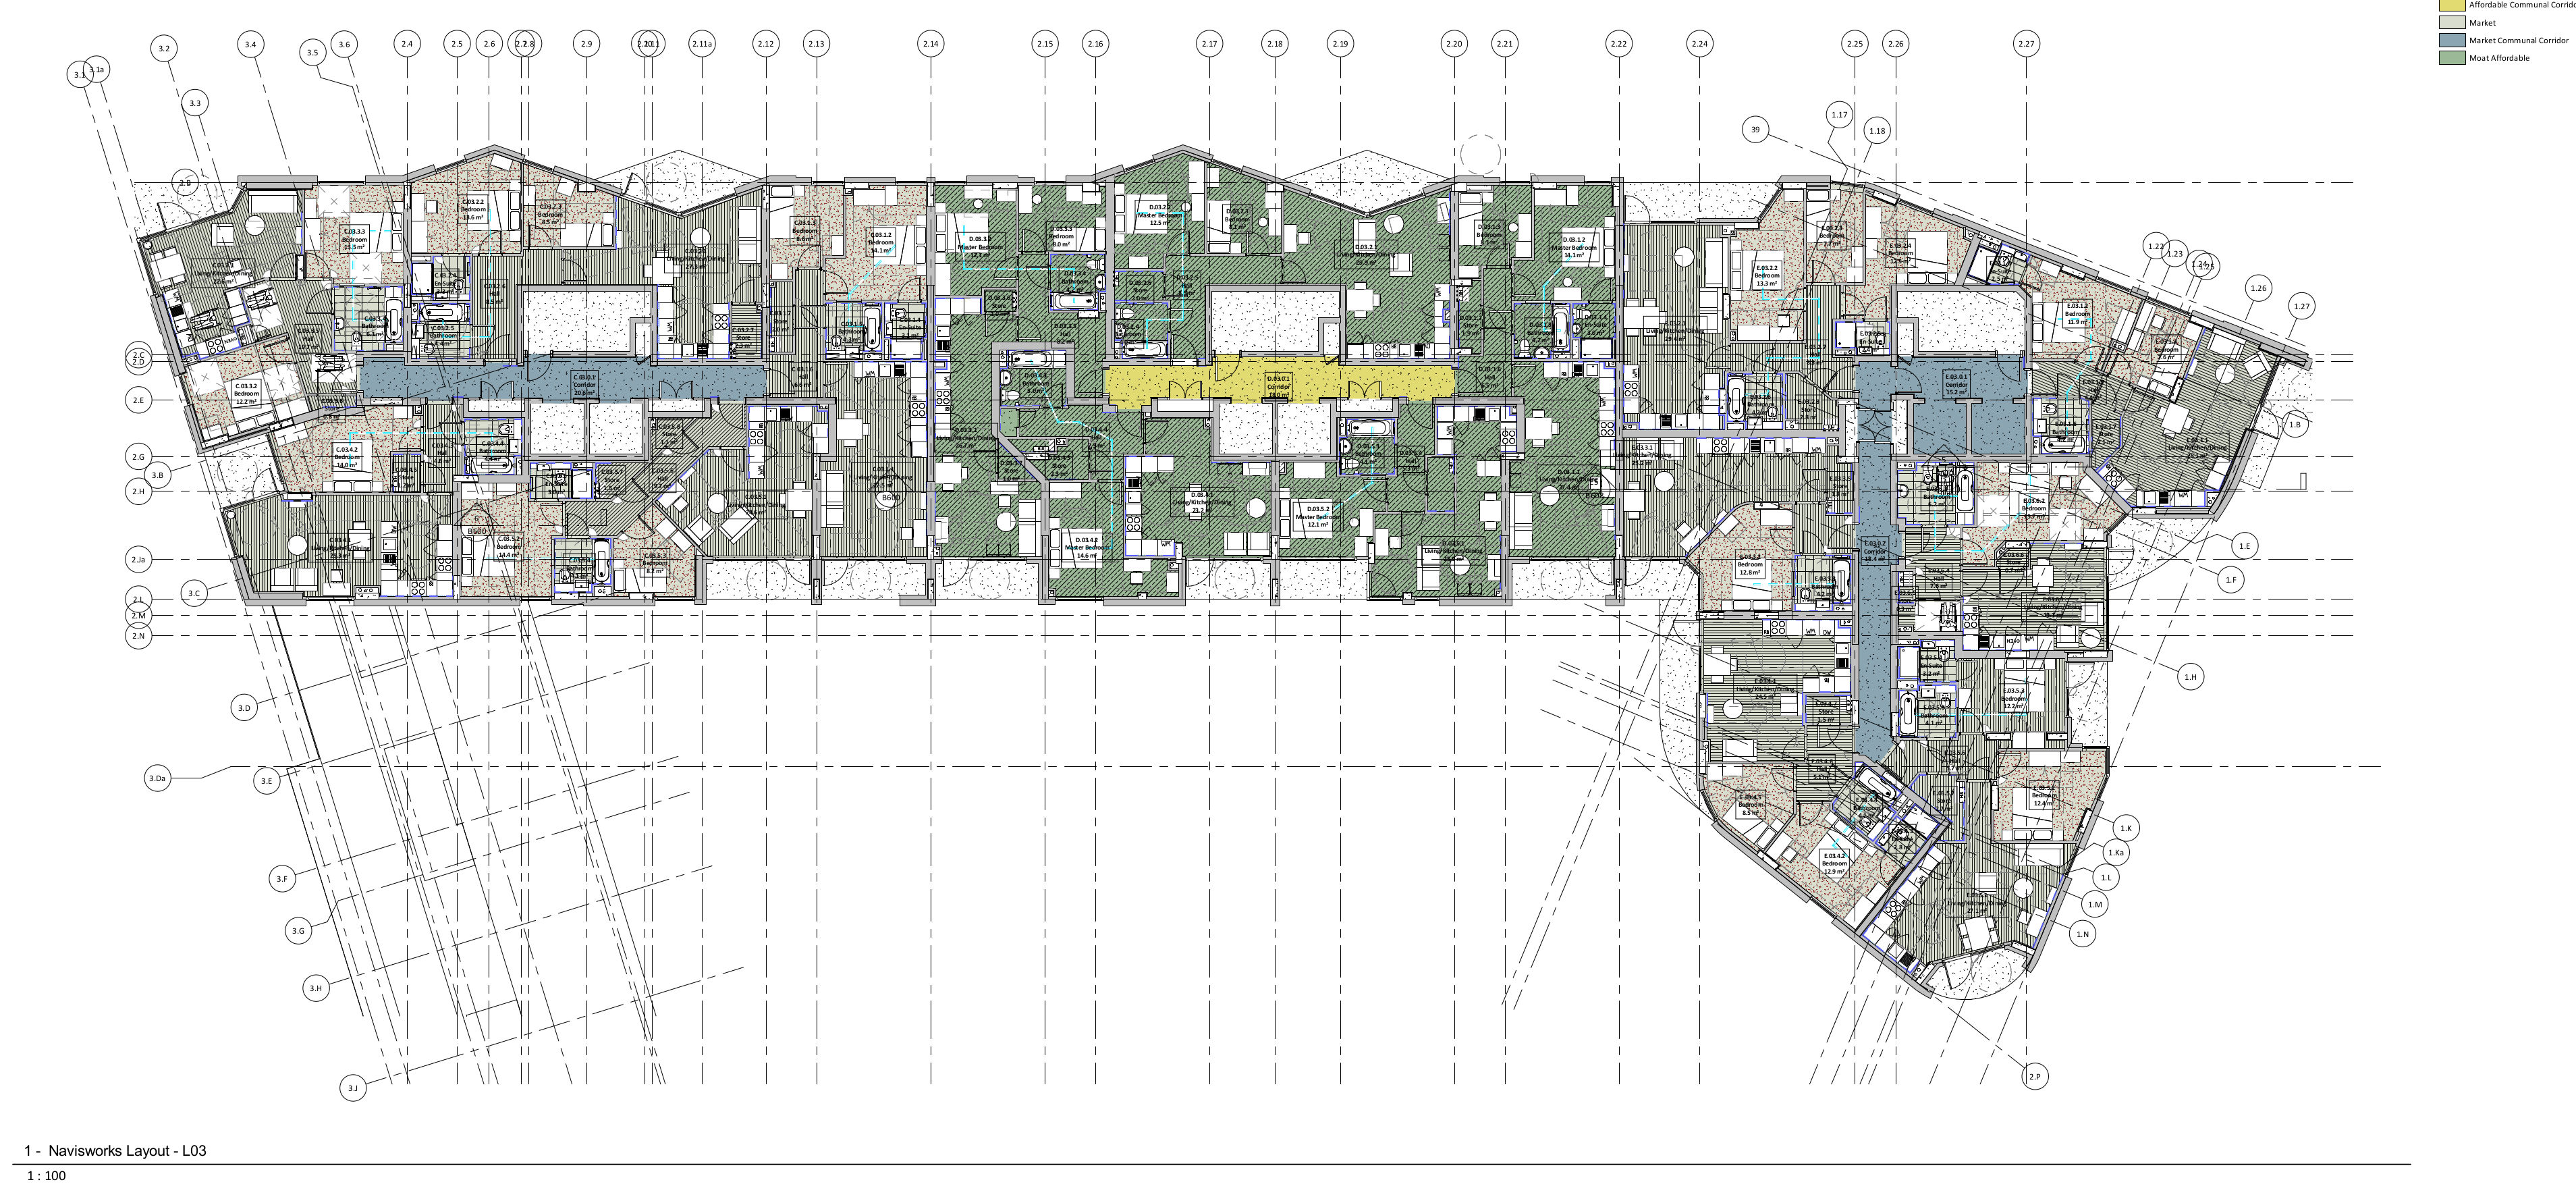
\includegraphics{assets/WGI/WGI-BSC-plan1.jpg}

}

\caption{WGI Image}

\end{figure}%%
\begin{figure}[H]

{\centering 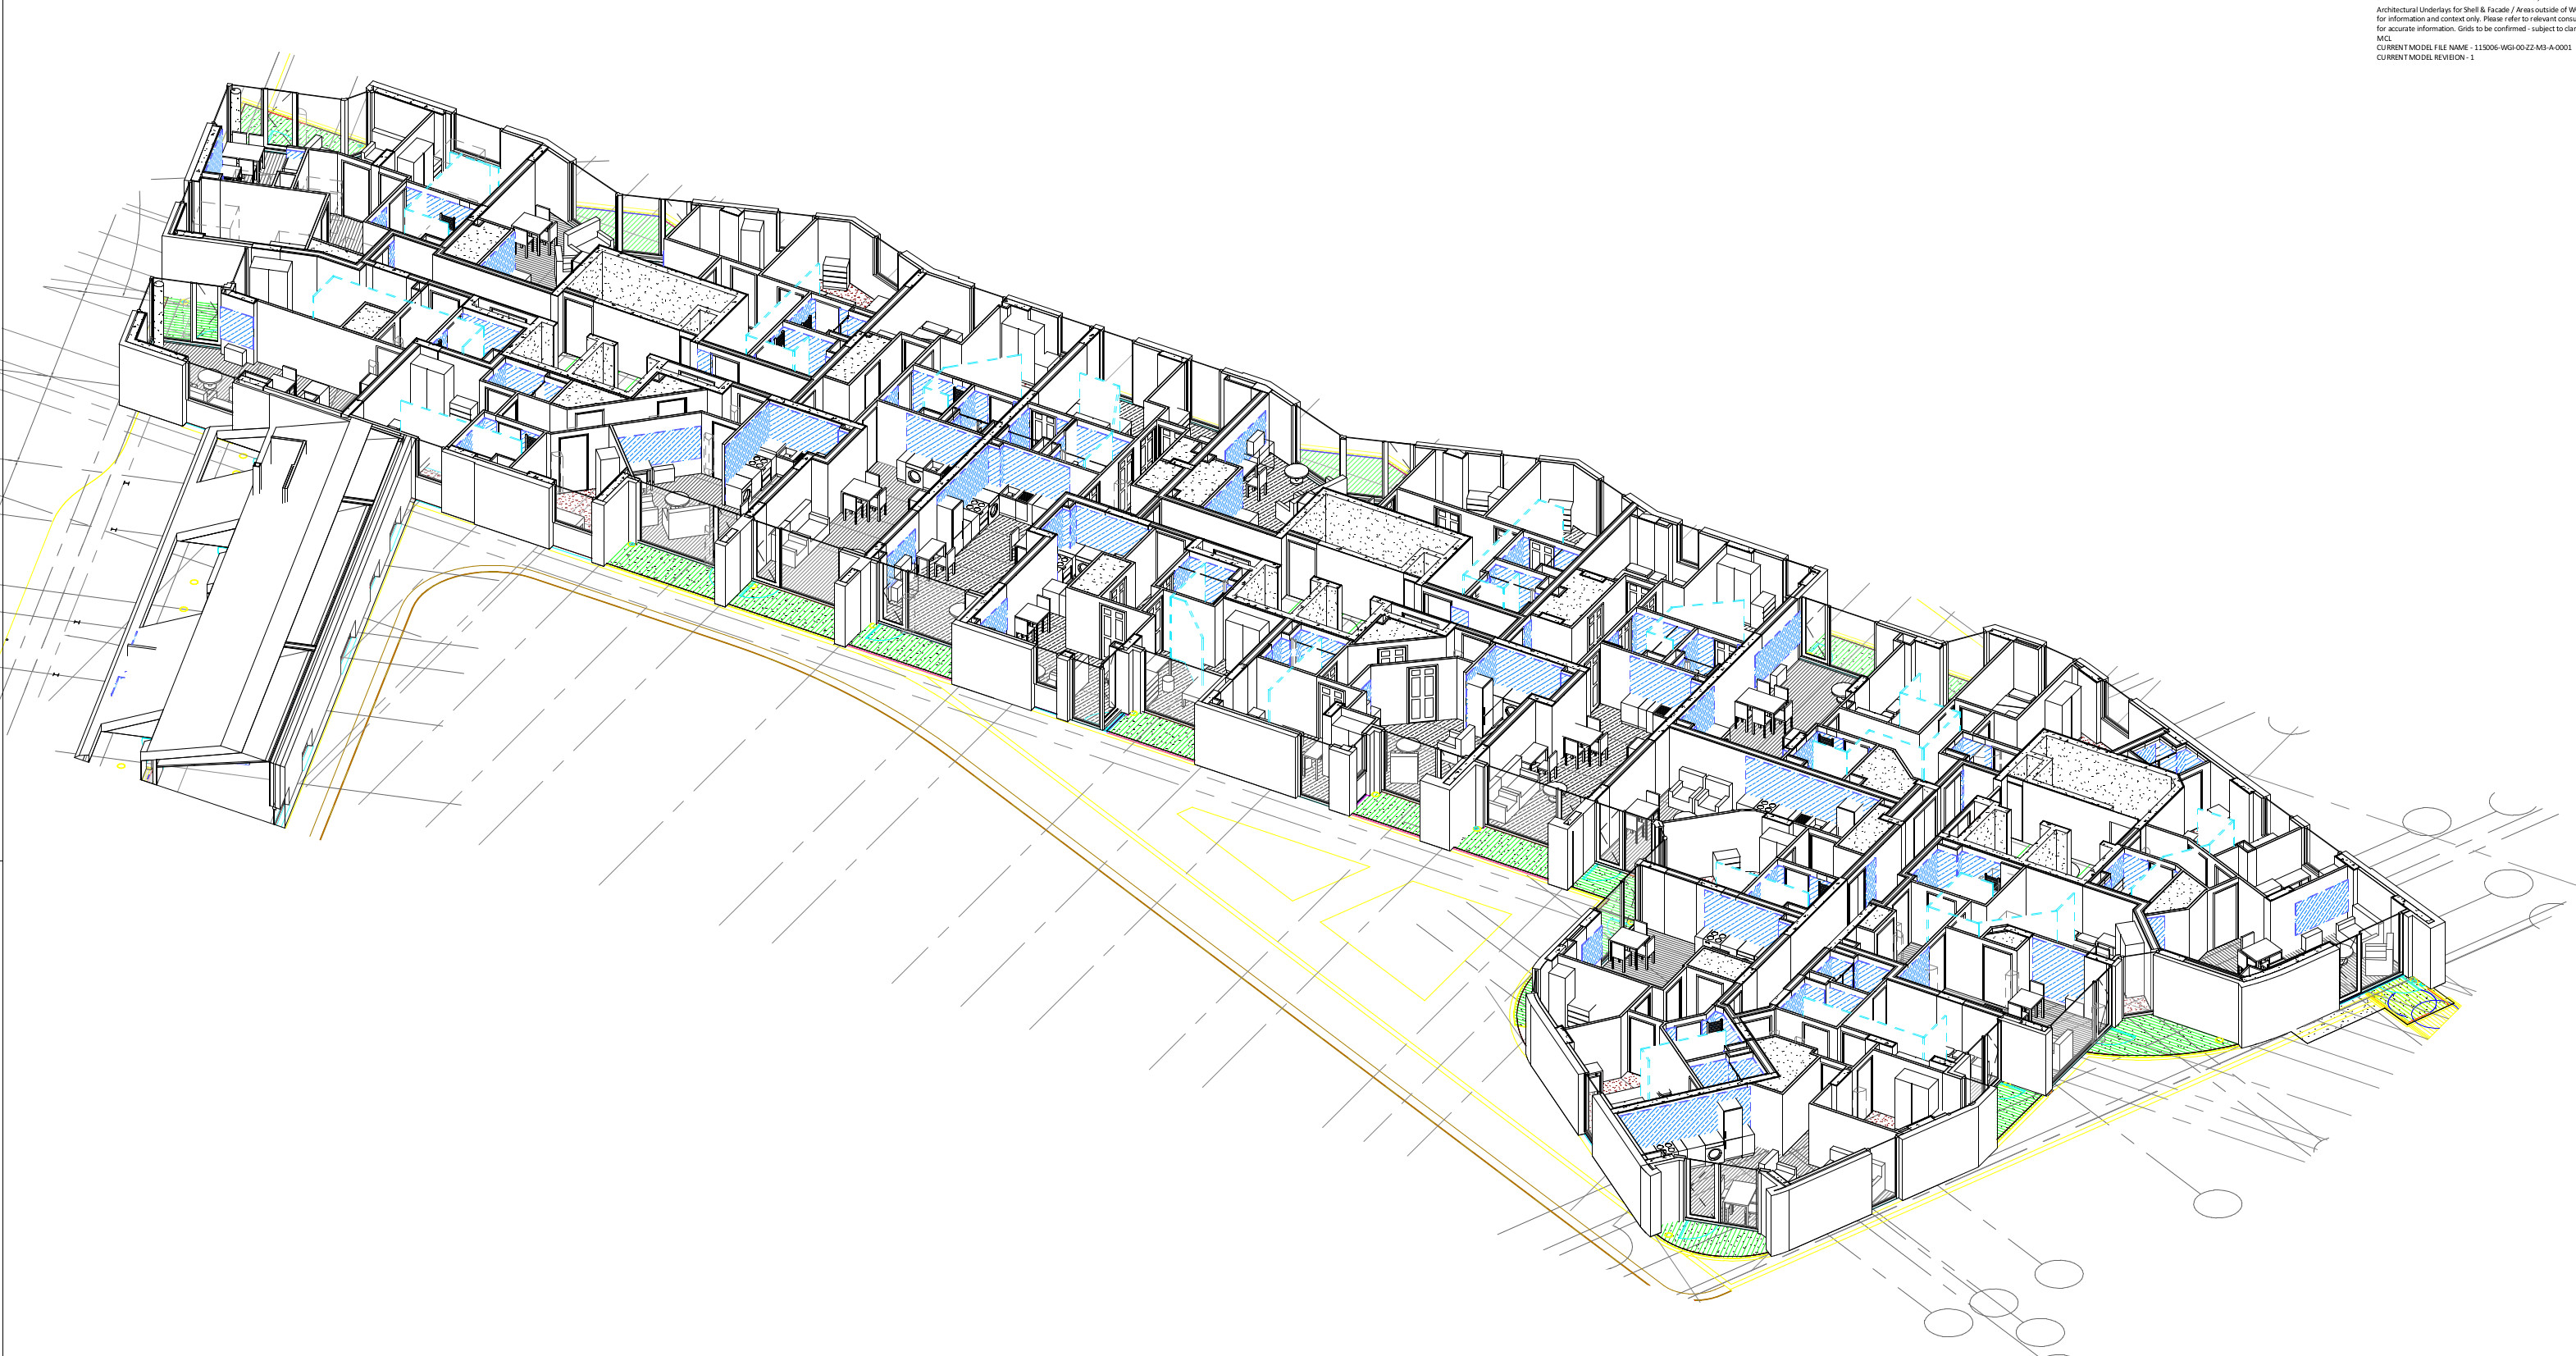
\includegraphics{assets/WGI/WGI-BSC-plan-iso1.jpg}

}

\caption{WGI Image}

\end{figure}%%
\begin{figure}[H]

{\centering 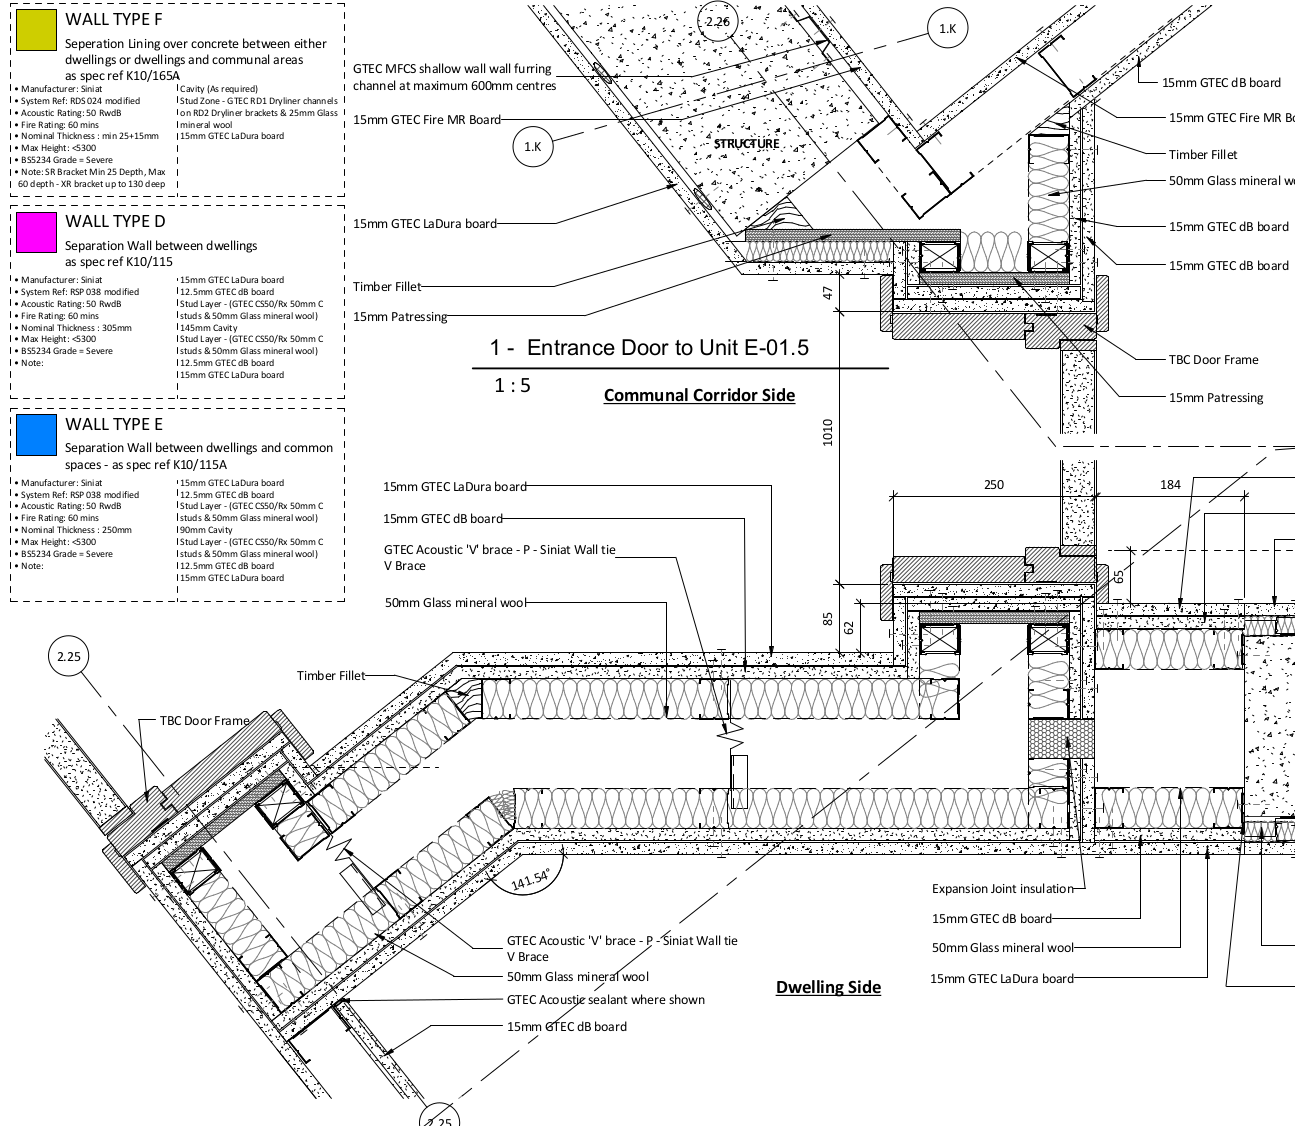
\includegraphics{assets/WGI/WGI-6.png}

}

\caption{WGI Image}

\end{figure}%%
\begin{figure}[H]

{\centering 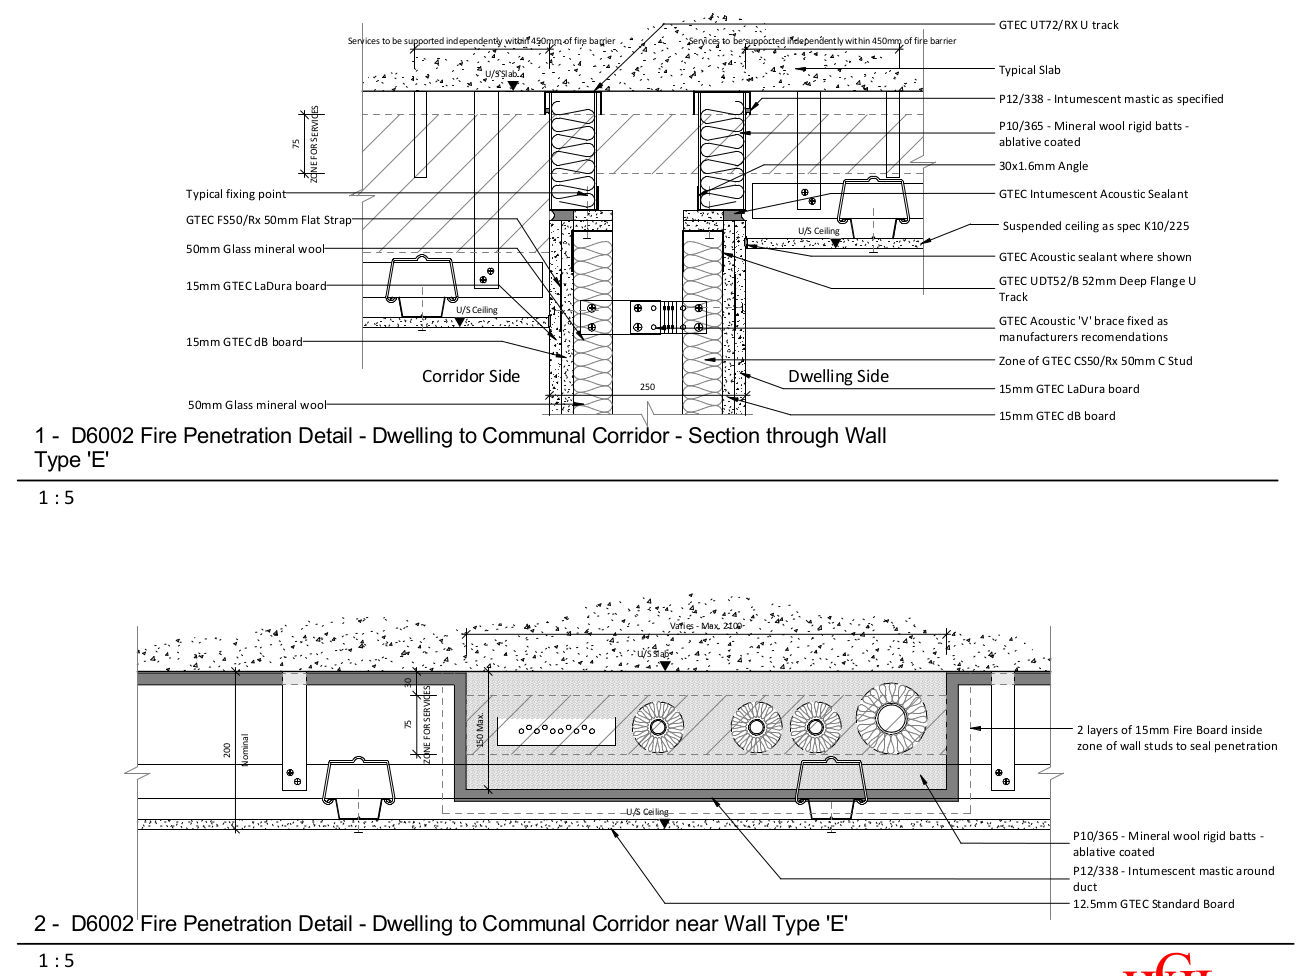
\includegraphics{assets/WGI/WGI-BSC-details2.jpg}

}

\caption{WGI Image}

\end{figure}%%
\begin{figure}[H]

{\centering 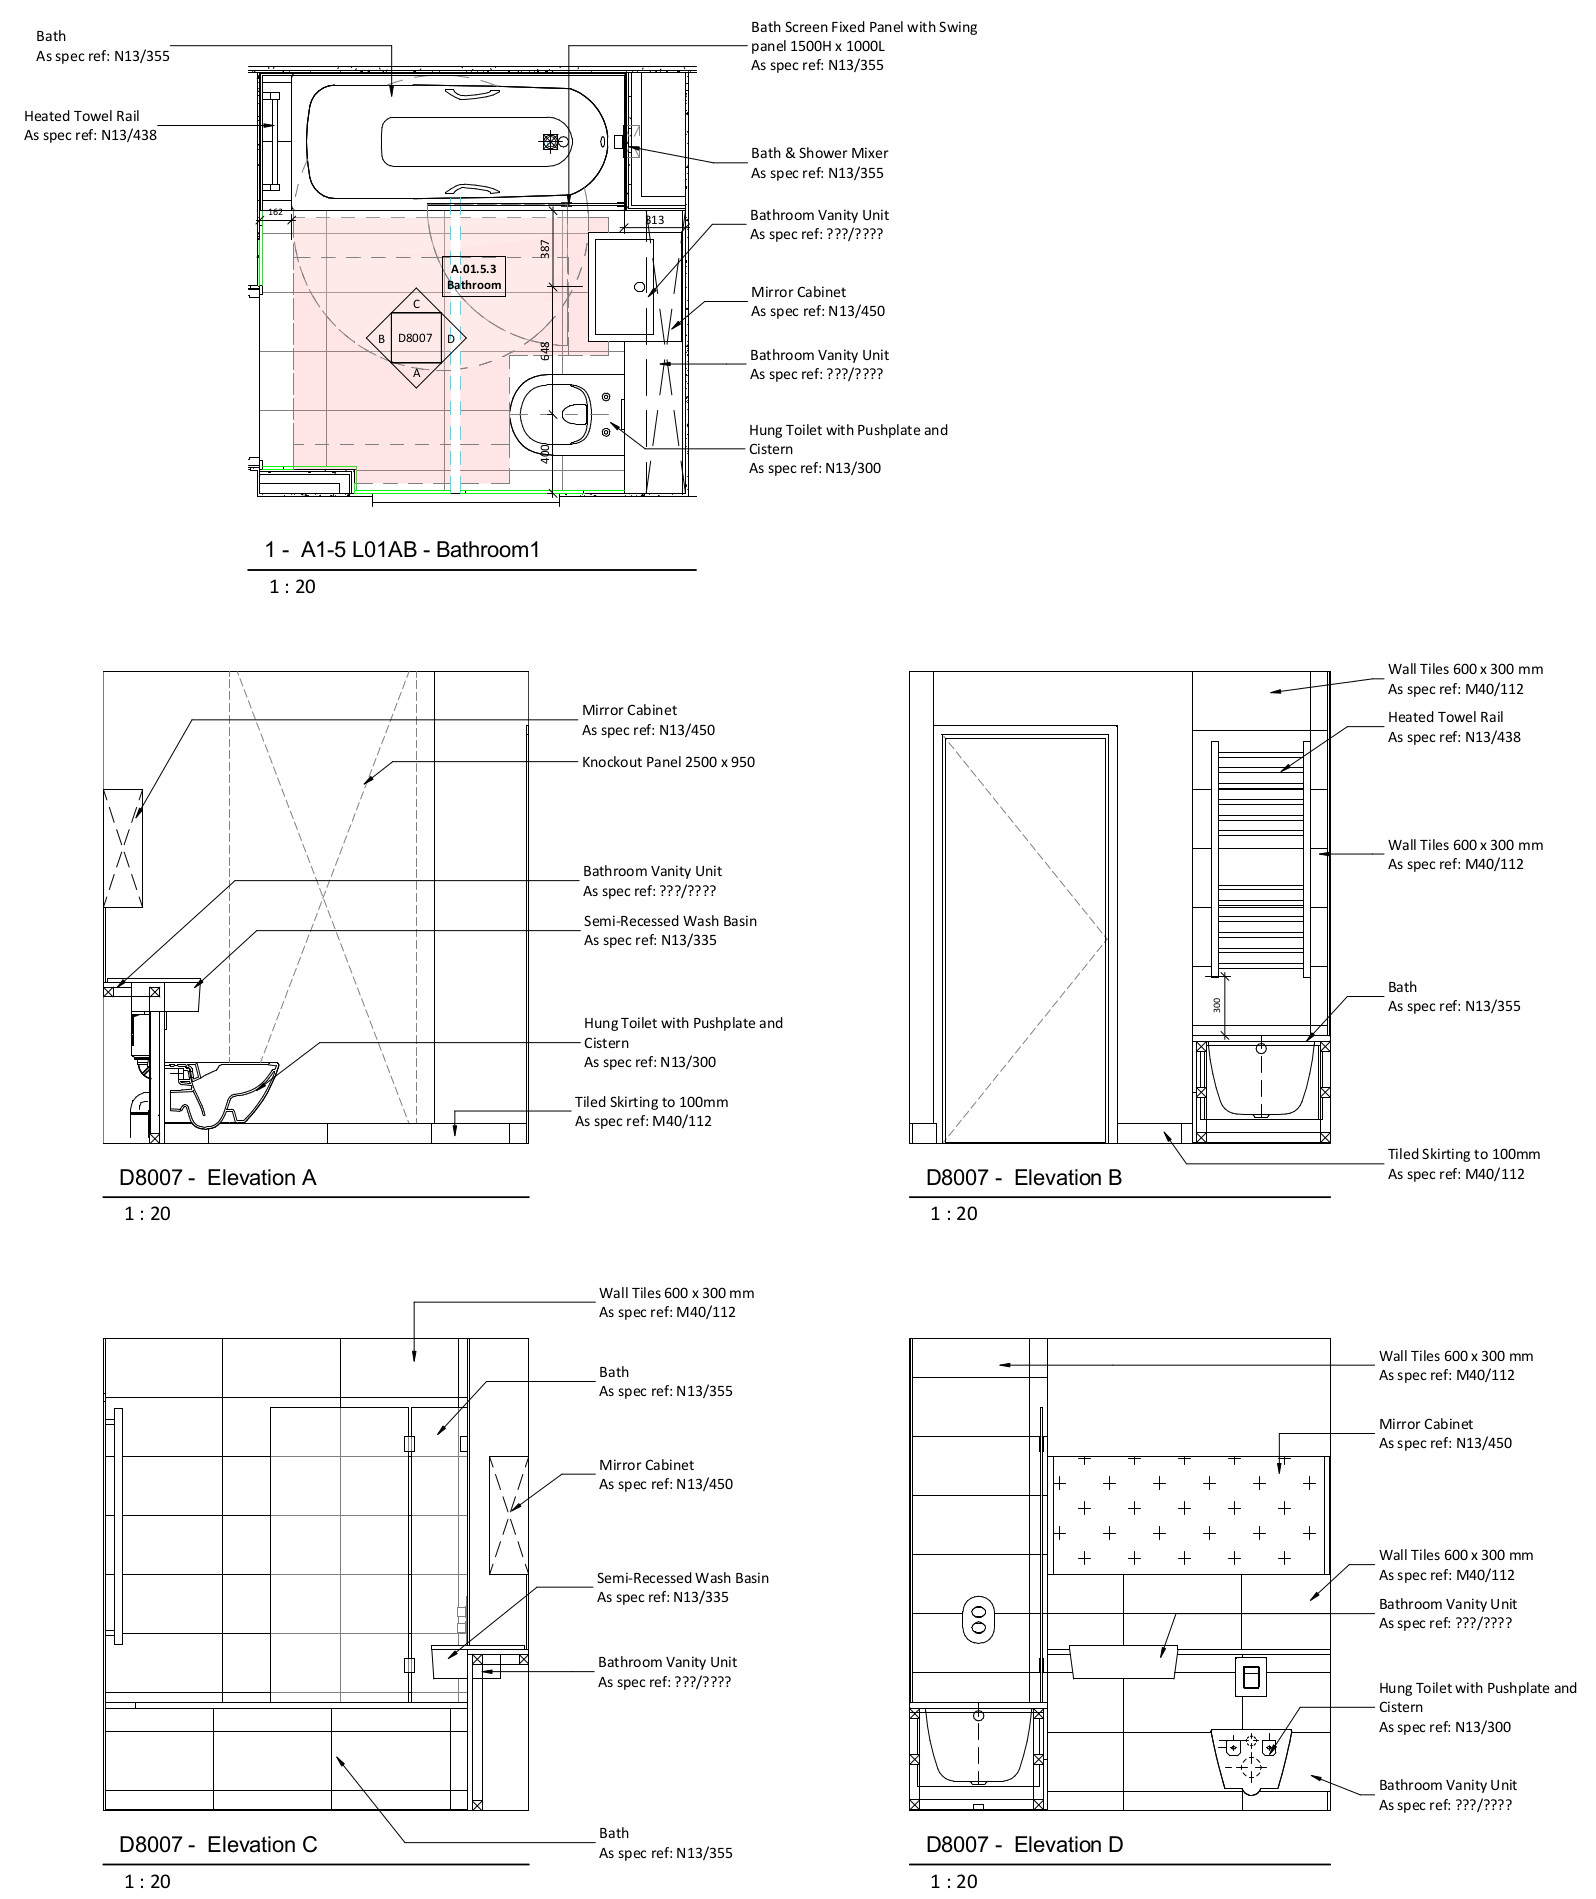
\includegraphics{assets/WGI/WGI-BSC-Detail1.jpg}

}

\caption{WGI Image}

\end{figure}%%
\begin{figure}[H]

{\centering 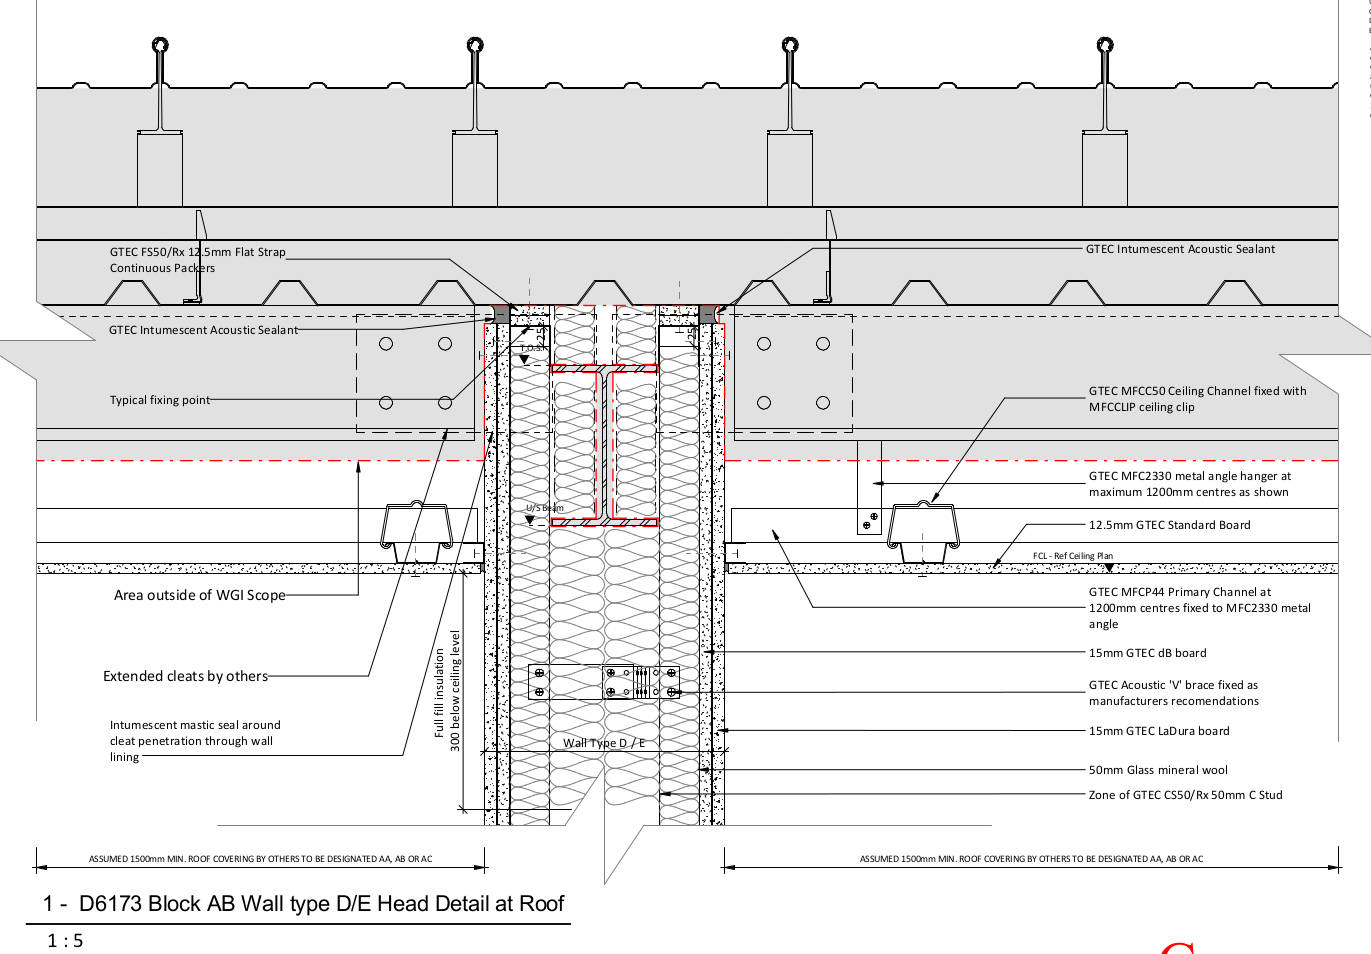
\includegraphics{assets/WGI/WGI-RoofDetail.jpg}

}

\caption{WGI Image}

\end{figure}%

\subsubsection{GOSH Int. Private Patients
Wing}\label{gosh-int.-private-patients-wing}

\begin{figure}[H]

{\centering \includegraphics{assets/WGI/WGI-IPP-SitePhoto.JPG}

}

\caption{WGI Image}

\end{figure}%%
\begin{figure}[H]

{\centering \includegraphics{assets/WGI/WGI-IPP-002.jpg}

}

\caption{WGI Image}

\end{figure}%%
\begin{figure}[H]

{\centering 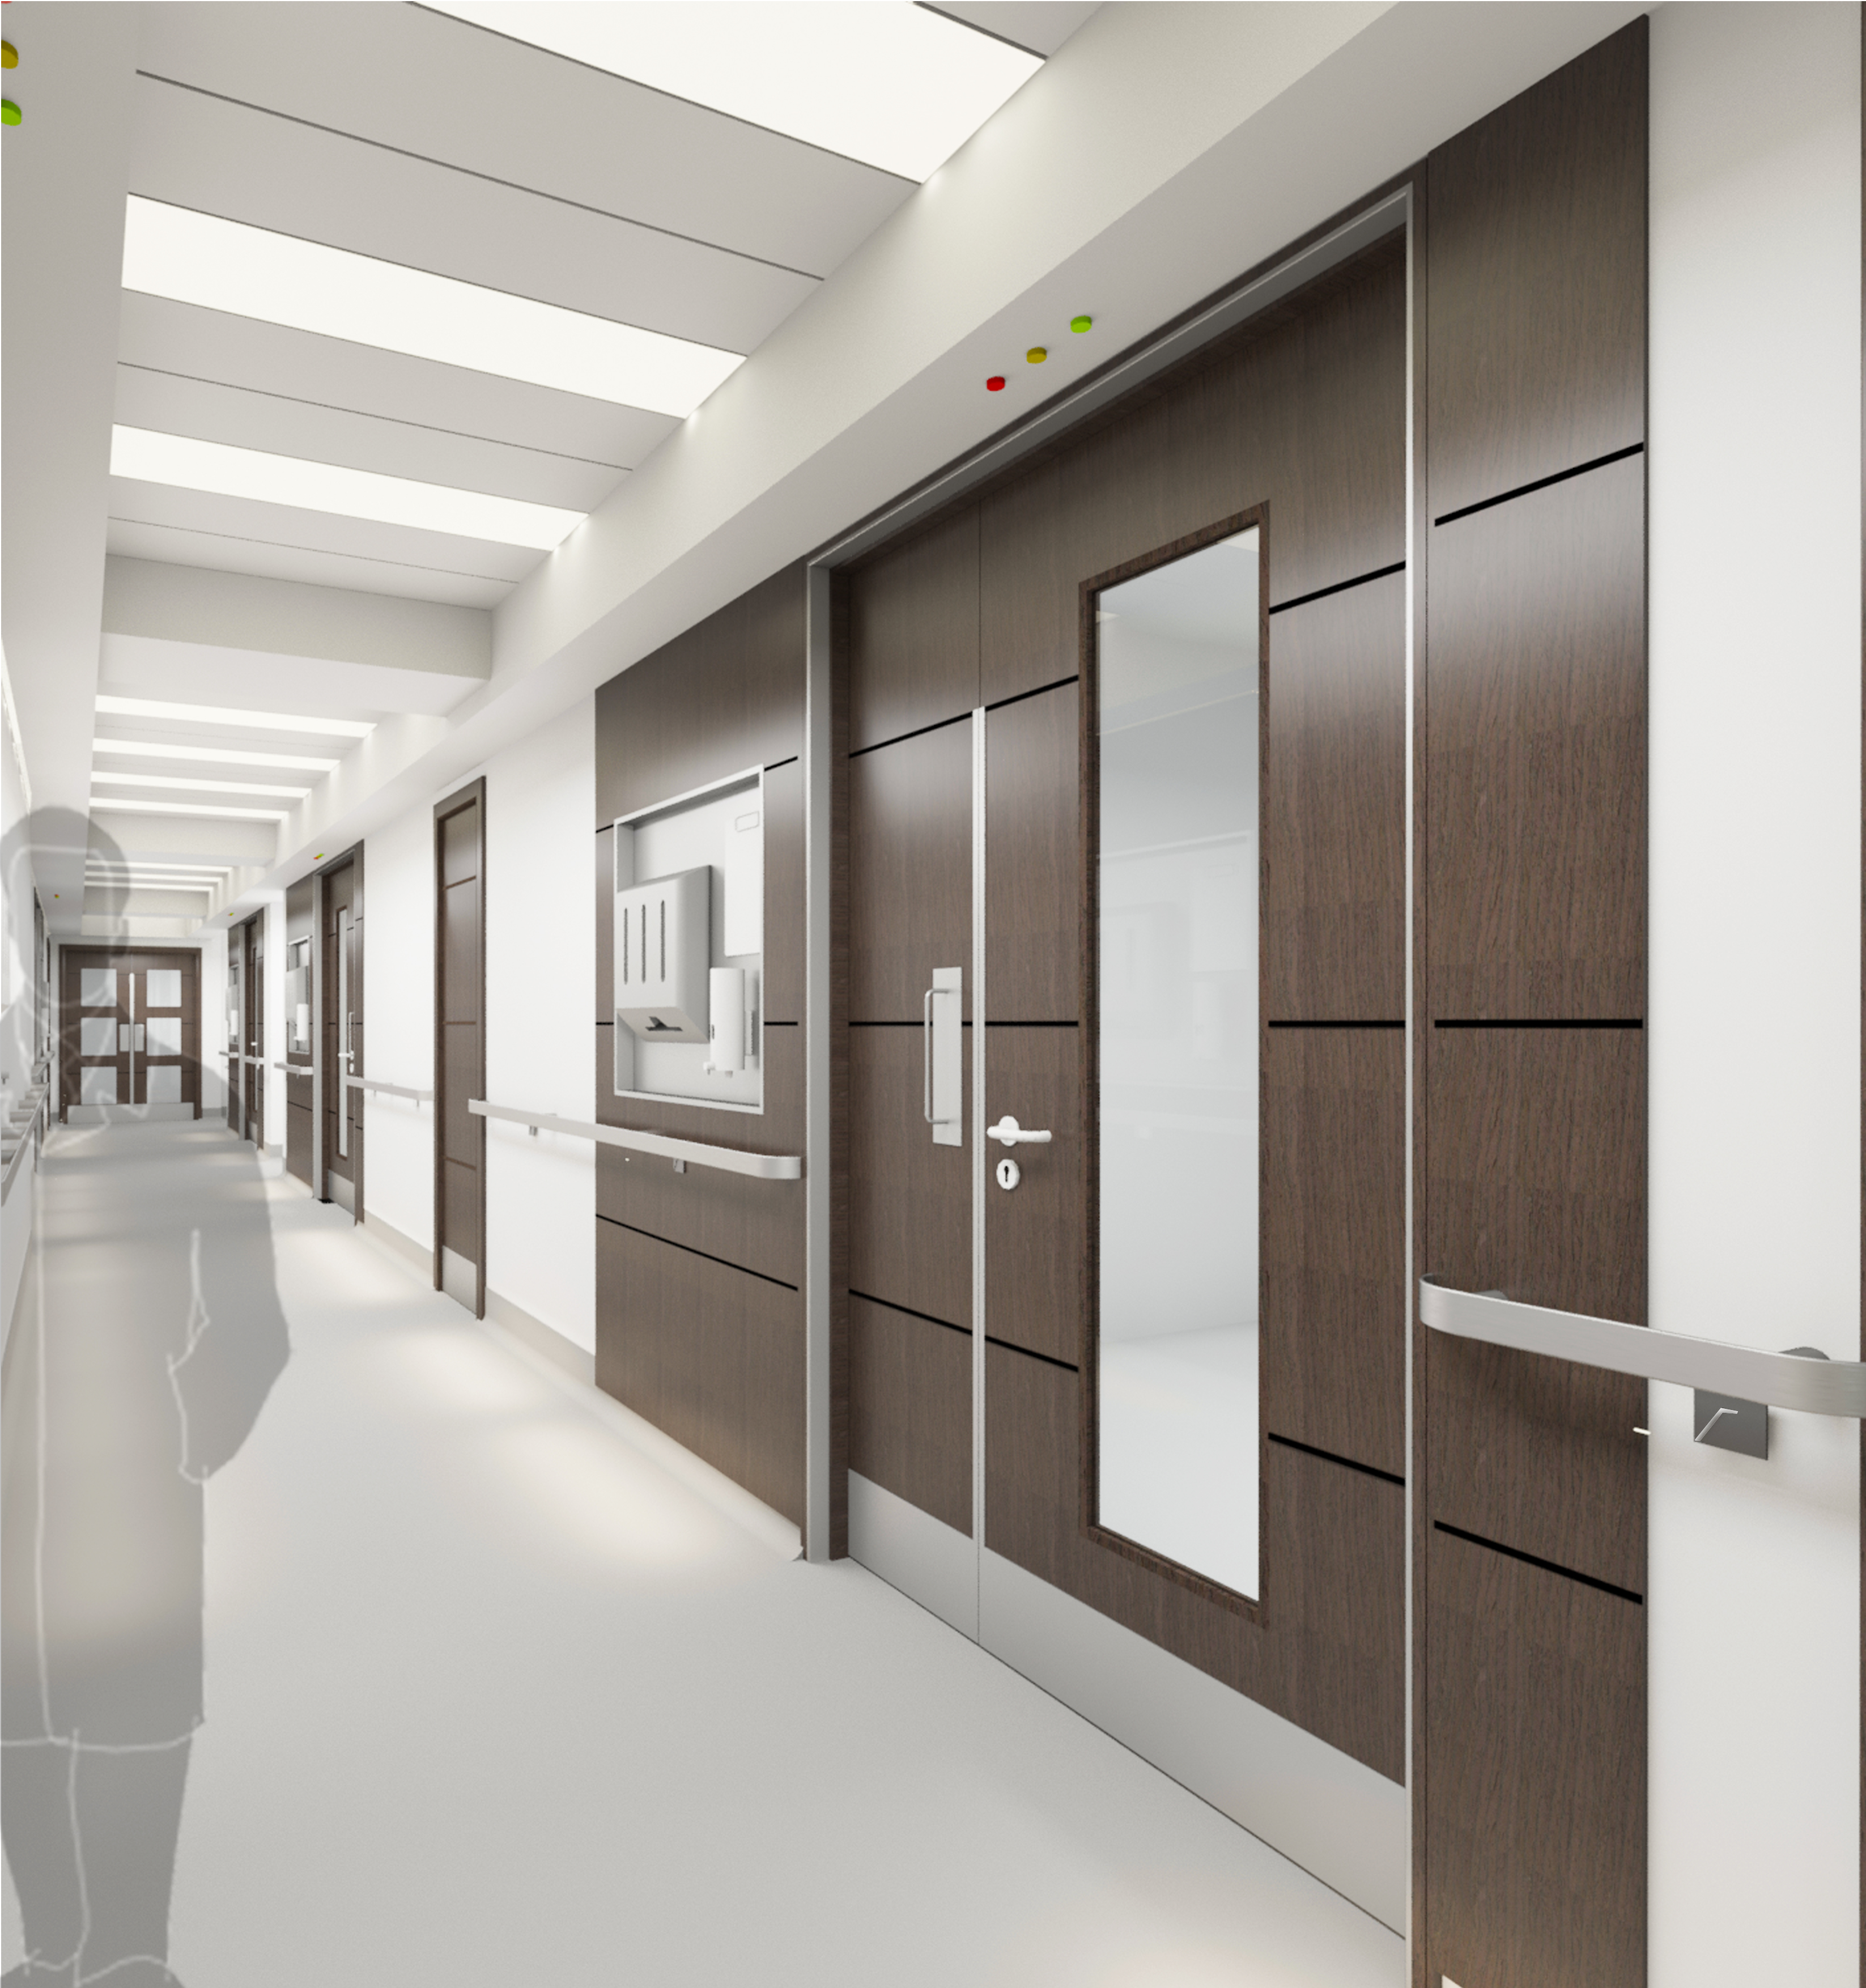
\includegraphics{assets/WGI/WGI-IPP-006.jpg}

}

\caption{WGI Image}

\end{figure}%

\subsubsection{Other Projects}\label{other-projects}

\paragraph{Office Rapid Prototype,
Leeds}\label{office-rapid-prototype-leeds}

\begin{figure}[H]

{\centering \includegraphics{assets/WGI/WGI-2.png}

}

\caption{WGI Image}

\end{figure}%

\paragraph{Residential units in tower and bar building,
London}\label{residential-units-in-tower-and-bar-building-london}

\begin{figure}[H]

{\centering \includegraphics{assets/WGI/WGI-OtherHohusing.JPG}

}

\caption{WGI Image}

\end{figure}%

\subsection{1508 London • Architectural
Technologist}\label{london-architectural-technologist}

\emph{11/2012 - 02/2014}

\begin{quote}
1508 London is an esteemed design studio renowned for crafting
exceptional interiors and architectural spaces. Specializing in bespoke
residential, hospitality, and yacht projects, they blend timeless
elegance with innovative design. Their portfolio includes iconic
developments like No.1 Grosvenor Square and the Mandarin Oriental
Residences. With a tailored approach and a dedication to excellence,
1508 London transforms client visions into luxurious, functional
realities.
\end{quote}

\subsubsection{Interior finishing
examples}\label{interior-finishing-examples}

\begin{figure}[H]

{\centering \includegraphics{assets/1508/1508London-Ofoe-Bebek.jpg}

}

\caption{assets/1508/1508London-Ofoe-Bebek.jpg}

\end{figure}%%
\begin{figure}[H]

{\centering \includegraphics{assets/1508/1508London-Bebek.jpg}

}

\caption{assets/1508/1508London-Bebek.jpg}

\end{figure}%%
\begin{figure}[H]

{\centering \includegraphics{assets/1508/1508-London-Joinery.jpg}

}

\caption{alt text}

\end{figure}%%
\begin{figure}[H]

{\centering \includegraphics{assets/1508/1508-Beverly-52.png}

}

\caption{assets/1508/1508-Beverly-52.png}

\end{figure}%%
\begin{figure}[H]

{\centering \includegraphics{assets/1508/1508-Beverly-55.png}

}

\caption{assets/1508/1508-Beverly-55.png}

\end{figure}%

\subsubsection{Detailing examples}\label{detailing-examples}

Our technical philosophy in 1508 was that if you can touch it, you
should draw it. We deliveded the ultimate finish quality by drawing
every touch point, detail and corner at a 1:1, 1:2 or 1:5 scale.

\begin{figure}[H]

{\centering \includegraphics{assets/1508/1508-London-Envelope.jpg}

}

\caption{assets/1508/1508-London-Envelope.jpg}

\end{figure}%%
\begin{figure}[H]

{\centering \includegraphics{assets/1508/1508-London-Master-Dressing-Plan.png}

}

\caption{assets/1508/1508-London-Master-Dressing-Plan.png}

\end{figure}%%
\begin{figure}[H]

{\centering \includegraphics{assets/1508/Typical-Joinery-Type-1.png}

}

\caption{1508/1508}

\end{figure}%%
\begin{figure}[H]

{\centering \includegraphics{assets/1508/1508-Kitchen-Plan.png}

}

\caption{1508/1508}

\end{figure}%%
\begin{figure}[H]

{\centering \includegraphics{assets/1508/1508-Bathroom-Details.png}

}

\caption{1508/1508}

\end{figure}%

\subsection{B+R Architects • Architectural
Technologist}\label{br-architects-architectural-technologist}

\emph{08/2010 - 11/2012}

\begin{quote}
B+R Architects excels in delivering top-tier architectural solutions,
emphasizing innovation, sustainability, and functionality. With
expertise in Building Information Modeling (BIM) and a diverse
portfolio, they cater to sectors including commercial, retail, and
mission-critical facilities. Their commitment to design excellence is
evident in projects like Google HQ and Waitrose John Lewis. At B+R
Architects, creativity meets technology to transform spaces and exceed
client expectations.
\end{quote}

\subsubsection{Waitrose Dorking}\label{waitrose-dorking}

\begin{figure}[H]

{\centering \includegraphics{assets/BandR/B+R-Dorking-Detail.png}

}

\caption{assets/BandR/B+R-Dorking-Detail.png}

\end{figure}%%
\begin{figure}[H]

{\centering \includegraphics{assets/BandR/B+R-Dorking-Elevation.png}

}

\caption{assets/BandR/B+R-Dorking-Elevation.png}

\end{figure}%%
\begin{figure}[H]

{\centering \includegraphics{assets/BandR/B+R-Dorking-Elevation3.jpg}

}

\caption{assets/BandR/B+R-Dorking-Elevation3.jpg}

\end{figure}%

\subsubsection{JLP Leeds}\label{jlp-leeds}

\begin{figure}[H]

{\centering \includegraphics{assets/BandR/Portfolio-Master-layout-draft-038.jpg}

}

\caption{assets/BandR/Portfolio-Master-layout-draft-038.jpg}

\end{figure}%%
\begin{figure}[H]

{\centering \includegraphics{assets/BandR/Image-12.jpg}

}

\caption{assets/BandR/Image-12.jpg}

\end{figure}%%
\begin{figure}[H]

{\centering \includegraphics{assets/BandR/Image-10.jpg}

}

\caption{assets/BandR/Image-10.jpg}

\end{figure}%




\end{document}
